\documentclass{article}

\def\npart{II}
\def\nyear{2017}
\def\nterm{Michaelmas}
\def\nlecturer{Prof. P. Russell}
\def\ncourse{Graph Theory}
\ifx \nauthor\undefined
  \def\nauthor{Bhavik Mehta}
\else
\fi

\author{Based on lectures by \nlecturer \\\small Notes taken by \nauthor}
\date{\nterm\ \nyear}
\title{Part \npart\ -- \ncourse}

\usepackage[utf8]{inputenc}
\usepackage{amsmath}
\usepackage{amsthm}
\usepackage{amssymb}
\usepackage{enumerate}
\usepackage{mathtools}
\usepackage{graphicx}
\usepackage[dvipsnames]{xcolor}
\usepackage{tikz}
\usepackage{wrapfig}
\usepackage{centernot}
\usepackage{float}
\usepackage{braket}
\usepackage[hypcap=true]{caption}
\usepackage{enumitem}
\usepackage[colorlinks=true, linkcolor=mblue]{hyperref}
\usepackage[nameinlink,noabbrev]{cleveref}
\usepackage{nameref}
\usepackage[margin=1.5in]{geometry}

% Theorems
\theoremstyle{definition}
\newtheorem*{aim}{Aim}
\newtheorem*{axiom}{Axiom}
\newtheorem*{claim}{Claim}
\newtheorem*{cor}{Corollary}
\newtheorem*{conjecture}{Conjecture}
\newtheorem*{defi}{Definition}
\newtheorem*{eg}{Example}
\newtheorem*{ex}{Exercise}
\newtheorem*{fact}{Fact}
\newtheorem*{law}{Law}
\newtheorem*{lemma}{Lemma}
\newtheorem*{notation}{Notation}
\newtheorem*{prop}{Proposition}
\newtheorem*{question}{Question}
\newtheorem*{rrule}{Rule}
\newtheorem*{thm}{Theorem}
\newtheorem*{assumption}{Assumption}

\newtheorem*{remark}{Remark}
\newtheorem*{warning}{Warning}
\newtheorem*{exercise}{Exercise}

% \newcommand{\nthmautorefname}{Theorem}

\newtheorem{nthm}{Theorem}[section]
\newtheorem{nlemma}[nthm]{Lemma}
\newtheorem{nprop}[nthm]{Proposition}
\newtheorem{ncor}[nthm]{Corollary}
\newtheorem{ndef}[nthm]{Definition}

% Special sets
\newcommand{\C}{\mathbb{C}}
\newcommand{\N}{\mathbb{N}}
\newcommand{\Q}{\mathbb{Q}}
\newcommand{\R}{\mathbb{R}}
\newcommand{\Z}{\mathbb{Z}}

\newcommand{\abs}[1]{\left\lvert #1\right\rvert}
\newcommand{\norm}[1]{\left\lVert #1\right\rVert}
\renewcommand{\vec}[1]{\boldsymbol{\mathbf{#1}}}

\let\Im\relax
\let\Re\relax

\DeclareMathOperator{\Im}{Im}
\DeclareMathOperator{\Re}{Re}
\DeclareMathOperator{\id}{id}

\definecolor{mblue}{rgb}{0., 0.05, 0.6}

\hypersetup{unicode=true}

% preamble
\usepackage{chngcntr}
\usepackage{ifthen}
\usepackage{pifont}
\usepackage{bbm}

\newcommand{\xmark}{\ding{55}}

\setcounter{section}{-1}
\usetikzlibrary{positioning,decorations.pathmorphing, calc, backgrounds, fadings}
\tikzset{node/.style = {circle,draw,inner sep=0.8mm}}

\counterwithout{nthm}{section}

\DeclareMathOperator{\ext}{ex}
\DeclareMathOperator{\ud}{ud}
\DeclareMathOperator{\Var}{Var}
\DeclareMathOperator{\Tr}{Tr}
\DeclarePairedDelimiter\ceil{\lceil}{\rceil}
\DeclarePairedDelimiter\floor{\lfloor}{\rfloor}

\newtheorem{manualtheoreminner}{Theorem}
\newenvironment{manualtheorem}[1]{%
    \renewcommand\themanualtheoreminner{#1}%
    \manualtheoreminner
}{\endmanualtheoreminner}

\newcommand{\red}[1]{\textcolor{bred}{#1}}
\newcommand{\green}[1]{\textcolor{bgreen}{#1}}
\newcommand{\blue}[1]{\textcolor{bblue}{#1}}
\newcommand{\yellow}[1]{\textcolor{byellow}{#1}}
\newcommand{\orange}[1]{\textcolor{borange}{#1}}
\newcommand{\purple}[1]{\textcolor{bpurple}{#1}}

% and here we go!

\begin{document}
\maketitle

\tableofcontents

\vspace{20mm}
\begin{figure}[h]
    \centering
    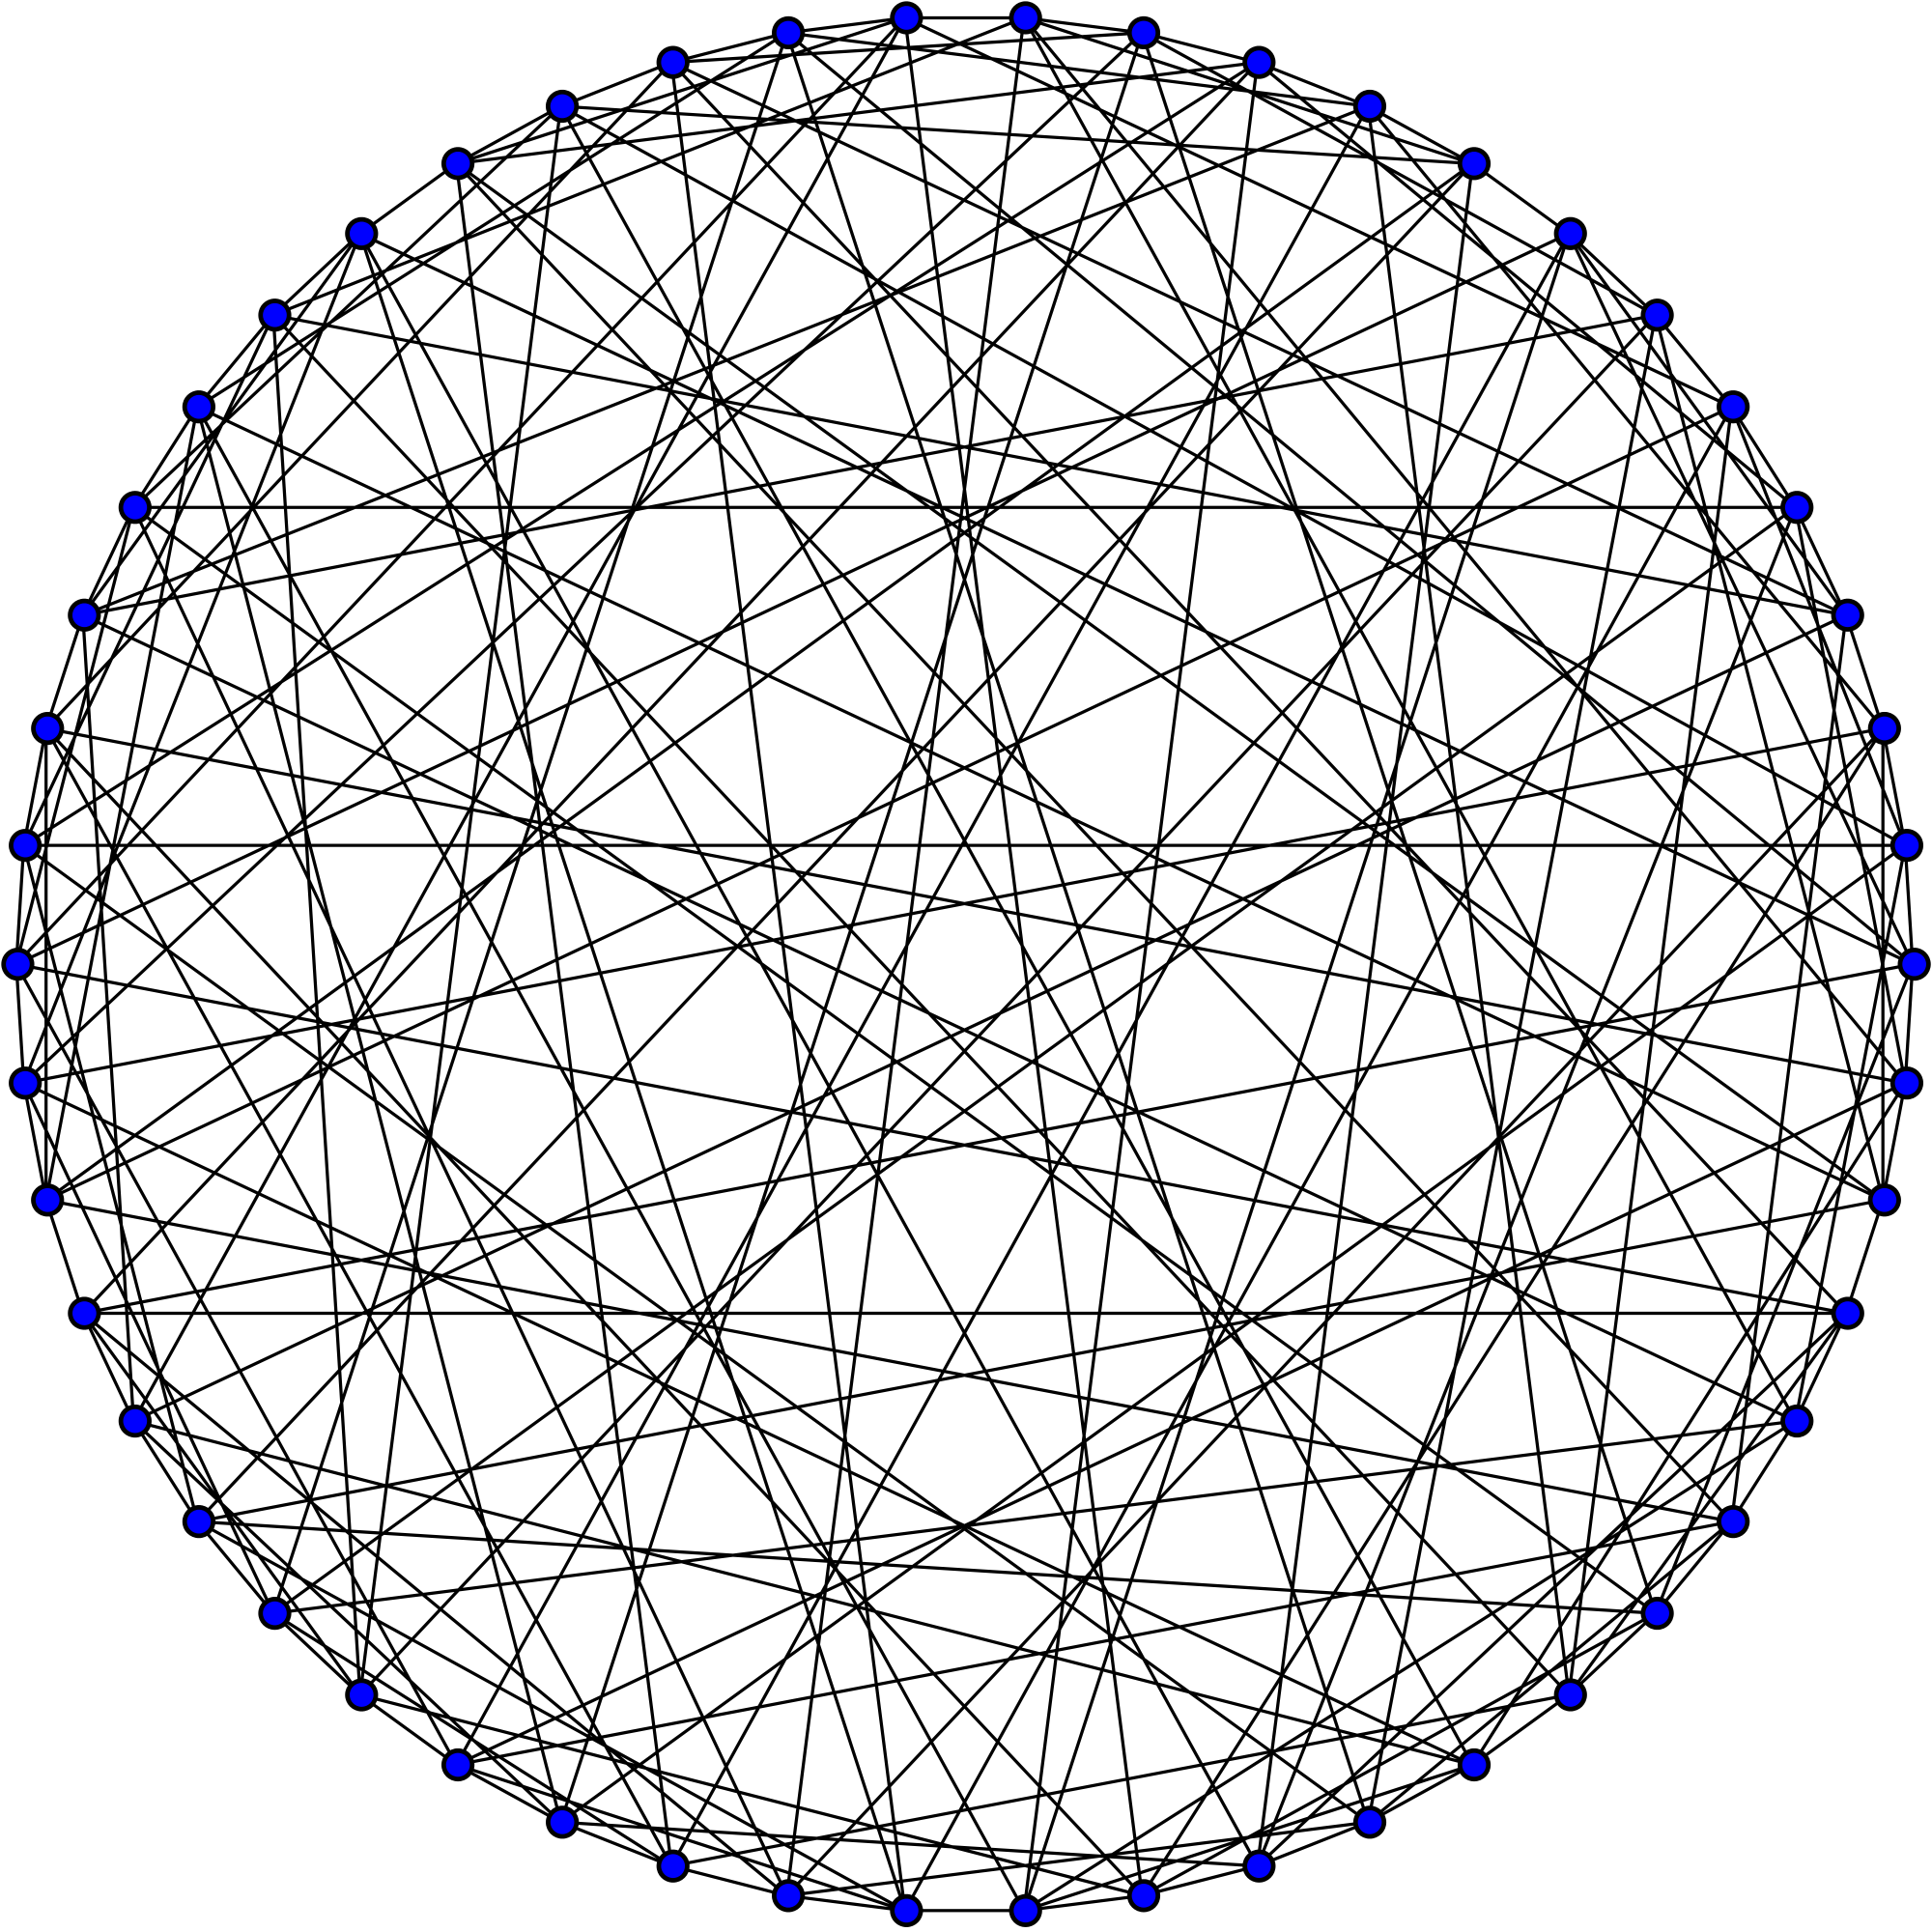
\includegraphics[scale=0.15]{hoffman_singleton}
    \caption*{The unique \hyperlink{def:regular}{7-regular} \hyperlink{def:moore}{Moore} graph}
    \label{fig:hsgraph}
\end{figure}
\clearpage
\section{Introduction}

\subsection{Preliminary}
This course has no prerequisites, being the first course in the tripos in this field.  However, introductory facts about, say, eigenvalues and limits will be used.
As usual, books are not required, but the most relevant is Modern Graph Theory, B. Bollob\'as.

This course consists of six chapters: corresponding to paragraphs 2 to 7 in the schedules but in a different order. Paragraph 1 is introductory, and hence is split between chapters.

\subsection{Informal definitions}
A \emph{graph} consists of `vertices' with some pairs of vertices joined by `edges'.
\begin{center}
    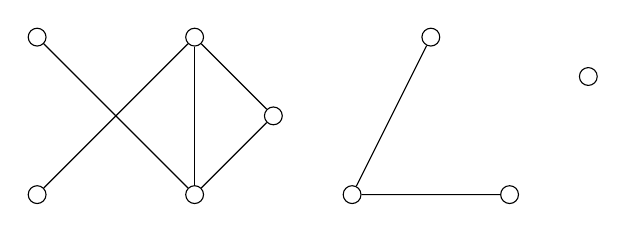
\begin{tikzpicture}
        \node [node] (1) at (0,2) {};
        \node [node] (2) at (2,2) {};
        \node [node] (3) at (0,0) {};
        \node [node] (4) at (2,0) {};
        \node [node] (5) at (3,1) {};

        \node [node] (6) at (5,2) {};
        \node [node] (7) at (4,0) {};
        \node [node] (8) at (6,0) {};

        \node [node] (9) at (7,1.5) {};

        \draw (1) -- (4) -- (5) -- (2) -- (3);
        \draw (2) -- (4);

        \draw (6) -- (7) -- (8);
    \end{tikzpicture}
\end{center}
In this course, we make the following assumptions:
\begin{itemize}
    \item The number of vertices is finite.
    \item No `multiple edges': every pair of vertices is connected by at most one edge.
    \item No loops: no vertex can be joined to itself - edges have to go between different vertices.
\end{itemize}

\subsection{Where do such structures arise?}

\begin{eg}
    \leavevmode
    \begin{enumerate}[label=\arabic*.]
        \item Problem: Can we walk across each bridge in this city precisely once, returning to our starting point? (Euler, 1736: \hypertarget{def:konig}Bridges of K\"onigsberg)
            \begin{center}
                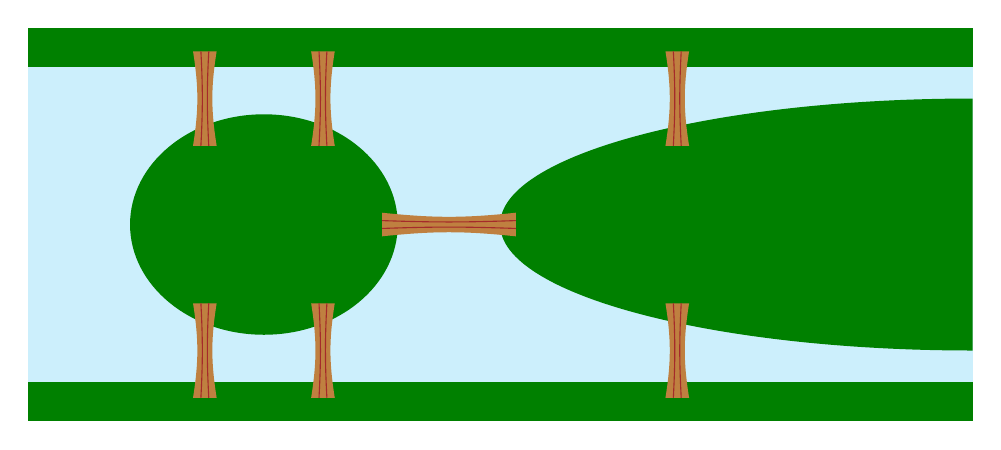
\begin{tikzpicture}
                    \fill [white!80!cyan] (-6,2) rectangle (6,-2);
                    \fill [Green] (-6,2.5) rectangle (6,2);
                    \fill [Green] (-6,-2.5) rectangle (6,-2);
                    \fill [Green] (-3,0) circle [x radius=1.7cm, y radius=1.4cm];
                    \fill [Green] (6,1.6) arc [x radius=6cm, y radius=1.6cm, start angle=90, end angle=270];

                    \fill [brown] (-3.9, 2.2) to [bend left= 9] (-3.9, 1  ) to
                                  (-3.6, 1  ) to [bend left= 9] (-3.6, 2.2) to cycle ;
                    \fill [brown] (-2.1, 2.2) to [bend right=9] (-2.1, 1  ) to
                                  (-2.4, 1  ) to [bend right=9] (-2.4, 2.2) to cycle ;
                    \fill [brown] (-3.9,-2.2) to [bend right=9] (-3.9,-1  ) to
                                  (-3.6,-1  ) to [bend right=9] (-3.6,-2.2) to cycle ;
                    \fill [brown] (-2.1,-2.2) to [bend left= 9] (-2.1,-1  ) to
                                  (-2.4,-1  ) to [bend left= 9] (-2.4,-2.2) to cycle ;
                    \fill [brown] ( 2.1,-2.2) to [bend right=9] ( 2.1,-1  ) to
                                  ( 2.4,-1  ) to [bend right=9] ( 2.4,-2.2) to cycle ;
                    \fill [brown] ( 2.1, 2.2) to [bend left= 9] ( 2.1, 1  ) to
                                  ( 2.4, 1  ) to [bend left= 9] ( 2.4, 2.2) to cycle ;

                    \draw [Brown] (-3.8,-2.2) to [bend right=3] (-3.8,-1);
                    \draw [Brown] (-3.7,-2.2) to [bend left= 3] (-3.7,-1);
                    \draw [Brown] (-2.3,-2.2) to [bend right=3] (-2.3,-1);
                    \draw [Brown] (-2.2,-2.2) to [bend left= 3] (-2.2,-1);
                    \draw [Brown] (-3.8, 2.2) to [bend left= 3] (-3.8, 1);
                    \draw [Brown] (-3.7, 2.2) to [bend right=3] (-3.7, 1);
                    \draw [Brown] (-2.3, 2.2) to [bend left= 3] (-2.3, 1);
                    \draw [Brown] (-2.2, 2.2) to [bend right=3] (-2.2, 1);
                    \draw [Brown] ( 2.3, 2.2) to [bend right=3] ( 2.3, 1);
                    \draw [Brown] ( 2.2, 2.2) to [bend left= 3] ( 2.2, 1);
                    \draw [Brown] ( 2.3,-2.2) to [bend left= 3] ( 2.3,-1);
                    \draw [Brown] ( 2.2,-2.2) to [bend right=3] ( 2.2,-1);

                    \fill [brown] (-1.5, 0.15) to [bend right=6] ( 0.2, 0.15) to
                                  ( 0.2,-0.15) to [bend right=6] (-1.5,-0.15) to cycle;
                    \draw [Brown] (-1.5, 0.05) to [bend right=2] ( 0.2, 0.05);
                    \draw [Brown] (-1.5,-0.05) to [bend left= 2] ( 0.2,-0.05);
                \end{tikzpicture}
            \end{center}

            We turn the problem into a graph problem - in particular, a multigraph to allow multiple edges between vertices.  The vertices of this graph are the four bits of the city, while the edges are the seven bridges.
            In terms of this graph, the problem becomes to walk around the edges of this graph precisely once, and return to the starting vertex.
            \begin{center}
                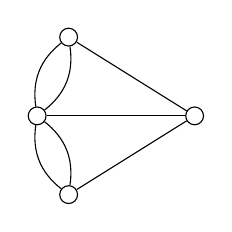
\begin{tikzpicture}[every node/.style=node]
                    \node (A) at (0, 0) {};
                    \node (B) at (0.4, 1) {};
                    \node (C) at (0.4,-1) {};
                    \node (D) at (2,0) {};
                    \draw (A) to [bend left] (B);
                    \draw (A) to [bend right] (B);
                    \draw (A) to [bend left] (C);
                    \draw (A) to [bend right] (C);
                    \draw (A) to (D);
                    \draw (B) to (D);
                    \draw (C) to (D);
                \end{tikzpicture}
            \end{center}

        \item Map colouring problem (1850s)

            How many colours are required to colour a map such that neighbouring countries get different colours?
            \begin{center}
                \begin{tikzpicture}
                    \begin{scope}
                        \draw [clip] circle [x radius=3cm, y radius=2.5cm];
                        \fill [borange] circle [x radius=3cm, y radius=2.5cm];
                        \draw [fill=bred] (0, 5) circle [radius=4.3cm];
                        \draw [fill=bred] (0,-5) circle [radius=4.3cm];
                        \draw [fill=bblue] (-5,0) circle [radius=4cm];
                        \draw [fill=bblue] ( 5,0) circle [radius=4cm];
                    \end{scope}
                    \begin{scope}[yshift=-5cm, every node/.style=node]
                        \node [fill=borange] (A) at (0,0) {};
                        \node [fill=bblue] (B) at (2,0) {};
                        \node [fill=bblue] (C) at (-2,0) {};
                        \node [fill=bred] (D) at (0,1.5) {};
                        \node [fill=bred] (E) at (0,-1.5) {};
                        \draw (B) to (A) to (C) (D) to (A) to (E);
                        \draw (B) to [bend right] (D);
                        \draw (D) to [bend right] (C);
                        \draw (C) to [bend right] (E);
                        \draw (E) to [bend right] (B);
                    \end{scope}
                \end{tikzpicture}
            \end{center}
            Here, the vertices are countries, and the edges are neighbouring pairs.  If we can draw a graph with no crossing edges, how many colours are needed to colour vertices with all edges having two different colours?

        \item Cosets of finite subgroups of finite groups

            Let $G$ be a finite group, $H \leq G$, $|G : H| = n$.  By Lagrange, $\exists a_1, \dots, a_n \in G$ such that the left cosets of $H$ are $a_1 H, \dots a_n H$.
            Similarly, $\exists b_1, \dots, b_n \in G$ such that the right cosets of $H$ are $H a_1, \dots, H a_n$.
            Can we do this simultaneously? In particular, are there $a_1, \dots, a_n \in G$ such that $a_1 H, \dots, a_n H \in G$ are the left cosets, and $H a_1, \dots, H a_n \in G$ are the right cosets?

            In the case where $H \lhd G$ this is easy since we have $a H = H a \; \forall a \in G$.  However it is less obvious if $H \ntriangleleft G$.
            Let $L$ be the set of left cosets, and let $R$ be the set of right cosets. We can create a graph where the vertices are $L \cup R$.
            Join $X \in L$ to $Y \in R$ by an edge if we can find some $a$ such that $X = aH$ and $Y = Ha$, that is, if $X$ and $Y$ have a common element.  Ideally, we would like a graph like this
            (insert bipartite graph here)

            Formally, we ask: In this graph, can we find a set of edges meeting each vertex precisely once?

        \item Fermat equation mod $p$

            Consider the equation $x^n + y^n = z^n$. Does this have solutions mod $p$ for $p$ a prime?  Rule out trivial solutions such as $x = 0, y = z$, in particular we search for solutions in $\mathbb{Z}_p$ where $xyz \ne 0$.
            Let $G = \mathbb{Z} \setminus \{0\}$ under multiplication, and $H = \{g^n : g \in G\}$.  We can check that $H \leq G$, and that $|G : H| \leq n$, by considering the number of $n$th roots an element can have.
            So, $G$ can be partitioned into $g_1 H, g_2 H, \dots, g_mH$ for some $g_1, g_2, \dots, g_m$ and $m \leq n$.  Suppose in some $g_i H$, we have $a, b, c$ with $a + b = c$.  Then $a = g_i x^n, b = g_i y^n, c = g_i z^n$ for some $x, y, z \in G$.  Then
            \begin{align*}
              g_i x^n + g_i y^n &= g_i z^n \\
              x^n + y^n &= z^n
            \end{align*}

            It finally remains to show Schur's Theorem:
    \end{enumerate}
\end{eg}
\begin{thm}[Schur's Theorem]\hypertarget{thm:schur}
    Let $n$ be a positive integer. Then if $p$ is a sufficiently large positive integer, whenever $\{1, 2, \dots, p\}$ is partitioned into $n$ parts, we can solve $a + b = c$ with $a, b, c$ all in some part.
\end{thm}

\clearpage
\section{Ramsey Theory}

\begin{defi}[Graph]\hypertarget{def:graph}
    A \textbf{graph} is an ordered pair $(V, E) = G$ where $V$ is a finite set and $E$ is a set of unordered pairs of distinct elements of $V$.
    We call elements of $V$ \textbf{vertices} of $G$ and elements of $E$ \textbf{edges}.
    We often write $v \in G$ to mean $v \in V$ and sometimes, where clear, $e \in G$ to mean $e \in E$.
    Often denote $\{u, v\} \in E$ by $uv$. Note $uv = vu$.
\end{defi}

\begin{eg}
    Here's an example of a \hyperlink{def:graph}{graph} $G = (\{1, 2, 3, 4, 5, 6, 7\}, \{12, 23, 13, 14, 67\})$, but it's often easier to represent a graph by a drawing: take a point for each \hyperlink{def:graph}{vertex}, join two vertices if they are in an \hyperlink{def:graph}{edge}.
    \begin{center}
        \begin{tikzpicture}[every node/.style = node]
            \node [label=left:$1$]  (1) at ( -1,  0)  {};
            \node [label=above:$2$] (2) at (  0,  1)  {};
            \node [label=below:$3$] (3) at (  0, -1)  {};
            \node [label=right:$4$] (4) at (  1,  0)  {};

            \node [label=above:$5$] (5) at (2.5,  0)  {};
            \node [label=above:$6$] (6) at (  4,  0)  {};
            \node [label=above:$7$] (7) at (5.5,  0)  {};

            \draw (4) -- (1) -- (2) -- (3) -- (1);
            \draw (6) -- (7);
        \end{tikzpicture}
    \end{center}
\end{eg}

\begin{defi}[Isomorphism]\hypertarget{def:gIso}
    Let $G = (V, E)$ and $G' = (V', E')$ be \hyperlink{def:graph}{graphs}.
    An \textbf{isomorphism} from $G$ to $G'$ is a bijection $\phi: V \to V'$ such that for all $u, v \in V$, we have $\phi(u) \phi(v) \in E'$ if and only if $u v \in E$.
    If such an isomorphism exists, we say $G$ is \textbf{isomorphic} to $G'$.
\end{defi}

\begin{defi}[Subgraph]\hypertarget{def:subgraph}
    Suppose also $H = (W, F)$ is a \hyperlink{def:graph}{graph}.
    We say $H$ is a \textbf{subgraph} of $G$ and write $H \subset G$ if $W \subset V$ and $F \subset E$.
    Often, we say `$H$ is a subgraph of $G$' to mean `$H$ is \hyperlink{def:gIso}{isomorphic} to a subgraph of $G$'.
\end{defi}

\begin{defi}[Complete graph of order $n$]\hypertarget{def:Kn}
    The \textbf{complete graph of order $n$}, $K_n$ has $n$ vertices with every pair forming an edge.
\end{defi}

\begin{center}
    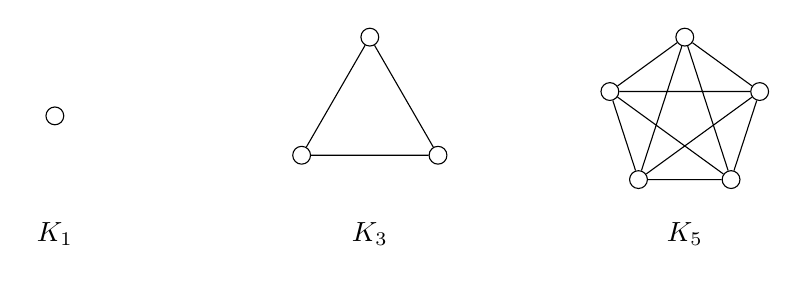
\begin{tikzpicture}
        \begin{scope}
            \node [node] (A) at (0, 0) {};
            \node at (0, -1.5) {$K_1$};
        \end{scope}

        \begin{scope}[xshift=4cm]
            \node [node] (A) at (  90:1)  {};
            \node [node] (B) at (-150:1)  {};
            \node [node] (C) at ( -30:1)  {};

            \draw (A) -- (B) -- (C) -- (A);
            \node at (0, -1.5) {$K_3$};
        \end{scope}

        \begin{scope}[xshift=8cm]
            \node [node] (A) at (  90:1)  {};
            \node [node] (B) at ( 162:1)  {};
            \node [node] (C) at (-126:1)  {};
            \node [node] (D) at ( -54:1)  {};
            \node [node] (E) at (  18:1)  {};

            \draw (A) -- (B) -- (C) -- (D) -- (E) -- (A);
            \draw (A) -- (C) -- (E) -- (B) -- (D) -- (A);
            \node at (0, -1.5) {$K_5$};
        \end{scope}
    \end{tikzpicture}
\end{center}

Looking at the diagram, we see $K_3$ looks like a triangle, and we will often just refer to $K_3$ as a \textbf{triangle}\label{def:triangle}.  In addition, note that if $m \leq n$, then $K_m \subset K_n$.

Recall \hyperlink{thm:schur}{Schur's Theorem}:
\begin{thm}[Schur's Theorem reformulated\label{thm:schur2}]
    Let $k$ be a positive integer. Then there is a positive integer $n$ such that if the set $[n] = \{1, 2, \dots, n\}$ is coloured with $k$ colours, we can find $a, b, c$ with $a + b = c$ and $a,b,c$ the same colour.
\end{thm}

Can we prove this directly? First try $k=1$, where $n=2$ immediately works because $1+1=2$.

For $k=2$, use colours \red{red} and \green{green}, wlog we can take \red{$1$ red}.
As $\red{1}+\red{1}=2$, we must have a \green{green $2$}.
Similarly, \red{$4$} must be \red{red} otherwise $\green{2}+\green{2}=\green{4}$.
Next, we have $\red{1} + 3 = \red{4}$, so \green{$3$} must be \green{green}.
Finally, notice that $\red{1} + \red{4} = \green{2} + \green{3}$ so $n = 5$ suffices.

This case analysis worked for $k=2$, but is likely to get a lot more fiddly for larger $k$.
Even for $k=3$ this case analysis turns out to be a lot harder, so can we come up with a `better' proof for the $k=2$ case, that is `more likely to generalise'?

\begin{proof}($k=2$ of Schur's Theorem, improved)
    Suppose $[5] = \{1, 2, 3, 4, 5\}$ are coloured \red{red} and \green{green}.
    Then some three of these are the same colour, and without loss of generality $\red{i} < \red{j} < \red{k}$ are \red{red}.
    If $j-i$ is \red{red} we are done, since $\red{i} + \red{(j-i)} = \red{j}$.
    Similarly if $k-i$ or $k-j$ is \red{red}, we are done.
    If not, all of $j-i$, $k-i$, $k-j$ are \green{green}, but then $\green{k-i} = \green{(j-i)} + \green{(k-j)}$, and we are done.
\end{proof}

Let's try a similar approach for $k=3$, and I claim $n=16$ works.

\begin{proof}(Schur's theorem, $k=3$)
    Suppose $[16]$ are coloured \red{red}, \green{green} and \blue{blue}.
    By the pigeonhole principle, some six numbers are the same colour, without loss of generality $\red{x_1} < \red{x_2} < \dots < \red{x_6}$ are \red{red}.
    If $x_j - x_i$ is \red{red} for any $i<j$ then we are done: $\red{x_i} + \red{(x_j - x_i)} = \red{x_j}$.
    So assume all $x_j - x_i$ are \blue{blue} or \green{green}.
    Consider the five numbers $x_2 - x_1$, $x_3 - x_1$, $x_4 - x_1$, $x_5 - x_1$, $x_6 - x_1$.
    By the pigeonhole principle, some three of these are the same colour: say $\green{x_i - x_1}$, $\green{x_j - x_1}$, $\green{x_k - x_1}$ are green, for $i < j < k$.

    If $x_j - x_i$ is \green{green}, we are done: $\green{(x_i - x_1)} + \green{(x_j - x_i)} = \green{x_j - x_1}$, similarly if $x_k - x_i$ or $x_k - x_j$ is \green{green}.
    Otherwise, all of $\blue{x_j - x_i}$, $\blue{x_k - x_i}$, $\blue{x_k - x_j}$ are \blue{blue}, and we have $\blue{(x_j - x_i)} + \blue{(x_k - x_j)} = \blue{x_k - x_i}$, so we are done.
\end{proof}

This last paragraph looks very similar to the proof of the $k=2$ case, so can we use induction? It's unclear, because it wasn't exactly the previous case.  But notice how we always seem to be interested in differences of two numbers, yet we never seem to use facts like $7-3 = 9-5$.
So, consider a graph where the vertices are numbers, and the edges refer to the difference between two vertices, and we colour edges.

Suppose the edges of a \hyperlink{def:Kn}{complete graph} $K_6$ are coloured \red{red} and \green{green}. Then we can find a monochromatic \hyperref[def:triangle]{triangle}.
\begin{proof}
    Pick $v \in K_6$. $v$ is in five edges, so some three are the same colour, without loss of generality call them $vx, vy, vz$ and say they are \red{red}.
    If any of $xy, xz, yz$ is \red{red}, we have a \red{red triangle} with $v$.
    If not, $xyz$ is a \green{green triangle}.
    \begin{center}
        \begin{tikzpicture}[scale=1.5, every node/.style=node]
            \begin{scope}
                \node[label=left:$v$]   (v) at ( -0.5, 0) {};
                \node[label=above:$x$]  (x) at (60: 1)    {};
                \node[label=right:$y$]  (y) at ( 1, 0)    {};
                \node[label=below:$z$]   (z) at (-60:1)   {};

                \draw[bgreen, very thick] (x) -- (y) -- (z) -- (x);
                \begin{scope}[bred]
                    \draw (v) -- (x);
                    \draw (v) -- (y);
                    \draw (v) -- (z);
                \end{scope}
            \end{scope}
            \begin{scope}[xshift=-3cm]
                \node[label=left:$v$]   (v) at ( -0.5, 0) {};
                \node[label=above:$x$]  (x) at (60: 1)    {};
                \node[label=right:$y$]  (y) at ( 1, 0)    {};
                \node[label=below:$z$]   (z) at (-60:1)   {};

                \draw[bgreen] (y) -- (z) -- (x);
                \begin{scope}[bred]
                    \draw (v) -- (z);
                    \draw[very thick] (x) -- (y) -- (v) -- (x);
                \end{scope}
            \end{scope}
        \end{tikzpicture}
    \end{center}
\end{proof}

\begin{remark}
    Schur for $k=2$ now follows: Suppose $[5]$ are coloured \red{red}/\green{green}. Take a $K_6$ with vertices $\{0, 1, \dots, 5\}$. Colour edge $ij$, $(i<j)$ with the colour of $j-i$.
    By the above proof, we have a monochromatic \hyperlink{def:triangle}{triangle} $abc$ ($a<b<c$). Then $(c-b) + (b-a) = c-a$, and $c-b, b-a, c-a$ are all the same colour.
    We cannot necessarily find a monochromatic triangle in $K_5$, so 6 vertices are necessary.

    \begin{center}
        \begin{tikzpicture}[scale=2, every node/.style=node]
            \node (A) at (  90:1)  {};
            \node (B) at ( 162:1)  {};
            \node (C) at (-126:1)  {};
            \node (D) at ( -54:1)  {};
            \node (E) at (  18:1)  {};

            \draw[bred] (A) -- (B) -- (C) -- (D) -- (E) -- (A);
            \draw[bgreen] (A) -- (C) -- (E) -- (B) -- (D) -- (A);
        \end{tikzpicture}
    \end{center}

    In this graph form, the statement for more colours is now amenable to an induction proof.
\end{remark}

\begin{nprop}\label{prop:1}
    Let $k$ be a positive integer.
    Then there is a positive integer $n$ such that whenever the edges of $\hyperlink{def:Kn}{K_n}$ are coloured with $k$ colours we can find a monochromatic \hyperlink{def:triangle}{triangle}.
\end{nprop}

\pgfmathsetseed{1}

\begin{proof}
    Induction on $k$. For $k=1$, $n=3$ works, so consider $k>1$.

    By the induction hypothesis, there exists $m$ such that if $\hyperlink{def:Kn}{K_m}$ is $(k-1)$-coloured, then there is a monochromatic \hyperlink{def:triangle}{triangle}.  Let $n = k(m-1) + 2$.

    Now $k$-colour the edges of $K_n$.  Pick vertex $v$.
    The number of edges containing $v$ is $n-1 = k(m-1)+1$.  So some $m$ of them are the same colour, without loss of generality \red{red}.
    Let $H$ be a $K_m$ joined to $v$ by \red{red edges}. If $H$ contains a \red{red edge}, it makes a \red{red triangle} with $v$.
    If not, $H$ is a $(k-1)$-coloured $K_m$ so by definition of $m$, it contains a monochromatic triangle.
    \begin{center}
        \begin{tikzpicture}[scale=0.5]
            \node [node, label=left:$v$] (v) at (0, 0) {};

            \foreach \theta in {25, 15, ..., -25}
                \draw[bred] (v) -- (\theta+rand*3:6+rand*0.4);

            \begin{scope}[xshift=6.5cm, scale=3]
                \draw plot [smooth cycle, tension=0.8] coordinates {(-180:1) (-120:1.2) (-60:0.8) (0:0.9) (60:1.1) (120:1.3)};
                \node at (0.4, 0.6) {$H$};
            \end{scope}
        \end{tikzpicture}
    \end{center}
\end{proof}

\begin{remark}
    \leavevmode
    \begin{enumerate}
        \item Can think in terms of the following picture. Eventually, we will run out of colours and get a monochromatic \hyperlink{def:triangle}{triangle}.
            \begin{center}
                \begin{tikzpicture}[scale=0.6]
                    \node [node] (a) at ( -7,  0) {};
                    \node [node] (b) at ( -4,  1) {};
                    \node [node] (c) at ( -1, -1) {};
                    \node [node] (d) at (1.7,  0) {};

                    \foreach \theta in {38, 36, ..., -36}{
                        \pgfmathsetmacro\rand{rand}
                        \draw [bred]    (a) -- ++(\theta    +\rand*1.4   :  3+\rand*0.5);
                    }
                    \foreach \theta in {30, 28, ..., -28}{
                        \pgfmathsetmacro\rand{rand}
                        \draw [bgreen]  (b) -- ++(\theta*1.1+\rand*1.3-15:  3+\rand*0.5);
                    }
                    \foreach \theta in {24, 22, ..., -22}{
                        \pgfmathsetmacro\rand{rand}
                        \draw [borange] (c) -- ++(\theta*1.4+\rand*1.2+20:2.5+\rand*0.5);
                    }
                    \foreach \theta in {14, 12, ..., -12}{
                        \pgfmathsetmacro\rand{rand}
                        \draw [bblue]   (d) -- ++(\theta*1.6+\rand*1.2+10:2.3+\rand*0.5);
                    }
                    \draw [bred]    (a) -- (b);
                    \draw [bgreen]  (b) -- (c);
                    \draw [borange] (c) -- (d);

                    \draw plot [smooth cycle, tension=0.8, xshift=2.0cm, xscale=2.5, scale=3.0] coordinates {(-180:1.0) (-120:1.2) (-60:0.8) (0:0.9) (60:1.1) (120:1.3)};
                    \draw plot [smooth cycle, tension=0.8, xshift=2.8cm, xscale=2.0, scale=2.6] coordinates {(-180:1.0) (-120:1.2) (-60:0.7) (0:0.9) (60:0.9) (120:1.3)};
                    \draw plot [smooth cycle, tension=0.8, xshift=2.9cm, xscale=1.7, scale=1.8] coordinates {(-180:1.0) (-120:1.3) (-60:0.8) (0:0.9) (60:1.1) (120:1.2)};
                    \draw plot [smooth cycle, tension=0.8, xshift=3.9cm, xscale=1.2, scale=1.0] coordinates {(-180:0.9) (-120:0.9) (-60:0.8) (0:1.1) (60:1.4) (120:1.4)};
                \end{tikzpicture}
            \end{center}

        \item How big do we need to take $n$ to be?  Let $f(k)$ be the smallest $n$ that works with $k$ colours. Clearly $f(1) = 3$. Our proof says for $k>1$, $f(k) \leq k \left(f(k-1)-1\right) + 2 \leq k f(k-1)$.  So by induction, $f(k) \leq 3 k!$.
        \item \nameref{thm:schur2} follows immediately in the same way as for the $k=2$ case.
    \end{enumerate}
\end{remark}

Can we find larger monochromatic subgraphs, for instance a monochromatic \hyperlink{def:Kn}{$K_4$}?
Think about two colours at first for simplicity.  Yes, but we need an intermediate step first.

\begin{eg}
    \leavevmode
    \begin{enumerate}
        \item Let $\hyperlink{def:Kn}{K_{10}}$ have edges coloured \red{red}/\green{green}.
            Then there is a \red{red triangle} or a \green{green $K_4$}.
            \begin{proof}
                Take a vertex $v$. It's in $9$ edges so either $v$ is in \red{$4$ red} edges, or in \green{$6$ green} edges.
                \begin{itemize}
                    \item $v$ is in \red{4 red} edges
                        \begin{center}
                            \begin{tikzpicture}
                                \foreach \ver in {0,1} {
                                    \begin{scope}[xshift=\ver*6 cm]
                                        \node [node,label=left:$v$]  (v\ver) at (-1, 0) {};
                                        \node [node,label=above:$w$] (w\ver) at ( 90:1) {};
                                        \node [node,label=right:$x$] (x\ver) at ( 30:1) {};
                                        \node [node,label=right:$y$] (y\ver) at (-30:1) {};
                                        \node [node,label=below:$z$] (z\ver) at (-90:1) {};

                                        \begin{scope}[bred]
                                            \draw (x\ver) -- (v\ver) -- (w\ver);
                                            \draw (z\ver) -- (v\ver) -- (y\ver);
                                        \end{scope}

                                        \draw[bgreen] (w\ver) -- (x\ver) -- (y\ver) -- (z\ver) -- (w\ver) -- (y\ver);
                                    \end{scope}
                                }

                                \draw [very thick, bred]   (x0) -- (z0) -- (v0) -- (x0);

                                \draw [very thick, bgreen] (w1) -- (x1) -- (y1) -- (z1) -- (w1) -- (y1);
                                \draw [very thick, bgreen] (x1) -- (z1);
                            \end{tikzpicture}
                        \end{center}

                        If any edge between $w, x, y, z$ is \red{red}, we have a \red{red triangle}.

                        If not, they are all \green{green} and we have a \green{green $K_4$}.

                    \item $v$ is in \green{$6$ green} edges
                        \begin{center}
                            \begin{tikzpicture}[scale=0.6]
                                \node [node, label=left:$v$] (v) at (0, 0) {};

                                \foreach \theta in {25, 15, ..., -25}
                                    \draw [bgreen] (v) -- (\theta+rand*3:5+rand*0.5);

                                \begin{scope}[xshift=5cm, scale=3]
                                    \draw plot [smooth cycle, tension=0.8] coordinates {(-180:1.2) (-120:1) (-60:0.8) (0:0.9) (60:1.1) (120:0.9)};
                                    \node [align=center, rectangle] at (0.4, 0.5) {$H$ \\ $(K_6)$};
                                \end{scope}
                            \end{tikzpicture}
                        \end{center}

                        We know $H$ contains a monochromatic triangle. If it is \red{red}, we are done.  If it is \green{green}, then it makes a \green{green $K_4$} with $v$ as required. \qedhere
                \end{itemize}
            \end{proof}
        \item Let $K_{20}$ be coloured \red{red}/\green{green}. Then $\exists$ a monochromatic $K_4$.
            \begin{proof}
                Pick a vertex $v$. It's in $19$ edges, so some $10$ of them are the same colour, without loss of generality \red{red}.

                Let $H$ be a $K_{10}$ joined to $v$ by \red{red} edges.

                Either $H$ has a \red{red triangle}, making a \red{red $K_4$} with $v$, or $H$ contains a \green{green $K_4$}.
            \end{proof}
    \end{enumerate}
\end{eg}

\begin{defi}[\hypertarget{def:ramseyNum}{Ramsey number}]
    Let $s, t \geq 2$. The Ramsey number $R(s, t)$ is the least $n$ such that whenever \hyperlink{def:Kn}{$K_n$} has edges coloured \red{red}/\green{green} there must be a \red{red $K_s$} or a \green{green $K_t$} (if such an $n$ exists).
    We also write $R(s) = R(s, s)$.
\end{defi}

We have seen $\hyperlink{def:ramseyNum}{R(3) = 6}$; $R(3, 4) \leq 10$; $R(4) \leq 20$.

\begin{nthm}[Ramsey's Theorem]\label{thm:ramsey}
    \hyperlink{def:ramseyNum}{$R(s, t)$} exists for all $s, t \geq 2$.
    Moreover, if $s, t > 2$ then $R(s, t) \leq R(s-1, t) + R(s, t-1)$.
\end{nthm}

\begin{proof}
    Induction on $s+t$.

    For $s=2$, we have $\hyperlink{def:ramseyNum}{R(2, t)} = t$: If all edges of a $K_t$ are \green{green}, then we have a \green{green $K_t$}, otherwise there is a \red{red edge}, which is exactly a \red{$K_2$}.  Similarly $R(s, 2) = s$.

    In the case $s, t > 2$, let $a = R(s-1, t)$ and $b = R(s, t-1)$ which exist by the induction hypothesis.  Let $n = a+b$. Suppose $K_n$ has edges coloured \red{red}/\green{green}.
    Pick $v \in K_n$, which is in $a+b-1$ edges, so either $v$ is in \red{$a$ red edges}, or it is in \green{$b$ green edges}.
    \begin{itemize}
        \item If $v$ is in \red{$a$ red edges}, let $H$ be the $K_a$ joined to $v$ by \red{red} edges.  Now $a = R(s-1, t)$, so either $H$ has a \red{red $K_{s-1}$}, making a \red{red $K_s$} with $v$, or $H$ has a \green{green $K_t$}, so done.
        \item If $v$ is in \green{$b$ green edges}, and we can make the same argument with colours reversed. \qedhere
    \end{itemize}
\end{proof}

% cor 3
\begin{ncor}\label{cor:3}
    For all $s, t \geq 2$, $\hyperlink{def:ramseyNum}{R(s, t)} \leq 2^{s+t}$, so $R(s) \leq 4^s$.
\end{ncor}

\begin{proof}
    Induction on $s + t$.  Base cases $s=2$, $R(2, t) = t \leq 2^{2+t}$ and similarly for $t=2$, $R(s, 2) = s \leq 2^{s+2}$.
    For $s, t \geq 2$
    \begin{align*}
        R(s, t) &\leq R(s-1, t) + R(s, t-1) \\
                &\leq 2^{s-1+t} + 2^{s+1-t} \\
                &= 2^{s+t}. \qedhere
    \end{align*}
\end{proof}

\begin{remark}
    \leavevmode
    \begin{itemize}
        \item A more careful version of the same proof gives $\hyperlink{def:ramseyNum}{R(s)} = \hyperlink{def:asymp}{\mathcal{O}} \left(\frac{4^s}{\sqrt{s}}\right)$ (Erd\H{o}s-Szekeres 1935)
        \item A harder proof gives an improvement to $R(s) = \mathcal{O}\left(\frac{4^s}{s}\right)$ (Thomason 1988)
        \item An even harder proof gives $R(s) = \mathcal{O}\left(\frac{4^s}{s^k}\right)$ for any $k$ (Conlon 2009)
        \item Is $R(s) = \mathcal{O}\left(3.999999999^s\right)$? Unknown.
    \end{itemize}
\end{remark}

\begin{nthm}[Multicolour Ramsey Theorem]\label{thm:multiRamsey}
    Let $k \geq 1$ and $s \geq 2$.
    Then there exists some $n$ such that whenever the edges of \hyperlink{def:Kn}{$K_n$} are coloured with $k$ colours, we can find a monochromatic $K_s$.
\end{nthm}

\begin{proof}
    Induction on $k$. For the base case $k=1$, we can take $n=s$.

    For $k>1$, by the induction hypothesis we can find $m$ such that if $\hyperlink{def:Kn}{K_m}$ is $(k-1)$-coloured, then there is a monochromatic $K_s$.
    Let $n = \hyperlink{def:ramseyNum}{R(s, m)}$ and colour $K_n$ with $k$ colours, including \red{red} but not \green{green}.
    Re-colour by turning all non-red edges \green{green}.
    By definition of $n$, we have either
    \begin{itemize}
        \item A \red{red $K_s$}, so done
        \item A \green{green $K_m$}. Then in the original colouring, this $K_m$ was $(k-1)$-coloured, so by definition of $m$, it contains a monochromatic $K_s$. \qedhere
    \end{itemize}
\end{proof}

\begin{remark} \leavevmode
    \begin{enumerate}[label=\arabic*.]
        \item We write $R_k(s)$ for the smallest $n$ that works. In particular $R_1(s) = s$ and $R_2(s) = R(s)$.
            Proof of \Cref{thm:multiRamsey} will give $R_k(s) \leq 4^{s^{k-1}}$.
        \item What do we really mean by colouring?
            We have informally talked about `red edges' etc. More formally, we colouring of the edges of $G = (V, E)$ with $k$ colours is a function $c: E \to [k]$. We mostly refer to the colours as `red', `green' and so on.
            We say $H = (W, F)$ is monochromatic if $c |_F$ is constant.
    \end{enumerate}
\end{remark}

With any number of colours, we can find arbitrarily large monochromatic subgraphs. What about infinite ones?

\begin{defi}[Infinite graph]\hypertarget{def:infGraph}
    An \textbf{infinite graph} is an ordered pair $G = (V, E)$ where $V$ is an infinite set and $E$ is a set of unordered pairs of elements of $V$. Note, in our terminology, an infinite graph is not a graph.
\end{defi}

\begin{defi}[(Possibly infinite) graph]\hypertarget{def:dumbDefi}
    A \textbf{(possibly infinite) graph} is a \hyperlink{def:graph}{graph} or an \hyperlink{def:infGraph}{infinite graph}.
\end{defi}

\begin{defi}[Infinite complete graph]\hypertarget{def:kInf}
    $K_\infty$, the \textbf{infinite complete graph}, is the \hyperlink{def:infGraph}{infinite graph} with a countably infinite vertex set and every pair of vertices forming an edge.
\end{defi}

Where it makes sense to do so, we carry terminology over from graphs to \hyperlink{def:infGraph}{infinite graphs}.
Suppose edges of $\hyperlink{def:kInf}{K_\infty}$ are coloured \red{red}/\green{green}. What can we find? By \nameref{thm:ramsey}, we can find a monochromatic $K_s$ for every finite $s = 1, 2, 3, \dotsc$. Note this doesn't immediately give a monochromatic $K_\infty$:
\begin{center}
    \begin{tikzpicture}[every node/.style=node, scale=0.6]
        \begin{scope}
            \path [scope fading=east] (8, -3) rectangle (25.5, 3);
            \foreach \n in {2,...,9} {
                \begin{scope}[xshift=3*\n cm]
                    \foreach \m in {1,...,\n}{
                        \node (\n\m) at (360/\n*\m+90: 1) {};
                    }
                    \foreach \x in {1,...,\n}{
                        \foreach \y in {1,...,\x} {
                            \draw[bred] (\n\x) -- (\n\y);
                        }
                    }
                \end{scope}
            }
            \begin{scope}[on background layer]
                \foreach \a in {3,...,9} {
                    \pgfmathsetmacro\biggest{\a-1}
                    \foreach \b in {2,...,\biggest} {
                        \foreach \c in {1,...,\a} {
                            \foreach \d in {1,...,\b} {
                                \pgfmathsetmacro\adist{cos(360/\a*\c)}
                                \pgfmathsetmacro\bdist{cos(360/\b*\d)}
                                \pgfmathsetmacro\atop{\adist>0.2?1:0}
                                \pgfmathsetmacro\abot{\adist<-0.2?1:0}
                                \pgfmathsetmacro\btop{\bdist>0.2?1:0}
                                \pgfmathsetmacro\bbot{\bdist<-0.2?1:0}
                                \pgfmathsetmacro\top{\atop+\btop==2?1:0}
                                \pgfmathsetmacro\bot{\abot+\bbot==2?1:0}
                                \ifthenelse{\top=1}{\draw [bgreen, opacity=0.1,path fading=east] (\a\c) to [bend right] (\b\d)}
                                {
                                    \ifthenelse{\bot=1}{\draw [bgreen, opacity=0.1,path fading=east] (\a\c) to [bend left] (\b\d)}
                                    {\draw [bgreen, opacity=0.05,path fading=east] (\a\c) to (\b\d)};
                                };
                            }
                        }
                    }
                }
            \end{scope}
        \end{scope}
    \end{tikzpicture}
\end{center}

In the diagram, we see that for any finite $s$ we have a \red{red $K_s$} but no \red{red $K_\infty$}.
(However in this example, there is a \green{green $K_\infty$})

\begin{nthm}[Infinite Ramsey Theorem]\label{thm:infRamsey}
    Let $k \geq 1$. Whenever the edges of \hyperlink{def:kInf}{$K_\infty$} are $k$-coloured, we have a monochromatic $K_\infty$ subgraph.
\end{nthm}

\begin{proof}
    Take $v_1 \in K_\infty$.  The vertex $v_1$ is in infinitely many edges, so infinitely many edges from $v_1$ are the same colour.
    Let $A_1$ be an infinite set of vertices of $K_\infty$ such that for all $u \in A_1$, $v_1 u$ has colour $c_1$.
    Now pick $v_2 \in A_1$. Similarly, we can find an infinite $A_2 \subset A_1$ such that all edges $v_2 u$ for ($u \in A_2$) have colour $c_2$.
    Keep going. We get infinite sequences $v_1, v_2, v_3, \dotsc$ of vertices, $c_1, c_2, c_3, \dotsc$ of colours and $A_1 \supset A_2 \supset A_3 \supset \dots$ such that
    \begin{itemize}
        \item for $i \geq 2$, $v_i \in A_{i-1}$
        \item for $i \geq 1$, for all $u \in A_i$, $v_i u$ is an edge of colour $c_i$.
    \end{itemize}
    In particular, if $i < j$ then $v_i v_j$ has colour $c_i$. Now, infinitely many of the $c_i$ are the same.
    Say $i_1 < i_2 < i_3 < \dots$ such that $c_{i_1} = c_{i_2} = c_{i_3} = \dotsc$.
    Consider $v_{i_1}, v_{i_2}, v_{i_3}, \dotsc$. Any edge between two of these vertices has colour $c_{i_1}$. So we have a monochromatic $K_\infty$.
\end{proof}

\begin{remark}
    This is often called a `two-pass proof'. On the first pass, we found a sequence of colours, and on the second pass we found infinitely many colours the same.
\end{remark}

\begin{ncor}
    Any bounded sequence has a convergent subsequence.
\end{ncor}

\begin{proof}
    Any bounded monotone sequence converges, so it is enough to show that any real sequence $(x_n)_{n \geq 1}$ has a monotone subsequence.
    Let $G$ be a $K_\infty$ with vertex set $\set{1, 2, 3, \dotsc}$. Colour $ij$, with $i<j$ blue if $x_i < x_j$ and yellow if not.

    By infinite Ramsey, there is a monochromatic subgraph $H \cong K_\infty$. Let the vertices of $H$ be $n_1 < n_2 < n_3 < \dots$.
    If $H$ is blue, then $(x_{n_j})_{j \geq 1}$ is decreasing, whereas if $H$ is yellow then $(x_{n_j})_{j \geq 1}$ is increasing.
\end{proof}

\subsection{Basic Terminology}

Let $G = (V, E)$ be a \hyperlink{def:graph}{graph}. Sometimes write $V(G) = V$, and $E(G) = E$.
The \textbf{order} of $G$ is \hypertarget{def:order}{$\abs{G} = \abs{V(G)}$}. We denote the number of edges of $G$ by \hypertarget{def:eG}{$e(G) = |E(G)|$}, sometimes called the size of $G$.

Note that the \hyperlink{def:Kn}{complete graph of order $n$} has order $n$.

\begin{defi}[Neighbourhood]\hypertarget{def:neighbour}
    Let $v \in G$. Then \textbf{neighbourhood} of $v$ is the set
    \begin{equation*}
        \Gamma(v) = \set{w \in G | vw \in E(G)}
    \end{equation*}

    If $w \in \Gamma(v)$, then $w$ is a \textbf{neighbour} of $v$, or $w$ is \textbf{adjacent} to $v$, we write $w \sim v$.
\end{defi}

\begin{defi}[Degree]\hypertarget{def:degree}
    The \textbf{degree} of $v$ is $d(v) = \abs{\hyperlink{def:neighbour}{\Gamma(v)}}$, the number of vertices \hyperlink{def:neighbour}{adjacent} to $v$.

    The \textbf{maximum degree} of $G$ is $\Delta(G) = \max_{v \in G} d(v)$

    The \textbf{minimum degree} of $G$ is $\delta(G) = \min_{v \in G} d(v)$

    The \textbf{average degree} of $G$ is $\frac{1}{\abs{G}} \sum_{v \in G} d(v)$
\end{defi}

Clearly $\hyperlink{def:degree}{\delta(G)} \leq \text{\hyperlink{def:degree}{average degree} of } G \leq \hyperlink{def:degree}{\Delta(G)}$.

\begin{defi}[Regular]\hypertarget{def:regular}
    If every \hyperlink{def:graph}{vertex} in $G$ has the same \hyperlink{def:degree}{degree}, we say $G$ is \textbf{regular}.
    If this degree is $r$, say $G$ is \textbf{$r$-regular}.
\end{defi}

\begin{eg}
    How do vertex-degrees relate to $\hyperlink{def:eG}{e(G)}$?  We can count `ends of edges' in two different ways.
    In particular, each edge has two ends, so there are $2 e(G)$ ends.
    A vertex $v$ is in $\hyperlink{def:degree}{d(v)}$ ends, so there are $\sum_{v \in G} d(v)$ ends, and hence  $\sum_{v \in G} d(v)= 2 e(G)$.

    Hence also the \hyperlink{def:degree}{average degree} of $G$ is $\frac{2e(G)}{\abs{G}}$.
\end{eg}

\begin{defi}[Path]\hypertarget{def:path}
    Let $G$ be a \hyperlink{def:graph}{graph}. A \textbf{path} in $G$ is a finite sequence $v_0, v_1, \dotsc, v_l$ of distinct vertices of $G$ with $v_{i-1} \hyperlink{def:neighbour}{\sim} v_i$ for $1 \leq i \leq l$.

    \begin{center}
        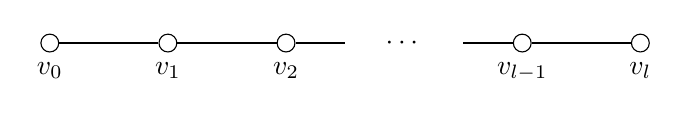
\begin{tikzpicture}[scale=1.5]
            \node [node, label=below:$v_0$]     (0) at (  0,  0)  {};
            \node [node, label=below:$v_1$]     (1) at (  1,  0)  {};
            \node [node, label=below:$v_2$]     (2) at (  2,  0)  {};

            \node [node, label=below:$v_{l-1}$] (3) at (  4,  0)  {};
            \node [node, label=below:$v_l$]     (4) at (  5,  0)  {};

            \node [draw=none] at (3, 0) {$\cdots$};
            \draw (0) -- (1) -- (2) -- (2.5, 0);
            \draw (3.5, 0) -- (3) -- (4);
        \end{tikzpicture}
    \end{center}
    We say this path has length $l$ and goes from $v_0$ to $v_l$.
    \hypertarget{def:to}If $v, w \in G$ we write $v \to w$ to mean there is a path from $v$ to $w$.
\end{defi}

The relation \hyperlink{def:to}{$\to$} is an equivalence relation (Exercise.) % TODO thing about transitivity

\begin{defi}[Components]\hypertarget{def:components}
    The equivalence classes of \hyperlink{def:to}{$\to$} are called the \textbf{components} of $G$.
    If $G$ has only one component, we say $G$ is \textbf{connected}.
    \begin{center}
        \begin{tikzpicture}[every node/.style = node]
            \node (0) at (0, 0)  {};
            \node (1) at (2, 0)  {};
            \node (2) at (1, 1)  {};
            \node (3) at (1,-1)  {};

            \node (4) at (3, 0)  {};
            \node (5) at (4, 1)  {};
            \node (6) at (4,-1)  {};

            \draw (0) -- (1) -- (2) -- (0) -- (3) -- (1);
            \draw (5) -- (4) -- (6);

            \draw [bblue] plot [smooth cycle, tension=0.8] coordinates {(-0.3,0) (1,1.3) (2.3,0) (1,-1.3)};
            \draw [bblue] plot [smooth cycle, tension=0.8] coordinates {(2.7,0) (4.3,1.3) (4.3,-1.3)};
        \end{tikzpicture}
    \end{center}
\end{defi}

\begin{defi}[Cycle]\hypertarget{def:cycle}
    A \textbf{cycle} is a sequence $v_0, v_1, \dotsc, v_l$ of vertices of $G$ with $v_0, \dots, v_{l-1}$ distinct, $v_l = v_0$, $v_{i-1} \hyperlink{def:neighbour}{\sim} v_i$ for $1 \leq i \leq l$ and $l \leq 3$.
    We say that the length of the cycle is $l$.
    \begin{center}
        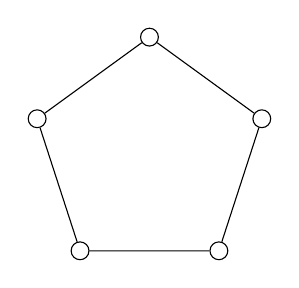
\begin{tikzpicture}[scale=1.5, every node/.style=node]
            \node (A) at (  90:1)  {};
            \node (B) at ( 162:1)  {};
            \node (C) at (-126:1)  {};
            \node (D) at ( -54:1)  {};
            \node (E) at (  18:1)  {};

            \draw (A) -- (B) -- (C) -- (D) -- (E) -- (A);
        \end{tikzpicture}
    \end{center}
\end{defi}

\begin{defi}[Forest]\hypertarget{def:tree}
    A graph with no cycles is called a \textbf{forest}.  A \textbf{tree} is a connected forest.
    Each component of a forest is a tree.
    \begin{center}
        \begin{tikzpicture}[every node/.style = node, scale=1.2]
            \node (0) at (  0,   1) {};
            \node (1) at (  0,   0) {};
            \node (2) at (  0,  -1) {};
            \node (3) at (  1,-1.4) {};
            \node (4) at (  1,-0.3) {};
            \node (5) at ( -1,-0.3) {};

            \node (6) at (  2, 0.5) {};
            \node (7) at (  3,-0.3) {};
            \node (8) at (3.5, 0.4) {};
            \node (9) at (2.4,  -1) {};
            \node (10) at (4, -1) {};

            \node (11) at (4.5, 0.3) {};
            \node (12) at (5, -0.5) {};

            \draw (0) -- (1) -- (5);
            \draw (4) -- (1) -- (2) -- (3);
            \draw (6) -- (7) -- (8);
            \draw (7) -- (9);
            \draw (11) -- (12);
        \end{tikzpicture}
    \end{center}
\end{defi}
\begin{defi}[Disjoint union]\hypertarget{def:disUnion}
    Suppose $G$, $H$ are graphs with $V(G) \cap V(H) = \emptyset$. The \textbf{disjoint union} of $G, H$ is the graph $G \cup H$ with $V(G \cup H) = V(G) \cup V(H)$ and $E(G \cup H) = E(G) \cup E(H)$.

    We often write $G \cup H$ even if $V(G) \cap V(H) \neq \emptyset$, this means take graphs $G', H'$ with $G' \hyperlink{def:gIso}{\cong} G$, $H' \cong H$, $V(G') \cap V(H') = \emptyset$ then take $G' \cup H'$.
\end{defi}

\begin{eg}
    \leavevmode
    \begin{enumerate}
        \item $K_3 \cup K_5$
            \begin{center}
                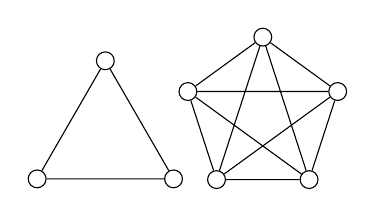
\begin{tikzpicture}
                    \begin{scope}
                        \node [node] (A) at (  90:1)  {};
                        \node [node] (B) at (-150:1)  {};
                        \node [node] (C) at ( -30:1)  {};

                        \draw (A) -- (B) -- (C) -- (A);
                    \end{scope}

                    \begin{scope}[xshift=2cm,yshift=0.3cm]
                        \node [node] (A) at (  90:1)  {};
                        \node [node] (B) at ( 162:1)  {};
                        \node [node] (C) at (-126:1)  {};
                        \node [node] (D) at ( -54:1)  {};
                        \node [node] (E) at (  18:1)  {};

                        \draw (A) -- (B) -- (C) -- (D) -- (E) -- (A);
                        \draw (A) -- (C) -- (E) -- (B) -- (D) -- (A);
                    \end{scope}
                \end{tikzpicture}
            \end{center}
        \item Any graph is the disjoint union of its components $(G_1 \cup \dots \cup G_k)$.
            For instance, a forest is a \hyperlink{def:disUnion}{disjoint union} of trees.
    \end{enumerate}
\end{eg}

\begin{defi}[Induced subgraph]\hypertarget{def:indSubgraph}
    Let $G = (V, E)$ be a graph, and let $W \subset V$. The \textbf{induced subgraph} on $W$ is the graph $G[W]$ with $V(G[W]) = W$ and, for $x,y \in W$, $xy \in E(G[W]) \iff xy \in G$.
\end{defi}

\begin{defi}[Complement]\hypertarget{def:complement}
    Let $G = (V, E)$ be a graph. The \textbf{complement} of $G$ is the graph $\overline{G}$ with $V(\overline{G}) = V$, and for distinct $x, y \in V$, $xy \in E(\overline{G}) \iff xy \notin E$.
\end{defi}

\begin{eg}
    \leavevmode
    \begin{itemize}
        \item Suppose edges of $K_n$ are coloured \red{red}/\green{green}. We can think about the `red subgraph' with $n$ vertices and red edges only.
            The \hyperlink{def:complement}{complement} is the green subgraph.
        \item \hyperlink{def:gIso}{Isomorphic} to its \hyperlink{def:complement}{complement}:
        \begin{center}
            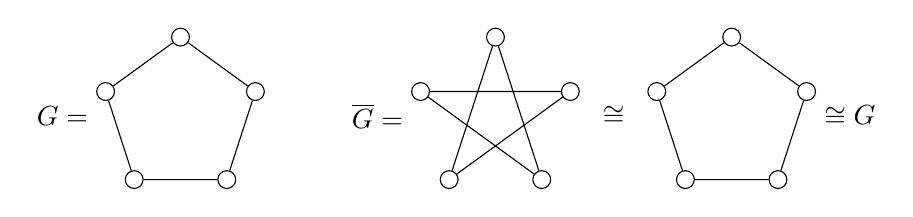
\begin{tikzpicture}
                \node at (-1.5,0) {$G=$};
                \begin{scope}[every node/.style=node]
                    \node (A) at (  90:1)  {};
                    \node (B) at ( 162:1)  {};
                    \node (C) at (-126:1)  {};
                    \node (D) at ( -54:1)  {};
                    \node (E) at (  18:1)  {};
                    \draw (A) -- (B) -- (C) -- (D) -- (E) -- (A);
                \end{scope}
                \node at (2.5,0) {$\overline{G}=$};
                \begin{scope}[every node/.style=node, xshift=4cm]
                    \node (A) at (  90:1)  {};
                    \node (B) at ( 162:1)  {};
                    \node (C) at (-126:1)  {};
                    \node (D) at ( -54:1)  {};
                    \node (E) at (  18:1)  {};
                    \draw (A) -- (C) -- (E) -- (B) -- (D) -- (A);
                \end{scope}
                \node at (5.5,0) {$\cong$};
                \begin{scope}[every node/.style=node, xshift=7cm]
                    \node (A) at (  90:1)  {};
                    \node (B) at ( 162:1)  {};
                    \node (C) at (-126:1)  {};
                    \node (D) at ( -54:1)  {};
                    \node (E) at (  18:1)  {};
                    \draw (A) -- (B) -- (C) -- (D) -- (E) -- (A);
                \end{scope}
                \node at (8.5,0) {$\cong G$};
            \end{tikzpicture}
        \end{center}

    \end{itemize}
\end{eg}

\begin{notation}\hypertarget{def:asymp}
    Let $f, g: \N \to (0, \infty)$.
    We say
    \begin{itemize}[label={--}]
        \item $f = \mathcal{O}(g)$ if $f < A g$ for some constant $A$.
        \item $f = \Omega(g)$ if $g = \mathcal{O}(f)$
        \item $f = \Theta(g)$ if $f = \mathcal{O}(g)$ and $f = \Omega(g)$.

        \item $f = o(g)$ means $f/g \to 0$ (as $n \to \infty$)
        \item $f = \omega(g)$ means $f/g \to \infty$
        \item $f \sim g$ means $f/g \to 1$.
    \end{itemize}
\end{notation}

\clearpage
\section{Extremal Graph Theory}

\textbf{Problem} (from section 1): How large must $n$ be so that if edges of \hyperlink{def:Kn}{$K_n$} are coloured \red{red}/\green{green} then always get a monochromatic $K_s$?

Let $G$ be a `\red{red} subgraph' of $K_n$, consisting of all vertices, and only the \red{red} edges.
$K_n$ has a \red{red} $K_s \iff K_s \subset G$, and $K_n$ has a \green{green} $K_s \iff G$ has an \hyperlink{def:indSubgraph}{induced} $\hyperlink{def:complement}{\overline{K_s}}$ subgraph.

\textbf{Rephrased}:
How large must $n$ be to force every graph of order $n$ to have $K_s$ or $\overline{K_s}$ as an induced subgraph?

This is a typical example of an \textbf{extremal problem}: How large must some parameter of $G$ be to force $G$ to have a certain property?
Alternatively, how big can the parameter be with $G$ not having the property?

\subsection{Forbidden Subgraph Problem}
Fix a \hyperlink{def:graph}{graph} $H$ with at least one edge. Let $n \geq \abs{H}$. Clearly $H \subset K_n$ but $H \not\subset \overline{K_n}$.

How many edges must a graph $G$ of order $n$ have to force $H \subset G$? Alternatively, if $\abs{G} = n$ and $H \subset G$, how large can $\hyperlink{def:eG}{e(G)}$ be?

\begin{defi}[Extremal number]\hypertarget{def:exn}
    Define
    \begin{equation*}
        \ext(n; H) = \max\set{\hyperlink{def:eG}{e(G)} | \abs{G} = n, H \not\subset G}
    \end{equation*}
\end{defi}

\paragraph{Problem} Can we determine $\hyperlink{def:exn}{\ext}(n; H)$?

\subsubsection{Triangles}
Let $H = K_3$. The goal is to find $G$ with $\abs{G} = n$, $\hyperlink{def:eG}{e(G)}$ large and $\triangle \not\subset G$.
The idea is to partition $V(G) = X \cup Y$ with all edges going from $X$ to $Y$.

\begin{defi}[Bipartite graph]\hypertarget{def:bipartite}
    A graph $G$ is \textbf{bipartite} (with bipartition $(X, Y)$) if $V(G)$ can be partitioned as $X \cup Y$ in such a way that if $e \in E(G)$ then $e = xy$ for some $x \in X$, $y \in Y$.
\end{defi}

Bipartite graphs have no $\triangle$s (and indeed no cycles of odd length). In fact the converse is also true:
\begin{nthm}\label{thm:7}
    A graph is bipartite iff it contains no odd cycles.
\end{nthm}

\begin{proof}
    May return to this later, an exercise for now.
\end{proof}

Which \hyperlink{def:bipartite}{bipartite graph} is best?
Clearly it is a good idea to include all possible edges from $X$ to $Y$.

\begin{defi}[Complete bipartite graph]\hypertarget{def:knn}
    Let $s, t \geq 1$. The \textbf{complete bipartite graph} $K_{s, t}$ has \hyperlink{def:bipartite}{bipartition} (X, Y) with $\abs{X} = s$, $\abs{Y} = t$ and $xy \in E(K_{s, t})$ $\forall x \in X, y \in Y$.
\end{defi}

We have $\abs{K_{s, t}} = s + t$ and $e(K_{s, t}) = st$, and aim to maximise $st$ subject to $s + t = n$, that is, maximise $s(n-s)$.
So, the best \hyperlink{def:bipartite}{bipartite graph} is $\hyperlink{def:knn}{K_{\ceil{\frac{n}{2}}, \floor{\frac{n}{2}}}}$
But what if some non-bipartite graph is better?
In fact, the bipartite graph always wins:

\begin{nthm}[Mantel's Theorem]\label{thm:8}
    Let $n \geq 3$. Suppose $\abs{G} = n$, $e(g) \geq \floor{\frac{n^2}{4}}$ and $\triangle \not\subset G$.
    Then $G \cong K_{\ceil{\frac{n}{2}}, \floor{\frac{n}{2}}}$.
\end{nthm}

\begin{proof}
    Induction on $n$. Start with the $n=3$ case: Consider $K_{2, 1}$, it satisfies $\abs{G} = 3$, $\hyperlink{def:eG}{e(G)} \geq 2$, $\triangle \subset G$, as required.

    $n>3$: Let $\abs{G} = n$, $e(G) \geq \floor{\frac{n^2}{4}}$, $\triangle \not\subset G$.
    First, remove edges from $G$ if necessary to get $H$ with $\abs{H} = n$, $e(H) = \floor{\frac{n^2}{4}}$. Clearly $\triangle \not\subset H$.
    Let $v \in H$ with $d(v) = \hyperlink{def:degree}{\delta(H)}$ and let $K = H - v$ (i.e.\ $H$ with vertex $v$ and all edges including $v$ removed).
    Now, $\abs{K} = n-1$, $\triangle \not\subset K$ and $e(K) = \floor{\frac{n^2}{4}} - \delta(H)$.

    Suppose $n$ is even. Then $\delta(H) \leq \text{average degree of } H = \frac{2 e(H)}{H} = \frac{n^2/2}{n} = \frac{n}{2}$.
    Hence
    \begin{equation*}
    e(K) \geq \frac{n^2}{4} - \frac{n}{2} = \frac{n^2 - 2n}{4} = \frac{n^2 - 2n + 1}{4} - \frac{1}{4} = \frac{(n-1)^2}{4} - \frac{1}{4} = \floor*{\frac{(n-1)^2}{4}}\end{equation*}
    Similarly if $n$ odd, also get $e(K) \geq \floor*{\frac{(n-1)^2}{4}}$.

    Hence by the induction hypothesis, $K \cong K_{\ceil{\frac{n-1}{2}}, \floor{\frac{n-1}{2}}}$.
    Also, $d(v) = e(H) - e(K)$.
    If $n$ even, $d(v) = \frac{n^2}{4} - \frac{n^2 - 2n}{4} = \frac{n}{2}$.
    $H$ is formed by adding a vertex $v$ to $K \cong K_{\frac{n}{2}, \frac{n-2}{2}}$ and joining $v$ to $\frac{n}{2}$ vertices of $K$, without creating a triangle.

    If $K$ has bipartition $(X, Y)$, $v$ cannot be joined both to a vertex in $X$ and a vertex in $Y$. So $v$ must be joined to all vertices in the larger of $X$, $Y$.
    Thus $H \cong K_{\ceil{\frac{n}{2}}, \floor{\frac{n}{2}}}$ and similarly if $n$ is odd.
    We recover $G$ by adding edges to $H$ without making a $\triangle$. But any new edge creates a $\triangle$, so $G \cong H$.
\end{proof}

Hence if $\abs{G} = n$, $\hyperlink{def:eG}{e(G)} > \floor{\frac{n^2}{4}}$ then $\triangle \subset G$. Therefore $\ext(n; \triangle) = \floor{\frac{n^2}{4}}$.

\subsubsection{Complete graphs}
What about if we are trying to avoid a $K_4$? Try a complete tri-partite graph.

\begin{defi}[$r$-partite graph]\hypertarget{def:rpartite}
    A graph $G$ is \textbf{$r$-partite} if we can partition $V(G) = X_1 \cup \dotsb \cup X_r$ in such a way that if $xy \in E(G)$ then $x \in X_i, y \in X_j$ for some $i \neq j$.
    We say $G$ is \textbf{complete $r$-partite} if whenever $x \in X_i$, $y \in X_j$ with $i \neq j$ then $x y \in E(G)$.
\end{defi}

\begin{defi}[Tur\'{a}n graph]\hypertarget{def:turan}
    The \textbf{Tur\'{a}n graph} $T_r(n)$ is the complete $r$-partite graph with $n$ vertices and vertex-classes as equal as possible. Write $t_r(n) = e(T_r(n))$.
\end{defi}

\begin{eg}
    \leavevmode
    \begin{itemize}
        \item $\hyperlink{def:turan}{T_2(n)} = \hyperlink{def:knn}{K_{\floor{\frac{n}{2}}, \ceil{\frac{n}{2}}}}$
        \item The diagram shows $T_3(7)$.
            \begin{center}
                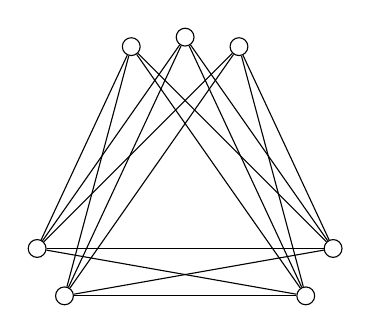
\begin{tikzpicture}[every node/.style=node]
                    \node (a1) at ( 70:2) {};
                    \node (a2) at ( 90:2) {};
                    \node (a3) at (110:2) {};
                    \node (b1) at (-20:2) {};
                    \node (b2) at (-40:2) {};
                    \node (c1) at (200:2) {};
                    \node (c2) at (220:2) {};
                    \foreach \x in {1,2,3}
                        \foreach \y in {1,2}{
                        \draw (a\x) -- (b\y);
                        \draw (a\x) -- (c\y);}
                    \foreach \x in {1,2}{\foreach \y in {1,2} \draw (b\x) -- (c\y);}
                \end{tikzpicture}
            \end{center}
    \end{itemize}
\end{eg}

\begin{remark}[Properties of the Tur\'{a}n graph]\leavevmode
\begin{enumerate}
    \item $\hyperlink{def:Kn}{K_{r+1}} \not\subset \hyperlink{def:turan}{T_r(n)}$. If we add an edge to $T_r(n)$ we create a $K_{r+1}$.
    \item $T_r(n)$ has more edges than any other $r$-partite graph on $n$ vertices. Suppose $G$ is a complete $r$-partite graph with some two vertex classes $X, Y$ with $\abs{Y} > \abs{X}+1$.
        Moving a vertex from $Y$ to $X$ loses $\abs{X}$ edges but gains $\abs{Y}-1 > \abs{X}$ edges.
    \item If $r \mid n$ then all classes of $T_r(n)$ are same.
        If $r \nmid n$ then we have `small' classes, with $k$ vertices, say, and `big' classes with $k+1$ vertices.
    \item If $r \mid n$ then $T_r(n)$ is regular.
        If $r \nmid n$ then if $v$ in the big class, $d(v) = \delta(T_r(n))$ and if $v$ is in the small class $d(v) = \hyperlink{def:degree}{\Delta}(T_r(n)) = \delta(T_r(n)) + 1$
        So in general, vertex degrees in $T_r(n)$ differ by at most 1.
    \item Deleting a vertex of minimal degree from $T_r(n)$ removes a vertex from a big class, thus making $T_r(n-1)$.
        So $\hyperlink{def:turan}{t_r(n-1)} = t_r(n) - \hyperlink{def:degree}{\delta}(T_r(n))$.
    \item Suppose we have $T_r(n-1)$. Add a vertex $v$. How many edges can we add without creating a $K_{r+1}$? We can't join $v$ to a vertex in every class so must miss some class.

        So the best is to join $v$ to all vertices except those in a particular small class $X$.
        Same as adding $v$ to class $X$, so we've made $T_r(n)$. So \# of edges we can add is at most $t_r(n) - t_r(n-1)$ and only way to achieve this makes $T_r(n)$.
\end{enumerate}
\end{remark}

\begin{nthm}[Tur\'{a}n's Theorem]\label{thm:9}
    Let $r \geq 2$ and $\abs{G} = n \geq r+1$. If $\hyperlink{def:eG}{e(G)} \geq \hyperlink{def:turan}{t_r(n)}$ and $\hyperlink{def:Kn}{K_{r+1}} \not\subset G$ then $G \cong T_r(n)$.
\end{nthm}

\begin{proof}
    Induction on $n$.
    Take first $n = r+1$. $T_r(r+1)$ has one class of 2 vertices, rest with 1 vertex each. So $T_r(r+1)$ is $K_{r+1}$ with 1 edge removed. So $G \cong T_r(r+1)$.

    Next consider $n > r+1$. First delete edges from $G$ to form subgraph $H$ with $\abs{H} = n$, $e(H) = t_r(n)$ and $K_{r+1} \not \subset H$. Let $v \in H$ have minimal degree and let $K = H- v$.
    We know $\abs{H} = \abs{T_r(n)}$ and $e(H) = e(T_r(n))$ so $H$ and $T_r(n)$ have same \hyperlink{def:degree}{average degree}. But degrees in $T_r(n)$ are as equal as possible by property 4 earlier.

    So $\hyperlink{def:degree}{\delta(H)} \leq \delta(T_r(n))$. Thus $\abs{K} = n-1$, $K_{r+1} \not\subset K$ and \begin{align*}e(K) = e(H) - \delta (H) \geq e(H) - \delta(T_r(n)) = t_r(n) - \delta(T_r(n)) = t_r(n-1)\end{align*} by 5.
    So by induction hypothesis, $K \cong T_r(n-1)$. And $d(v) = e(H) - e(K) = t_r(n) - t_r(n-1)$.
    To recover $H$, we must add a vertex and $t_r(n) - t_r(n-1)$ edges to $K$ without creating a $K_{r+1}$. So by 6, $H \cong T_r(n)$.
    To recover $G$, add edges to $H$ without creating a $K_{r+1}$. But by property 1 we can't add any edges. So, $G \cong T_r(n)$.
\end{proof}

So if $r \geq 2$, $n \geq r+1$, $\hyperlink{def:exn}{\ext}(n; \hyperlink{def:Kn}{K_{r+1}}) = \hyperlink{def:turan}{t_r(n)}$.
How big is $t_r(n)$ approximately?
Each vertex is joined to a proportion approximately $1 - \frac{1}{r}$ of all vertices, so we have a proportion approx $1 - \frac{1}{r}$ of all possible edges. So $\ext(n; K_{r+1}) \approx (1-\frac{1}{r}) \binom{n}{2}$.
More precisely,

\begin{ncor}\label{cor:10}
    Let $r \geq 2$. As $n \to \infty$, $\hyperlink{def:exn}{\ext(n; K_{r+1})} \hyperlink{def:asymp}{\sim} (1 - \frac{1}{r}) \binom{r}{2}$.
\end{ncor}

\subsubsection{Bipartite graphs}
Can think of \hyperlink{def:cycle}{cycles} and \hyperlink{def:path}{paths} as \hyperlink{def:graph}{graphs} (ignore direction and start point).

\begin{defi}[Cyclic graph]\hypertarget{def:Cn}
    The \textbf{cyclic graph of order $n$}, is the \hyperlink{def:cycle}{cycle} of length $n$, called $C_n$.
    \begin{center}
        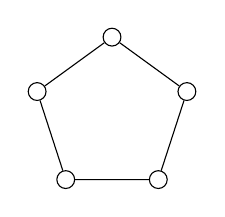
\begin{tikzpicture}[every node/.style=node]
            \node (A) at (  90:1)  {};
            \node (B) at ( 162:1)  {};
            \node (C) at (-126:1)  {};
            \node (D) at ( -54:1)  {};
            \node (E) at (  18:1)  {};
            \draw (A) -- (B) -- (C) -- (D) -- (E) -- (A);
        \end{tikzpicture}
    \end{center}
\end{defi}

\begin{defi}[Path graph]\hypertarget{def:Pn}
    The \textbf{path graph} of order $n$ is the \hyperlink{def:path}{path} of length $n$, called $P_n$.
    \begin{center}
        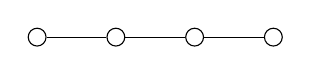
\begin{tikzpicture}[every node/.style=node]
            \node (A) at (0,0) {};
            \node (B) at (1,0) {};
            \node (C) at (2,0) {};
            \node (D) at (3,0) {};
            \draw (A) -- (B) -- (C) -- (D);
        \end{tikzpicture}
    \end{center}
\end{defi}

So $\abs{\hyperlink{def:Cn}{C_n}} = n$, $\abs{\hyperlink{def:Pn}{P_n}} = n+1$, and $e(C_n) = e(P_n) = n$.

\begin{eg}
    What can we say about $\hyperlink{def:exn}{\ext}(n; \hyperlink{def:Cn}{C_4})$? Note $C_4 \cong \hyperlink{def:knn}{K_{2, 2}}$.
    \begin{center}
        \begin{tikzpicture}[every node/.style=node, scale=0.7]
            \begin{scope}
                \node[bred]   (1) at (1,0) {};
                \node[bgreen] (2) at (0,1) {};
                \node[bred]   (3) at (1,2) {};
                \node[bgreen] (4) at (2,1) {};

                \draw (1) -- (2) -- (3);
                \draw (1) -- (4) -- (3);
            \end{scope}
        \end{tikzpicture}
    \end{center}
    $C_4$ is made from two copies of \hyperlink{def:Pn}{$P_2$}. Suppose $G$ is a graph, $\abs{G} = n$, $ \hyperlink{def:eG}{e(G)} = m$, and $C_4 \not\subset G$. How many $P_2$ subgraphs does $G$ have?
    Given $v \in G$, $v$ is the middle vertex of $\binom{d(v)}{2}$ $P_2$s.
    So the total number of $P_2$s is $\sum_{v \in G} \binom{d(v)}{2}$.

    On the other hand, observe that if $\{x, y\} \subset V(G)$ with $x \neq y$ then there is at most one $P_2$ where $x, y$ are end vertices (because $C_4 \not\subset G$). So, the number of $P_2$s is $\leq \binom{n}{2}$.
    \begin{center}
        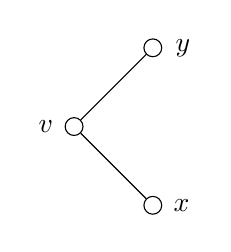
\begin{tikzpicture}[every node/.style=node]
            \node[label=right:$x$] (1) at (1,0) {};
            \node[label=left:$v$] (2) at (0,1) {};
            \node[label=right:$y$] (3) at (1,2) {};
            \draw (1) -- (2) -- (3);
        \end{tikzpicture}
    \end{center}
    Hence \begin{equation*}\sum_{v \in G} \binom{d(v)}{2} \leq \binom{n}{2}\end{equation*}
    Recall Jensen's Inequality: for a convex function $f$,
    \begin{equation*}
        \frac{1}{n} \sum_{i=1}^n f(x_i) \geq f\left(\frac{1}{n} \sum_{i=1}^n x_i\right)
    \end{equation*}
    Apply Jensen to the earlier bound to give
    \begin{equation*}
        \binom{n}{2} \geq \sum_{v \in G} \binom{d(v)}{2} \geq n \binom{\frac{1}{n} \sum_{v \in G} d(v)}{2} = n \binom{2 \frac{m}{n}}{2}
    \end{equation*}
    Hence $n(n-1) \geq n \frac{2m}{n} (\frac{2m}{n} - 1)$, so $n^2 (n-1) \geq 2m (2m-n)$ so $4m^2 - 2mn - n^2 (n-1) \leq 0$.
    This is a quadratic in $m$ with roots
    \begin{align*}
        m &= \frac{2n \pm \sqrt{4 n^2 + 16 n^2(n-1)}}{8} \\
        &= \frac{n}{4}(1 \pm \sqrt{1 + 4\left(n-1\right)}) \\
        &= \frac{n}{4}\left(1 \pm \sqrt{4n - 3}\right)
    \end{align*}
    Hence $m \leq \frac{n}{4}\left(1 + \sqrt{4n-3}\right)$, so $\hyperlink{def:exn}{\ext(n; C_4)} \leq \frac{n}{4} \left(1 + \sqrt{4n-3}\right)$, and so $\ext(n; C_4) = \hyperlink{def:asymp}{\mathcal{O}}\left(n^\frac{3}{2}\right)$.
    A similar approach turns out to give a bound on $\ext(n; K_{t, t})$ in general:
    \begin{center}
        \begin{tikzpicture}[every node/.style=node]
            \begin{scope}
                \node (11) at (1,1) {};
                \node (12) at (1,2) {};
                \node (21) at (2,1) {};
                \node (22) at (2,2) {};

                \draw[bred]   (21) -- (11) -- (22);
                \draw[bgreen] (21) -- (12) -- (22);
            \end{scope}

            \begin{scope}[xshift=3cm]
                \foreach \y in {1,2,3} {
                    \node (1\y) at (1, \y) {};
                    \node (2\y) at (2, \y) {};
                };
                \foreach \y in {1,2,3} {
                    \draw[bgreen] (2\y) -- (11);
                    \draw[bred]   (2\y) -- (12);
                    \draw[bblue]  (2\y) -- (13);
                };

            \end{scope}
        \end{tikzpicture}
    \end{center}
\end{eg}

\begin{defi}[$t$-fan]\hypertarget{def:fan}
    A \textbf{t-fan} in a graph $G$ is an ordered pair $(v, W)$ where $v \in V(G)$, $W \subset V(G)$, $\abs{W} = t$ and $\forall w \in W$, $v \sim w$.
\end{defi}

\begin{eg}
    \hyperlink{def:fan}{$2$-fans} correspond to \hyperlink{def:Pn}{$P_2$} subgraphs.
\end{eg}

\begin{nthm}\label{thm:11}
    Let $t \geq 2$. Then $\hyperlink{def:exn}{\ext}(n; \hyperlink{def:knn}{K_{t,t}}) = \hyperlink{def:asymp}{\mathcal{O}}\left(n^{2 - \frac{1}{t}}\right)$.
\end{nthm}

\begin{proof}
    Let $\abs{G} = n$, $\hyperlink{def:eG}{e(G)} = m = \ext(n; K_{t, t})$ and $K_{t,t} \not\subset G$.
    How many \hyperlink{def:fan}{$t$-fans} are there in $G$?
    Each $v \in G$ is in $\binom{d(v)}{t}$ $t$-fans.
    This total number is $\sum_{v \in G} \binom{d(v)}{t}$.

    Given $W \subset V(G)$ with $\abs{W} = t$, $W$ is in at most $t-1$ $t$-fans (as $K_{t, t} \not\subset G$).
    So the total number of $t$-fans is $\leq \binom{n}{t} (t-1)$.
    Hence
    \begin{align*}
        \binom{n}{t} (t-1) &\geq \sum_{v \in G} \binom{d(v)}{t} \\
                           &\geq n \binom{\frac{1}{n} \sum_{v \in G} d(v)}{t} \qquad \text{by Jensen}\\
                           &= n \binom{\frac{2m}{n}}{t}
    \end{align*}

    So $\frac{n^t}{t!} (t-1) \geq \frac{n}{t!} (\frac{2m}{n} - t)^t$, taking the highest factor from the LHS and lowest factor from the RHS so \begin{equation*}n^t (t-1) \geq n \left(\frac{2m}{n} - t\right)^t.\end{equation*}
    If $n$ is sufficiently large (as we may assume) then $m \geq n t$ and so $\frac{m}{n} \geq t$ and so $\frac{2m}{n} - t \geq \frac{m}{n}$.
    Thus
    \begin{align*}
        n^t (t-1) &\geq n \left(\frac{m}{n}\right)^t \\ m^t &\leq n^{2t-1} (t-1) \\
        m &\leq (t-1)^\frac{1}{t} n^{2-\frac{1}{t}} = \hyperlink{def:asymp}{\mathcal{O}}(n^{2-\frac{1}{t}}). \qedhere
    \end{align*}
\end{proof}

We will see lower bounds later.
Closely related is the \textbf{Problem of Zarankiewicz}.
\hypertarget{def:zara}Let $z(n, t)$ be the largest possible number of edges in a \hyperlink{def:bipartite}{bipartite} graph $G$ with $n$ vertices in each class and $K_{t, t} \not\subset G$.

\begin{nthm}\label{thm:12}
    Let $t \geq 2$. Then $z(n, t)  = \hyperlink{def:asymp}{\mathcal{O}}(n^{2 - \frac{1}{t}})$.
\end{nthm}
\begin{proof}
    Let $G$ be \hyperlink{def:bipartite}{bipartite} with classes $X$, $Y$ with $\abs{X} = \abs{Y} = n$, $\hyperlink{def:eG}{e(G)} = m = z(n, t)$ and $K_{t, t} \not\subset G$.
    Count number of \hyperlink{def:fan}{$t$-fans} with vertex in $X$ and set in $Y$.
    Similar to the proof of \cref{thm:11},
    \begin{equation*}
        \binom{n}{t} (t-1) \geq \sum_{v \in X} \binom{d(v)}{t}
    \end{equation*}
    Now $\sum_{v \in X} d(v) = m$, so a similar calculation to \cref{thm:11} gives $m = \hyperlink{def:asymp}{\mathcal{O}}(n^{2 - \frac{1}{t}})$.
\end{proof}

\subsubsection{General graphs}

What is $\hyperlink{def:exn}{\ext(n; H)}$? This is a hard question, and we could not even find an exact answer for $H = \hyperlink{def:Cn}{C_4}$, so instead consider some asymptotics.
Usually $\ext(n; H) \to \infty$ as $n \to \infty$.
Instead, what about
\begin{equation*}\lim_{n \to \infty} \frac{\ext(n; H)}{\binom{n}{2}}?\end{equation*}
Does it even exist?

\begin{nprop}\label{prop:13}
    Let $H$ be a graph with at least one edge, and for $n \geq \abs{H}$, let $x_n = \frac{\hyperlink{def:exn}{\ext}(n; H)}{\binom{n}{2}}$. Then $(x_n)$ converges.
\end{nprop}

\begin{proof}
    Let $n > \abs{H}$. Let $\abs{G} = n$, $\hyperlink{def:eG}{e(G)} = \ext(n; H) = x_n \binom{n}{2}$ and $H \not\subset G$.
    For any $v \in G$, $\abs{G - v} = n-1$ and $H \not\subset G - v$, so
    \begin{equation*}e(G-v) \leq \ext(n-1; H) = x_{n-1} \binom{n-1}{2}.\end{equation*}
    Each edge $xy \in E(G)$ is in $G-v$ for all $v \neq x, y$.
    Hence \begin{equation*}(n-2) x_n \binom{n}{2} = (n-2) e(G) = \sum_{v \in G} e(G-v) \leq n x_{n-1} \binom{n-1}{2}.\end{equation*}
    So $x_n \leq x_{n-1}$, so $(x_n)$ is decreasing and bounded below by zero.
\end{proof}


\begin{defi}[Asymptotic extremal number]\hypertarget{def:ex}
    Write
    \begin{equation*}\ext(H) = \lim_{n \to \infty} \frac{\hyperlink{def:exn}{\ext}(n; H)}{\binom{n}{2}}\end{equation*}
    which exists by \cref{prop:13}.
\end{defi}

\begin{eg}\leavevmode
    \begin{enumerate}
        \item From \cref{cor:10}, we have seen $\hyperlink{def:ex}{\ext}(\hyperlink{def:Kn}{K_{r+1}}) = 1 - \frac{1}{r}$.
        \item From \cref{thm:11}, $\hyperlink{def:exn}{\ext}(n, \hyperlink{def:knn}{K_{t, t}}) = \hyperlink{def:asymp}{\mathcal{O}}(n^{2 - \frac{1}{t}}) = \hyperlink{def:asymp}{o(n^2)} = o(\binom{n}{2})$, so $\hyperlink{def:ex}{\ext}(K_{t, t}) = 0$.
    \end{enumerate}
\end{eg}

\begin{fact}
    \nameref{thm:9}, and in particular \cref{cor:10} says that a proportion $1 - \frac{1}{r}$ of edges is enough to guarantee a $K_{r+1}$.
    Increasing this proportion by a tiny amount gives \emph{much} more.
    For example, with a $\frac{1}{2}$ the possible edges, we can guarantee a $\triangle$, but with proportion $\frac{1}{2} + \epsilon$ we can (eventually) guarantee a `blown up triangle':
    \begin{center}
        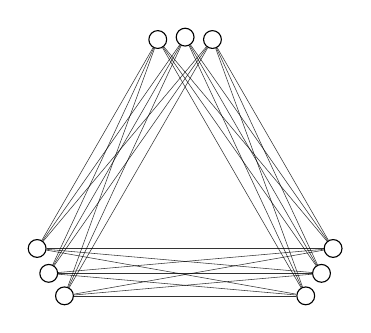
\begin{tikzpicture}[every node/.style=node]
            \node (a1) at ( 80:2) {};
            \node (a2) at ( 90:2) {};
            \node (a3) at (100:2) {};
            \node (b1) at (-20:2) {};
            \node (b2) at (-30:2) {};
            \node (b3) at (-40:2) {};
            \node (c1) at (200:2) {};
            \node (c2) at (210:2) {};
            \node (c3) at (220:2) {};
            \foreach \x in {1,2,3}
                \foreach \y in {1,2,3}{
                    \draw[very thin, opacity=0.8] (a\x) -- (b\y);
                    \draw[very thin, opacity=0.8] (a\x) -- (c\y);
                    \draw[very thin, opacity=0.8] (b\x) -- (c\y);
            }
        \end{tikzpicture}
    \end{center}
\end{fact}

\begin{defi}[Complete $r$-partite graph]\hypertarget{def:krt}
    Write $K_r(t)$ for the \textbf{complete $r$-partite graph} with $t$ vertices in each class (so $K_r(t) = \hyperlink{def:turan}{T_r(rt)}$).
\end{defi}

\begin{nthm}[Erd\H{o}s-Stone Theorem]\label{thm:14}
    Let $r, t \geq 1$ be integers, and let $\epsilon > 0$ be real.
    Then $\exists n_0$ such that $\forall n \geq n_0$,
    \begin{equation*}
        \abs{G} = n,\ \hyperlink{def:eG}{e(G)} \geq \left(1 - \frac{1}{r} + \epsilon\right) \binom{n}{2} \implies \hyperlink{def:krt}{K_{r+1}(t)} \subset G.
    \end{equation*}
\end{nthm}

\begin{proof}
    Coming up in \cref{sec:es}, non-examinable.
\end{proof}

This is enough to determine $\hyperlink{def:ex}{\ext}(H)$ for all $H$.

\begin{defi}[Chromatic number]\hypertarget{def:chromNum}
    If $H$ is a \hyperlink{def:graph}{graph}, the \textbf{chromatic number} of $H$, denoted $\chi(H)$, is the least $r$ such that $H$ is \hyperlink{def:rpartite}{$r$-partite}.
\end{defi}

\begin{eg}
    $\hyperlink{def:chromNum}{\chi}(\hyperlink{def:krt}{K_r(t)}) = r$.
\end{eg}

\begin{ncor}\label{cor:15}
    Let $H$ be a \hyperlink{def:graph}{graph} with at least one edge. Then
    \begin{equation*}
        \hyperlink{def:ex}{\ext(H)} = 1 - \frac{1}{\hyperlink{def:chromNum}{\chi(H)} - 1}.
    \end{equation*}
\end{ncor}

\begin{proof}
    Let $r = \hyperlink{def:chromNum}{\chi(H)} - 1$.
    Then $H$ is \hyperlink{def:rpartite}{$(r+1)$-partite} so we can find $t$ such that $H \subset \hyperlink{def:krt}{K_{r+1}(t)}$ (for instance $t = \abs{H}$ suffices).
    Let $\epsilon > 0$, and take $n_0$ as in \cref{thm:14}.
    Then for all $n \geq n_0$,
    \begin{align*}
        \abs{G} = n, \ e(G) \geq \left(1 - \frac{1}{r} + \epsilon\right) \binom{n}{2} &\implies K_{r+1}(t) \subset G \\
                                                                           &\implies H \subset G.
    \end{align*}
    So, for all $n \geq n_0$, $\hyperlink{def:exn}{\ext(n; H)} < (1 + \frac{1}{r} + \epsilon) \binom{n}{2}$. Hence
    \begin{equation*}
        \hyperlink{def:ex}{\ext(H)} = \lim_{n \to \infty} \frac{\ext(n; H)}{\binom{n}{2}} \leq 1 - \frac{1}{r} + \epsilon.
    \end{equation*}
    But $\epsilon>0$ was arbitrary, so $\ext(H) \leq 1 - \frac{1}{r}$.

    On the other hand, for all $n$, $H \not\subset \hyperlink{def:turan}{T_r(n)}$ as $H$ is not $r$-partite. So $\ext(n, H) \geq \hyperlink{def:turan}{t_r(n)}$, and
    \begin{equation*}
        \frac{t_r(n)}{\binom{n}{2}} \to 1 - \frac{1}{r} \quad \text{so} \quad \ext(H) \geq 1 - \frac{1}{r}. \qedhere
    \end{equation*}
\end{proof}

So if $H$ not \hyperlink{def:bipartite}{bipartite}, $\hyperlink{def:ex}{\ext}(H) = 1 - \frac{1}{\hyperlink{def:chromNum}{\chi(H)} - 1} \neq 0$, and $\hyperlink{def:exn}{\ext}(n; H) \hyperlink{def:asymp}{\sim} (1 - \frac{1}{\chi(H) - 1}) \binom{n}{2}$.
This essentially solves the forbidden subgraph problem for non-bipartite $H$.

What about if $H$ bipartite?
\Cref{cor:15} just says $\hyperlink{def:ex}{\ext}(H) = 0$, i.e. $\hyperlink{def:exn}{\ext}(n; H) = \hyperlink{def:asymp}{o(n^2)}$, but doesn't tell us for instance that $\ext(n; H)$ grows like a certain power of $n$.
We do however have upper bounds from \cref{thm:11}: $\ext(n, \hyperlink{def:knn}{K_{t, t}}) = \hyperlink{def:asymp}{\mathcal{O}}(n^{2 - \frac{1}{t}})$.

Another application of Erd\H{o}s-Stone:
\begin{defi}[Density]\hypertarget{def:density}
    We can define the \textbf{density} of a graph $G$ to be
    \begin{equation*}
        D(G) = \frac{\hyperlink{def:eG}{e(G)}}{\binom{\hyperlink{def:order}{\abs{G}}}{2}} \in [0, 1].
    \end{equation*}
\end{defi}

\begin{eg}
    \leavevmode
    \begin{itemize}
        \item $\hyperlink{def:density}{D}(\hyperlink{def:turan}{T_r(n)}) \to 1 - \frac{1}{r}$ as $n \to \infty$
        \item If $\alpha > \hyperlink{def:ex}{\ext(H)}$ then if $\abs{G}$ is sufficiently large and $D(G) = \alpha$, we have $H \subset G$.
    \end{itemize}
\end{eg}

Could we define the \hyperlink{def:density}{density} of an \hyperlink{def:infGraph}{infinite graph}?
We cannot take the same definition, as we would get $\frac{\infty}{\infty}$.
Instead try something like the `limit of densities of large finite subgraphs'.

\begin{defi}[Upper density]\hypertarget{def:ud}
    The upper density of an infinite graph $G$ is
    \begin{equation*}
        \ud(G) = \lim_{n \to \infty} \sup\set{\hyperlink{def:density}{D}(H) | H \subset G, \hyperlink{def:order}{\abs{H}} = n}.
    \end{equation*}
\end{defi}

\begin{remark}
    \leavevmode
    \begin{itemize}
        \item Again $\hyperlink{def:ud}{\ud}(G) \in [0, 1]$.
        \item If $\alpha < \ud(G)$ then for sufficiently large $n$, $G$ has subgraphs of order $n$ and \hyperlink{def:density}{density} $\geq \alpha$.
        \item If $\alpha > \ud(G)$ then for sufficiently large $n$, $G$ has no subgraphs of order $n$ and density $\geq \alpha$.
        \item A priori, it seems like $\ud(G)$ could take any value in $[0, 1]$. But surprisingly:
    \end{itemize}
\end{remark}

\begin{ncor}
    For any \hyperlink{def:infGraph}{infinite} graph $G$,
    \begin{equation*}
        \hyperlink{def:ud}{\ud}(G) \in \left\{0, 1, \frac{1}{2}, \frac{2}{3}, \frac{3}{4}, \dotsc\right\}.
    \end{equation*}
\end{ncor}

\begin{proof}
    It is enough to show that for $r = 1, 2, 3, \dotsc$,
    \begin{equation*}
        \hyperlink{def:ud}{\ud}(G) > 1 - \frac{1}{r} \implies \ud(G) \geq 1 - \frac{1}{r+1}.
    \end{equation*}
    Suppose $\ud(G) > 1 - \frac{1}{r}$.
    Pick $\alpha$ such that $\ud(G) > \alpha > 1 - \frac{1}{r}$ and fix $n$.
    For sufficiently large $N$, $G$ has subgraphs of order $N$ and density $\geq \alpha > 1 - \frac{1}{r} = \ext(\hyperlink{def:turan}{T_{r+1}(n)})$.
    So $T_{r+1}(n) \subset G$, but $D(T_{r+1}(n)) \to 1 - \frac{1}{r+1}$ as $n \to \infty$.
    We can do this for every $n$, hence $\ud(G) \geq 1 - \frac{1}{r+1}$.
\end{proof}

\subsubsection{Proof of Erd\H{o}s-Stone (non-examinable)}\label{sec:es}
We now return to prove the \nameref{thm:14}, which says that if a \hyperlink{def:graph}{graph} $G$ has enough edges, then $\hyperlink{def:krt}{K_{r+1}(t)} \subset G$.

This condition on $\hyperlink{def:eG}{e(G)}$ is equivalent to a condition on the \hyperlink{def:degree}{average degree}.
However, given $d$ and $\delta > 0$ then it turns out that any large graph of average degree $\geq d$ has a large subgraph of \hyperlink{def:degree}{minimum degree} $\geq d - \delta$.

If $G$ has average degree $d$ and $\hyperlink{def:order}{\abs{G}} = n$ large, we can find $\abs{H} = \hyperlink{def:asymp}{\Omega}(n)$ and $\hyperlink{def:degree}{\delta(H)} \geq d - \delta$ (not proved here. Delete vertices of minimum degree and it works).
So, we have an equivalent version of Erd\H{o}s-Stone with minimum degree condition:

\begin{manualtheorem}{14a}\label{thm:14a}
    Let $r, t \geq 1$ be integers and $\epsilon > 0$ be real. Then $\exists n_0$ such that $\forall n \geq n_0$,
    \begin{equation*}
        \hyperlink{def:order}{\abs{G}} = n, \quad \hyperlink{def:degree}{\delta(G)} \geq \left(1 - \frac{1}{r} + \epsilon\right) n \implies \hyperlink{def:krt}{K_{r+1}(t)} \subset G.
    \end{equation*}
\end{manualtheorem}

\begin{proof}
    Induction on $r$. Fix $T$ such that
    \begin{equation*}
        T > \left(\frac{2}{r\epsilon}\right)^t (t-1)
    \end{equation*}
    Then choose $n_0$ such that for all $n \geq n_0$,
    \begin{equation*}
        \abs{G} = n, \quad \hyperlink{def:degree}{\delta(G)} \geq \left(1 - \frac{1}{r} + \epsilon\right) n \implies \hyperlink{def:krt}{K_{r}(T)} \subset G.
    \end{equation*}
    (How? For $r=1$, $K_1(T) \subset G \iff \abs{G} \geq T$. For $r > 1$, $1 - \frac{1}{r} > 1 - \frac{1}{r-1}$ so it follows by inductive hypothesis.)

    Suppose the result is not true.
    Then we can find arbitrarily large $n$ and graphs $G$ with $\abs{G} = n$ and $\delta(G) \geq (1 - \frac{1}{r} + \epsilon) n$, $K_{r+1}(t) \not\subset G$.
    Pick such an $n$, $G$ with $n \geq n_0$ and also $n \geq \frac{2t}{r \epsilon}$.

    Then we can find $K_r(T) \subset G$, say with vertex classes $X_1, \dotsc, X_r$.
    \begin{center}
        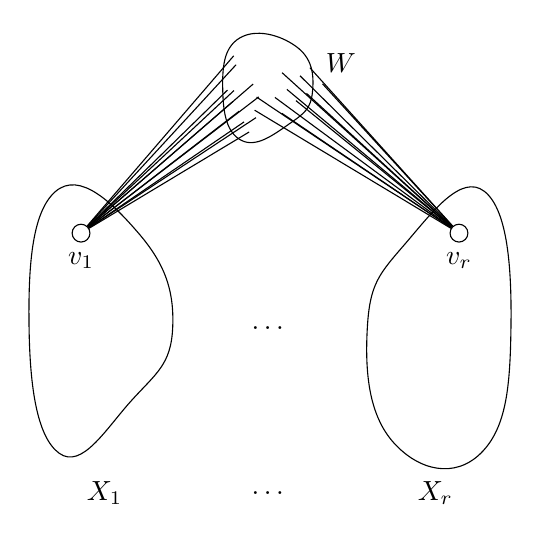
\begin{tikzpicture}[scale=0.6]
            \node [node,label=below:$v_1$] (a) at ( -4,  2) {};
            \node [node,label=below:$v_r$] (b) at (  4,  2) {};

            \foreach \theta in {10, 8, ..., -10}{
                \pgfmathsetmacro\randb{rand}
                \pgfmathsetmacro\randd{rand}

                \draw  (a) -- ++(\theta*0.8 + \randb*1.4 +  40 : 4.5 + \randb*0.5);
                \draw  (b) -- ++(\theta*0.8 + \randd*1.4 + 140 : 4.7 + \randd*0.5);
            }

            \draw plot [smooth cycle, tension=0.8, yshift=5cm] coordinates {(-180:1.0) (-120:1.2) (-60:0.8) (0:0.9) (60:1.1) (120:1.3)};
            \draw plot [smooth cycle, tension=0.8, xshift=-3.5cm, yscale=1.6, scale=1.6] coordinates {(-180:1.0) (-120:1.2) (-60:0.7) (0:0.9) (60:0.9) (120:1.3)};
            \draw plot [smooth cycle, tension=0.8, xshift=3.5cm, yscale=1.6, scale=-1.6] coordinates {(-180:1.0) (-120:1.3) (-60:0.8) (0:0.9) (60:1.1) (120:1.2)};

            \node at (1.5,5.6) {$W$};
            \node at (-3.5, -3.5) {$X_1$};
            \node at (0, -3.5) {$\dots$};
            \node at (0, 0) {$\dots$};
            \node at (3.5, -3.5) {$X_r$};
        \end{tikzpicture}
    \end{center}
    Let
    \begin{align*}
        A = \Set{(W, v_1, \dotsc, v_r) | W \subset \hyperlink{def:order}{V(G)}, \hyperlink{def:order}{\abs{W}} = t, \forall i\ v_i \in X_i, \forall i \forall w \in W: v_i \hyperlink{def:neighbour}{\sim} w}
    \end{align*}

    What can we say about $\abs{A}$?
    First, given $v_1 \in X, \dotsc, v_r \in X_r$, we can check from the minimum degree condition that
    \begin{equation*}
        \abs{\hyperlink{def:neighbour}{\Gamma}(v_1) \cap \dotsc \cap \Gamma(v_r)} \geq r \epsilon n
    \end{equation*}
    So there are at least $\binom{r \epsilon n}{t}$ choices for $W$. Hence $\abs{A} \geq T^r \binom{r \epsilon n}{t}$.

    On the other hand given the set $W$, as $K_{r+1}(t) \not\subset G$, we know that there is some $X_i$ containing at most $t-1$ vertices joined to all of $W$.
    Hence $\abs{A} \leq \binom{n}{t} (t-1) T^{r-1}$, thus
    \begin{equation*}
        T^r \binom{r \epsilon n}{t} \leq \binom{n}{t} (t-1) T^{r-1}.
    \end{equation*}
    Now,
    \begin{equation*}
        \text{RHS} \leq \frac{n^t}{t!} (t-1) T^{r-1}
    \end{equation*}
    while
    \begin{equation*}
        \text{LHS} \geq T^r \frac{1}{t!} (r \epsilon n - t)^t \geq T^r \frac{1}{t!} \left(\frac{r \epsilon n}{2}\right)^t.
    \end{equation*}
    Combining, we get
    \begin{equation*}
        T^r \left(\frac{r \epsilon n}{2}\right)^t \leq n^t (t-1) T^{r-1}
    \end{equation*}
    hence $T \leq (\frac{2}{r \epsilon})^t (t-1)$, a contradiction.
\end{proof}

\subsection{Hamiltonian graphs}
\begin{defi}[Hamiltonian]\hypertarget{def:hamil}
    A \textbf{Hamiltonian cycle} in a \hyperlink{def:graph}{graph} $G$ is a \hyperlink{def:cycle}{cycle} of length $G$, i.e.\ going through all vertices of $G$.
    If $G$ has a Hamiltonian cycle, we say $G$ is \textbf{Hamiltonian}.
\end{defi}
If $\hyperlink{def:order}{\abs{G}} = n$, how big does $e(G)$ need to be to force $G$ \hyperlink{def:hamil}{Hamiltonian}?
This turns out to be uninteresting, we can have $e(G)$ almost $\binom{n}{2}$ and have no Hamiltonian cycle.
\begin{center}
    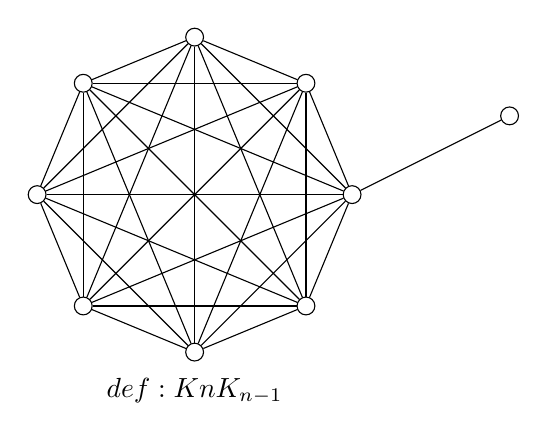
\begin{tikzpicture}
        \foreach \k in {0,...,7} {
            \node [node] (\k) at (360/8*\k+90:2) {};
        }
        \foreach \x in {0,...,7} {
            \foreach \y in {0,...,7} {
                \ifnum \x<\y
                    \draw (\x) -- (\y);
                \fi
            }
        }
        \node[node] (8) at (4, 1) {};
        \draw (6) -- (8);
        \node at (0, -2.5) {$\hyperlink{def:Kn}{K_{n-1}}$};
    \end{tikzpicture}
\end{center}

More interestingly then, is there a condition on $\hyperlink{def:degree}{\delta(G)}$?

\begin{nthm}[Dirac's Theorem]\label{thm:17}
    Let $\hyperlink{def:degree}{\abs{G}} = n \geq 3$ and $\hyperlink{def:degree}{\delta(G)} \geq \frac{n}{2}$. Then $G$ is \hyperlink{def:hamil}{Hamiltonian}.
\end{nthm}

\begin{remark}
    \leavevmode
    \begin{enumerate}[label=\arabic*.]
        \item This result is best possible:
            \begin{center}
                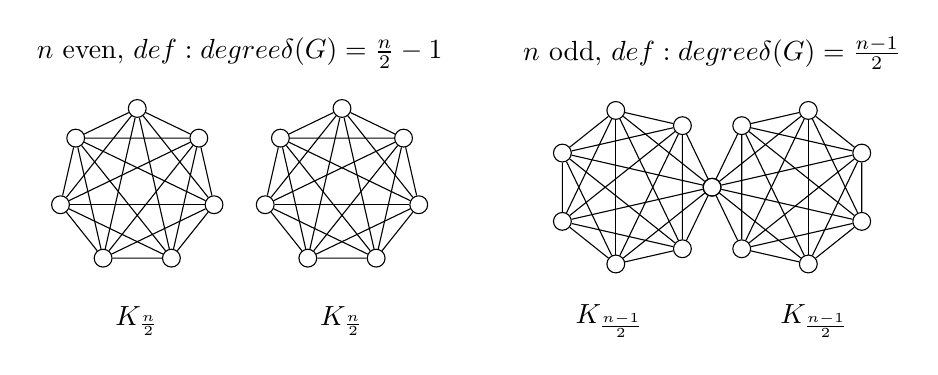
\begin{tikzpicture}
                    \begin{scope}
                        \node at (0,1.7) {$n$ even, $\hyperlink{def:degree}{\delta(G)} = \frac{n}{2}-1$};

                        \foreach \k in {0,...,6} {
                            \node [node,xshift=-1.3cm] (\k) at (360/7*\k+90:1) {};
                            \node [node,xshift= 1.3cm] (\k2) at (360/7*\k+90:1) {};
                        }
                        \foreach \x in {0,...,6} {
                            \foreach \y in {0,...,6} {
                                \ifnum \x<\y
                                    \draw (\x) -- (\y);
                                    \draw (\x2) -- (\y2);
                                \fi
                            }
                        }

                        \node at (-1.3,-1.7) {$K_{\frac{n}{2}}$};
                        \node at ( 1.3,-1.7) {$K_{\frac{n}{2}}$};
                    \end{scope}
                    \begin{scope}[xshift=6cm]
                        \node at (0,1.7) {$n$ odd, $\hyperlink{def:degree}{\delta(G)} = \frac{n-1}{2}$};

                        \foreach \k in {0,...,6} {
                            \node [node,xshift=-1cm] (\k) at (360/7*\k:1) {};
                            \node [node,xshift= 1cm] (\k2) at (360/7*\k-180:1) {};
                        }
                        \foreach \x in {0,...,6} {
                            \foreach \y in {0,...,6} {
                                \ifnum \x<\y
                                    \draw (\x) -- (\y);
                                    \draw (\x2) -- (\y2);
                                \fi}}
                        \node at (-1.3,-1.7) {$K_{\frac{n-1}{2}}$};
                        \node at ( 1.3,-1.7) {$K_{\frac{n-1}{2}}$};
                    \end{scope}
                \end{tikzpicture}
            \end{center}
        \item Of course there are \hyperlink{def:hamil}{Hamiltonian} graphs of smaller minimum degree:
            \begin{center}
                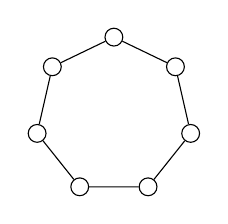
\begin{tikzpicture}[every node/.style=node]
                    \foreach \k in {0,...,6} {
                        \node [node,xshift=-1cm] (\k) at (360/7*\k+90:1) {};
                    }
                    \draw (0) -- (1) -- (2) -- (3) -- (4) -- (5) -- (6) -- (0);
                \end{tikzpicture}
            \end{center}
        \item In general, given a graph $G$ it is hard computationally to determine if $G$ has a Hamiltonian cycle.
    \end{enumerate}
\end{remark}

\begin{proof}
    First, observe $G$ is \hyperlink{def:components}{connected}.
    Indeed, if $x \neq y$, $x \hyperlink{def:neighbour}{\nsim} y$, then $\abs{\hyperlink{def:neighbour}{\Gamma}(x) \cup \Gamma(y)} \leq n-2$, but $\abs{\Gamma(x)} + \abs{\Gamma(y)} \geq \frac{n}{2} + \frac{n}{2} = n$ so $\Gamma(x) \cap \Gamma(y) \neq \emptyset$.

    Let $v_0, v_1, \dotsc, v_k$ be a \hyperlink{def:path}{path} of maximal length in $G$, say length $k \leq n-1$.
    By maximality, $\Gamma(v_0) \subset \{v_1, \dotsc, v_k\}$. Similarly, $\Gamma(v_k) \subset \{v_0, \dotsc, v_{k-1}\}$.
    \begin{center}
        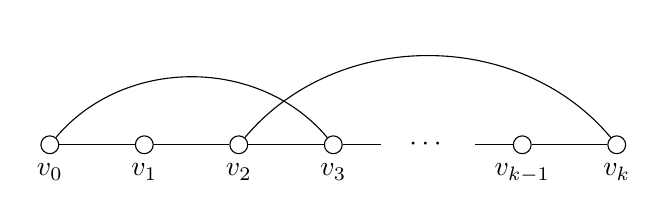
\begin{tikzpicture}[scale=1.2]
            \node [node, label=below:$v_0$]     (0) at (  0,  0)  {};
            \node [node, label=below:$v_1$]     (1) at (  1,  0)  {};
            \node [node, label=below:$v_2$]     (2) at (  2,  0)  {};
            \node [node, label=below:$v_3$]     (3) at (  3,  0)  {};

            \node [node, label=below:$v_{k-1}$] (4) at (  5,  0)  {};
            \node [node, label=below:$v_k$]     (5) at (  6,  0)  {};

            \node [draw=none] at (4, 0) {$\cdots$};
            \draw (0) -- (1) -- (2) -- (3) -- (3.5, 0);
            \draw (4.5, 0) -- (4) -- (5);
            \draw (0) to[bend left=50] (3);
            \draw (2) to[bend left=50] (5);
        \end{tikzpicture}
    \end{center}

    If we have some situation like in the diagram, we get a \hyperlink{def:cycle}{cycle}. To be more precise, if
    \begin{equation*}
        A = \set{i \in [k] | v_0 \sim v_i} \quad \text{and} \quad B = \set{i \in [k] | v_k \sim v_{i-1}}
    \end{equation*}
    then $A \cap B \neq \emptyset \implies$ we have a cycle.
    But $\abs{A \cup B} \leq k < n$ while $\abs{A} + \abs{B} \geq \frac{n}{2} + \frac{n}{2} = n$.
    Hence $\exists i \in A \cap B$ so we have a cycle $C = v_0 v_1 \dotsc v_{i-1} v_k v_{k-1} \dotsc v_i v_0$ of length $k+1$.

    If $k = n-1$, we have a \hyperlink{def:hamil}{Hamiltonian} cycle as required.
    If $k < n-1$, relabel the cycle $C = u_0 u_1 \dotsc u_k u_0$.
    By connectedness, we have some $u_i \in C$ and $w \notin C$ with $w \sim u_i$.
    Then $w u_i u_{i+1} \dotsc u_k u_0 \dotsc u_{i-1}$ is a path of length $k+1$, contradicting maximality.
\end{proof}

\begin{remark}
    The same proof gives the following:
    Let $n > k \geq 3$ and let $G$ be a \hyperlink{def:components}{connected} \hyperlink{def:graph}{graph} $\hyperlink{def:order}{\abs{G}} = n$ with $\hyperlink{def:degree}{\delta(G)} \geq \frac{k}{2}$.
    Then $G$ contains a \hyperlink{def:path}{path} of length $k$ and a \hyperlink{def:cycle}{cycle} of length at least $\frac{k+2}{2}$.
\end{remark}

The \hyperlink{def:konig}{Konigsberg bridge problem} seems superficially similar, but in fact is much less interesting.
\begin{defi}[Euler circuit]\hypertarget{def:euler}
    A \textbf{circuit} of a \hyperlink{def:graph}{graph} $G$ is a sequence $v_0 v_1 \dotsc v_n$ of vertices of $G$, not necessarily distinct with $v_0 = v_n$, where if $1 \leq i \leq k$ then $v_{i-1} \hyperlink{def:neighbour}{\sim} v_i$ and if $1 \leq i < j \leq k$ then edges $v_{i-1} v_i$ and $v_{j-1} v_j$ are distinct.
    It is an \textbf{Euler circuit} if for every $e \in \hyperlink{def:eG}{E(G)}$, there is some $i$ with $e = v_{i-1} v_i$.
    If $G$ has an Euler circuit we say $G$ is \textbf{Eulerian}.
\end{defi}

We are only interested in \hyperlink{def:components}{connected} graphs: We could have a non-connected \hyperlink{def:euler}{Eulerian} graph, but only because of the \hyperlink{def:degree}{degree} zero vertices.
\begin{center}
    \begin{tikzpicture}
        \node [node] (A) at (  90:1)  {};
        \node [node] (B) at (-150:1)  {};
        \node [node] (C) at ( -30:1)  {};

        \draw (A) -- (B) -- (C) -- (A);
        \node [node] at (2,0.3) {};
        \node [node] at (3.3,0.3) {};
    \end{tikzpicture}
\end{center}

\begin{nprop}\label{thm:18}
    Let $G$ be a \hyperlink{def:components}{connected} \hyperlink{def:graph}{graph}. Then
    \begin{equation*}
        G\text{ \hyperlink{def:euler}{Eulerian} if and only if } \forall v \in G,\ \hyperlink{def:degree}{d(v)}\text{ is even.}
    \end{equation*}
\end{nprop}

\begin{proof}
    ($\Rightarrow$) is obvious: an \hyperlink{def:euler}{Eulerian circuit} must go in and out of a given vertex the same number of times.

    ($\Leftarrow$): use induction on $\hyperlink{def:eG}{e(G)}$. For $e(G) = 0$ it is clearly true.

    Consider $e(G) > 0$. Let $v_0 v_1 \dotsc v_k = C$ be a \hyperlink{def:euler}{circuit} in $G$ of maximal length.
    If $C$ uses all edges of $G$ then we are done.
    If not, delete all edges used in $C$ from $G$ to form $H$.
    In $H$, every vertex still has even degree. Let $H_1$ be a \hyperlink{def:components}{component} of $H$ with at least one edge.

    By induction hypothesis, $H_1$ has an Euler circuit $D$.
    Certainly $C, D$ meet at some vertex $v$.
    Join them at $v$ to produce a longer circuit in $G$, a contradiction.
    (Walk along $C$ until we get to $v$, then walk all round $D$ starting/ending at $v$, then walk along the rest of $C$).
\end{proof}

\clearpage
\section{Graph Colouring}
Think about the map-colouring problem.
How many colours do we need to colour graphs with no crossings, such that adjacent vertices have different colours.

\begin{defi}[Colouring]\hypertarget{def:colour}
    A \textbf{$k$-colouring} of a \hyperlink{def:graph}{graph} $G$ is a function $c: V(G) \to [k]$.
    In proofs we often say \red{`red'}, \green{`green'} for 1,2, etc.
\end{defi}
Note $G$ has a \hyperlink{def:colour}{$k$-colouring} if and only if $G$ is \hyperlink{def:rpartite}{$k$-partite}.
So, $\hyperlink{def:chromNum}{\chi(G)}$ is the least number of colours needed to colour $G$.

\subsection{Planar Graphs}
\begin{defi}[Graph drawing]\hypertarget{def:drawing}
    A \textbf{drawing} of $G$ is an ordered pair $(f, \gamma)$ where $f: V \to \R^2$ is an injection and $\gamma: E \to C([0, 1], \R^2)$ such that
    \begin{enumerate}[label=(\roman*)]
        \item If $uv \in E$ then $\{\gamma(uv)(0), \gamma(uv)(1)\} = \{f(u), f(v)\}$.
        \item If $e, e' \in E$ with $e \neq e'$ then $\gamma(e)((0, 1)) \cap \gamma(e')((0,1)) = \emptyset$.
        \item If $e \in E$ then $\gamma(e)$ is injective.
        \item If $e \in E$ and $v \in V$ then $f(v) \notin \gamma(e)((0, 1))$
    \end{enumerate}
    That is,
    \begin{align*}
        \text{vertices} &\longleftrightarrow \text{points} \\
        \text{edges} &\longleftrightarrow \text{continuous curves between end vertices},
    \end{align*}
    with no unnecessary intersections.
    If $G$ has a drawing, we say $G$ is \textbf{planar}.
\end{defi}

Are there topological problems? Perhaps an edge is represented by a space-filling curve.
But,
\begin{fact}
    Any \hyperlink{def:drawing}{planar} graph can be drawn with piecewise linear edges - i.e.\ each edge is finitely many line segments.
    Henceforth, assume all drawings satisfy this.
\end{fact}

\begin{eg}
    \leavevmode
    \begin{enumerate}[label=\arabic*.]
        \item \hyperlink{def:Kn}{$K_3$} is \hyperlink{def:drawing}{planar}
            \begin{center}
                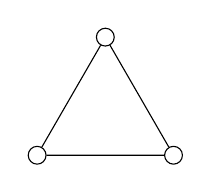
\begin{tikzpicture}
                    \node [node] (A) at (  90:1)  {};
                    \node [node] (B) at (-150:1)  {};
                    \node [node] (C) at ( -30:1)  {};

                    \draw (A) -- (B) -- (C) -- (A);
                \end{tikzpicture}
            \end{center}
        \item $K_4$ may appear non-planar but it is in fact planar.
            \begin{center}
                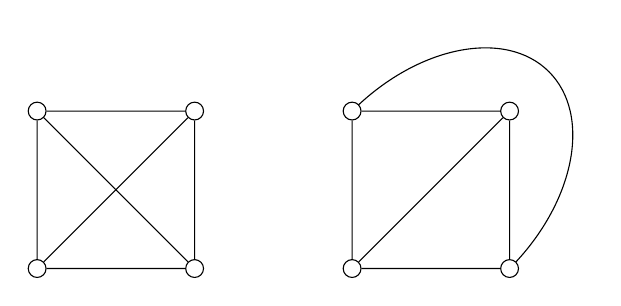
\begin{tikzpicture}
                    \begin{scope}
                        \node [node] (A) at ( 1, 1)  {};
                        \node [node] (B) at (-1, 1)  {};
                        \node [node] (C) at (-1,-1)  {};
                        \node [node] (D) at ( 1,-1)  {};

                        \draw (A) -- (B) -- (C) -- (D) -- (A) -- (C);
                        \draw (B) -- (D);
                    \end{scope}
                    \begin{scope}[xshift=4cm]
                        \draw [rotate=45] (0,1.414) arc [x radius=2.121cm, y radius=1.414cm, start angle=90, end angle=-90];
                        \node [node,fill=white] (A) at ( 1, 1)  {};
                        \node [node,fill=white] (B) at (-1, 1)  {};
                        \node [node,fill=white] (C) at (-1,-1)  {};
                        \node [node,fill=white] (D) at ( 1,-1)  {};

                        \draw (A) -- (B) -- (C) -- (D) -- (A) -- (C);
                    \end{scope}
                \end{tikzpicture}
            \end{center}
        \item $K_5$ is not planar.
            \begin{center}
                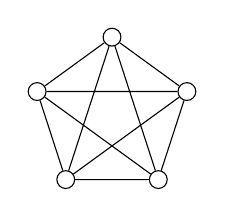
\begin{tikzpicture}
                    \begin{scope}[xshift=2cm,yshift=0.3cm]
                        \node [node] (A) at (  90:1)  {};
                        \node [node] (B) at ( 162:1)  {};
                        \node [node] (C) at (-126:1)  {};
                        \node [node] (D) at ( -54:1)  {};
                        \node [node] (E) at (  18:1)  {};

                        \draw (A) -- (B) -- (C) -- (D) -- (E) -- (A);
                        \draw (A) -- (C) -- (E) -- (B) -- (D) -- (A);
                    \end{scope}
                \end{tikzpicture}
            \end{center}

            Suppose we have a drawing of $K_5$.
            It must contain a closed curve, say through vertices $u, v, w, x, y$ in that order.
            The curve divides the plane into inside and outside.
            \begin{center}
                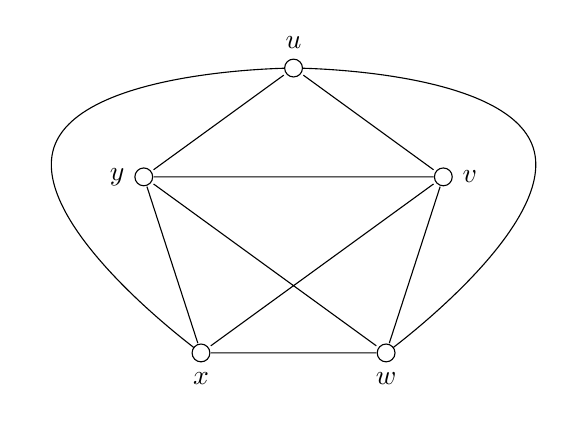
\begin{tikzpicture}[scale=2]
                    \node (u) at (  90:1)  {};
                    \node (y) at ( 162:1)  {};
                    \node (x) at (-126:1)  {};
                    \node (w) at ( -54:1)  {};
                    \node (v) at (  18:1)  {};

                    \draw (u) to (v) to (w) to (x) to (y) to (u);
                    \draw (x) to (v) to (y) to (w);
                    \draw plot [smooth,tension=1] coordinates {(u) (162:1.6) (x)};
                    \draw plot [smooth,tension=1] coordinates {(u) (18:1.6) (w)};

                    \node [node,label=above:$u$,fill=white] at (u) {};
                    \node [node,label=left: $y$,fill=white] at (y) {};
                    \node [node,label=below:$x$,fill=white] at (x) {};
                    \node [node,label=below:$w$,fill=white] at (w) {};
                    \node [node,label=right:$v$,fill=white] at (v) {};
                \end{tikzpicture}
            \end{center}
            Suppose edge $vy$ is inside. Then $ux, uw$ are outside.
            So $yu$, $vx$ inside, so they intersect, a contradiction.
            Similarly, we can show $vy$ cannot be outside, hence $K_5$ is not planar.
        \item $\hyperlink{def:knn}{K_{3,3}}$ is not planar by similar argument (exercise).
    \end{enumerate}
\end{eg}

Clearly if $\hyperlink{def:Kn}{K_5} \subset G$ or $\hyperlink{def:knn}{K_{3,3}} \subset G$ then $G$ is not \hyperlink{def:drawing}{planar}.
Remarkably, these are the only obstacles to planarity.
Also, e.g.\
\begin{center}
    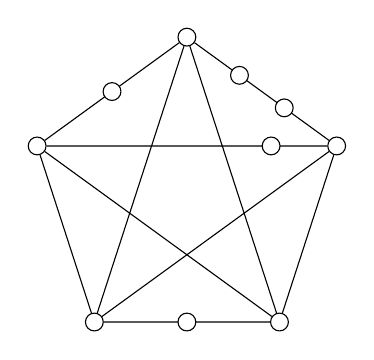
\begin{tikzpicture}[scale=2]
        \begin{scope}
            \node [node] (A) at (  90:1)  {};
            \node [node] (B) at ( 162:1)  {};
            \node [node] (C) at (-126:1)  {};
            \node [node] (D) at ( -54:1)  {};
            \node [node] (E) at (  18:1)  {};

            \draw (A) -- node[node, pos=0.5,fill=white] {} (B) -- (C) -- node[node, pos=0.5,fill=white] {} (D) -- (E) -- node[node, pos=0.333,fill=white] {} node[node, pos=0.666,fill=white] {} (A);
            \draw (A) -- (C) -- (E) -- node[node, pos=0.2,fill=white] {} (B) -- (D) -- (A);
        \end{scope}
    \end{tikzpicture}
\end{center}

\begin{defi}[Subdivision]\hypertarget{def:subdiv}
    Let $G$ be a \hyperlink{def:graph}{graph}.
    A \textbf{subdivision} of $G$ is a graph formed by repeatedly selecting $vw \in \hyperlink{def:eG}{E(G)}$, removing $vw$ and adding vertex $u$ and edges $uv, uw$.
\end{defi}

\begin{nthm}[Kuratowski's Theorem]\label{thm:19}
    Let $G$ be a \hyperlink{def:graph}{graph}. Then $G$ \hyperlink{def:drawing}{planar} iff $G$ contains no \hyperlink{def:subdiv}{subdivision} of \hyperlink{def:Kn}{$K_5$} or \hyperlink{def:knn}{$K_{3,3}$}.
\end{nthm}

Recall that a \hyperlink{def:tree}{tree} is a \hyperlink{def:components}{connected} \hyperlink{def:cycle}{acyclic} \hyperlink{def:graph}{graph}.
\begin{defi}[Leaf]\hypertarget{def:leaf}
    A \textbf{leaf} of a \hyperlink{def:tree}{tree} is a vertex of order 1.
\end{defi}

\begin{nprop}\label{prop:20}
    Every \hyperlink{def:tree}{tree} of \hyperlink{def:order}{order} at least $2$ has a \hyperlink{def:leaf}{leaf}.
\end{nprop}

\begin{proof}
    Let $T$ be a \hyperlink{def:tree}{tree} $\hyperlink{def:order}{\abs{T}} \geq 2$ and let $v_0 v_1 \dotsc v_k$ be a \hyperlink{def:path}{path} of maximum length in $T$.
    Now $v_k \hyperlink{def:neighbour}{\sim} v_{k-1}$, but $v_k$ has no other neighbours in the path (as $T$ \hyperlink{def:cycle}{acyclic}) and $v_k$ has no neighbours outside path (by maximality).
    Hence $v_k$ is a \hyperlink{def:leaf}{leaf}.
\end{proof}

Why do we care? If $T$ is a \hyperlink{def:tree}{tree}, $\hyperlink{def:order}{\abs{T}} \geq 2$, then $T$ has a \hyperlink{def:leaf}{leaf} $v$ and $T-v$ is a tree of smaller order.
This is particularly useful for induction, for instance

\begin{nprop}\label{prop:21}
    Let $T$ be a \hyperlink{def:tree}{tree}, $\hyperlink{def:order}{\abs{T}} = n \geq 1$. Then $\hyperlink{def:eG}{e(T)} = n-1$.
\end{nprop}

\begin{proof}
    Use induction on $n$. For $n=1$, $\hyperlink{def:eG}{e(T)} = 0$ as required.

    For $n > 1$, let $v$ be a \hyperlink{def:leaf}{leaf}.
    Then $T - v$ is a \hyperlink{def:tree}{tree} with $\hyperlink{def:order}{\abs{T - v}} = n-1$ so by the induction hypothesis, $e(T-v) = n-2$, so $e(T) = n-1$.
\end{proof}

\begin{nprop}\label{prop:22}
    Every \hyperlink{def:tree}{tree} is \hyperlink{def:drawing}{planar}.
\end{nprop}

\begin{proof}
    Let $T$ be a \hyperlink{def:tree}{tree}, $\hyperlink{def:order}{\abs{T}} = n$ and use induction on $n$.
    For $n=0,1$ we are done immediately.

    For $n > 1$, let $v \in T$ be a \hyperlink{def:leaf}{leaf}.
    By the induction hypothesis, $T-v$ can be \hyperlink{def:drawing}{drawn}.
    Let $u \in T$ be the \hyperlink{def:neighbour}{neighbour} of $v$.
    Take a small circle around $u$ in the drawing; so the circle contains only the centre and some radii in the drawing.
    Hence, we can easily add $v$ and $uv$ to the drawing.
\end{proof}

\begin{defi}[Faces]\hypertarget{def:face}
    If we have a \hyperlink{def:drawing}{drawing} of a \hyperlink{def:graph}{graph}, it divides the plane into connected regions called \textbf{faces}. Precisely one of these regions, the \textbf{infinite face} is unbounded.
\end{defi}
\begin{remark}
    Important warning: \hyperlink{def:graph}{Graphs} don't have \hyperlink{def:face}{faces}, \hyperlink{def:drawing}{drawings} have faces.
\end{remark}

\begin{nthm}[Euler's Formula]\label{thm:23}
    Take $G$ \hyperlink{def:components}{connected} and \hyperlink{def:drawing}{planar}.
    Take $\hyperlink{def:order}{\abs{G}} = n \geq 1$, $\hyperlink{def:eG}{e(G)} = m$ with $l$ \hyperlink{def:face}{faces}.
    Then $n - m + l = 2$.
\end{nthm}

\begin{proof}
    Induction on $m$. If $G$ is a \hyperlink{def:tree}{tree:} $m = n-1$, $l = 1$, and we are done.

    Otherwise, $G$ has a \hyperlink{def:cycle}{cycle}.
    Pick an edge $e$ in the cycle and consider $G-e$. Then $\hyperlink{def:order}{\abs{G - e}} = n$, $\hyperlink{def:eG}{e(G-e)} = m-1$.
    Moreover, in our \hyperlink{def:drawing}{drawing}, removing $e$ combines two faces so we have drawn $G-e$ with $l-1$ faces.
    So, by the induction hypothesis $n - (m-1) + (l-1) = 2$, so $n - m + l = 2$.
\end{proof}

\begin{ncor}\label{cor:24}
    Let $G$ be \hyperlink{def:drawing}{planar}, $\hyperlink{def:order}{\abs{G}} = n \geq 3$. Then $\hyperlink{def:eG}{e(G)} \leq 3n-6$.
\end{ncor}

\begin{proof}
    Let $\hyperlink{def:eG}{e(G)} = m$. Draw $G$ with $l$ \hyperlink{def:face}{faces}.
    Without loss of generality, $G$ is \hyperlink{def:components}{connected} (if not, add edges to make it so).

    We have a special case where
    \begin{center}
        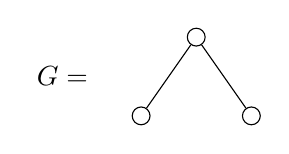
\begin{tikzpicture}
            \node at (-1,0) {$G=$};
            \node [node] (A) at (0  ,-0.5) {};
            \node [node] (B) at (0.7, 0.5) {};
            \node [node] (C) at (1.4,-0.5) {};
            \draw (A) -- (B) -- (C);
        \end{tikzpicture}
    \end{center}
    with $n = 3$, $m = 2$ and $3n-6 = 3 \geq 2$.

    Otherwise, we know $n - m + l = 2$ and each face has at least 3 edges in its boundary, and each edge is in the boundary of at most 2 faces.
    So, $l \leq \frac{2m}{3}$.
    Thus, $n -m + \frac{2}{3}m \geq 2$ so $\frac{1}{3}m \geq n-2$ so $m \geq 3n-6.$
\end{proof}

\begin{nprop}[Six colour theorem]\label{prop:25}
    Any \hyperlink{def:drawing}{planar} graph is 6-\hyperlink{def:colour}{colourable}.
\end{nprop}

\begin{proof}
    Let $G$ be \hyperlink{def:drawing}{planar}, $\hyperlink{def:order}{\abs{G}} = n$. Induction on $n$.
    For $n \leq 6$, give every vertex a different colour, as required.

    For $n > 6$, by \cref{cor:24}, $e(G) \leq 3n - 6$. Hence
    \begin{equation*}
        \hyperlink{def:degree}{\delta(G)} \leq \frac{2 \hyperlink{def:eG}{e(G)}}{\hyperlink{def:order}{\abs{G}}} \leq \frac{6n-12}{n} = 6 - \frac{12}{n} < 6.
    \end{equation*}
    So, $\delta(G) \leq 5$.

    Pick $v \in G$ with $d(v) \leq 5$. By inductive hypothesis, $G- v$ can be 6-\hyperlink{def:colour}{coloured}.
    Some colour is missing from $\hyperlink{def:neighbour}{\Gamma(v)}$, use this colour to colour $v$.
\end{proof}

A lot more work gives:
\begin{nthm}[Five colour theorem]\label{thm:26}
    Any \hyperlink{def:drawing}{planar} graph is 5-\hyperlink{def:colour}{colourable}.
\end{nthm}
\begin{proof}
    Let $G$ be \hyperlink{def:drawing}{planar}, $\hyperlink{def:order}{\abs{G}} = n$.
    Use induction on $n$.
    The base case $n\leq 5$ is trivial, so take $n > 5$.
    As in \cref{prop:25}, we can find $v \in G$ with $\hyperlink{def:degree}{\delta(v)} \leq 5$ and 5-\hyperlink{def:colour}{colour} $G-v$.
    If there is a colour missing from $\hyperlink{def:neighbour}{\Gamma(v)}$, use that colour at $v$.
    Otherwise, draw $G$; WLOG $v$ has neighbours $x_1, \dotsc, x_5$ in clockwise order around $v$ with colours $\green{1}, \red{2},\purple{3},\blue{4},\orange{5}$ respectively.

    \hypertarget{def:ijpath}Call a \hyperlink{def:path}{path} in $G-v$ an \textbf{$ij$-path} if all its vertices have colour $i$ or $j$.
    \hypertarget{def:ijcomp}Given $x \in G-v$, the \textbf{$ij$-component} of $x$ consists of those vertices reachable from $x$ along \hyperlink{def:ijpath}{$ij$-paths}.

    If $x_1, x_3$ are in different \hyperlink{def:ijcomp}{$\green{1}\purple{3}$ components}, then swap the colours of $1,3$ on the $\green{1}\purple{3}$ component of $x_1$ and give $v$ colour $\green{1}$.
    \begin{center}
        \begin{tikzpicture}[scale=2]
            \node [node,thick,        label=below:$v$]   (v) at (0,0)  {};
            \node [node,thick,bgreen   ,label=above:$x_1$] (x1) at ( 90:1) {};
            \node [node,thick,bred,label=right:$x_2$] (x2) at ( 18:1) {};
            \node [node,thick,bpurple  ,label=below:$x_3$] (x3) at (-54:1) {};
            \node [node,thick,bblue,label=below:$x_4$] (x4) at (-126:1) {};
            \node [node,thick,borange ,label=left :$x_5$] (x5) at (162:1) {};
            \begin{scope}[every node/.style={node,thick}]
                \node [bpurple] (y1) at (1,1.4) {};
                \node [bgreen]    (y2) at (2,1) {};
                \node [bpurple] (y3) at (2.1,0) {};
                \node [bgreen]    (y4) at (1.6,-0.8) {};
            \end{scope}
            \foreach \x in {1,...,5} { \draw (v) -- (x\x); }
            \draw (x1) -- (y1) -- (y2) -- (y3) -- (y4) -- (x3);
        \end{tikzpicture}
    \end{center}

    If not, then $x_2, x_4$ are in different $\red{2}\blue{4}$ components as we see in the diagram, so swap colours $2, 4$ on the $\red{2}\blue{4}$ component of $x_2$ and give $v$ colour $\red{2}$.
\end{proof}

\begin{nthm}[Four colour theorem]\label{thm:27}
    Any \hyperlink{def:drawing}{planar} graph is 4-\hyperlink{def:colour}{colourable}.
\end{nthm}

\begin{proof}
    Let $G$ be \hyperlink{def:drawing}{planar}, $\hyperlink{def:order}{\abs{G}} = n$ and use induction on $n$. For $n=4$, we are immediately done.

    For $n > 4$, pick $v \in G$ with $\hyperlink{def:degree}{d(v)} \leq 5$, then \hyperlink{def:drawing}{draw} $G$ and 4-\hyperlink{def:colour}{colour} $G-v$.
    If some colour is missing on $\Gamma(v)$ then we are done.
    If not, there are three cases.

    Case 1: $d(v) = 4$.
    There cannot be both a $\green{1}\purple{3}$-path from $x_1$ to $x_3$ and a $\red{2}\blue{4}$ path from $x_2$ to $x_4$, so done as in the proof of \cref{thm:26}.
    \begin{center}
        \begin{tikzpicture}[scale=2]
            \node [node,thick]   (v) at (0,0)  {};
            \node (x1) at (0,1) {};
            \node (x3) at (0,-1) {};
            \node [node,thick,bred,label=right:$x_2$] (x2) at (1,0) {};
            \node [node,thick,bblue,label=below:$x_4$] (x4) at (-1,0) {};
            \foreach \x in {1,...,4} {
                \draw (v) -- (x\x);
            }
            \draw plot [smooth, tension=1.6] coordinates {(x1) (2,0) (x3)};
            \node [node,thick,bgreen,fill=white,label=above:$x_1$] at (x1)  {};
            \node [node,thick,bpurple,fill=white,label=below:$x_3$] at (x3) {};
            \draw [->] (x2) to [bend left=10] (0.6,-0.4);
            \node at (0.5,-0.5) {$\times$};
        \end{tikzpicture}
    \end{center}

    Case 2: $d(v) = 5$, $v$ has neighbours $x_1, \dotsc, x_5$ clockwise with colours $\green{1},\red{2},\purple{3},\blue{4},\green{1}$.

    \begin{center}
        \begin{tikzpicture}[scale=2]
            \node [node,thick] (v) at (0,0) {};
            \node (x1) at ( 0.6,0.9) {};
            \node (x5) at (-0.6,0.9) {};
            \node (x2) at (1,0) {};
            \node (x3) at (0,-1) {};
            \node (x4) at (-1,0) {};
            \foreach \x in {1,...,5} {
                \draw (v) -- (x\x);
            }
            \draw plot [smooth, tension=1.6] coordinates {(x2) (0,-1.5) (x4)};
            \node [node,thick,bgreen, fill=white,label=above:$x_1$] at (x1) {};
            \node [node,thick,bgreen, fill=white,label=above:$x_5$] at (x5) {};
            \node [node,thick,bpurple,fill=white,label=below:$x_3$] at (x3) {};
            \node [node,thick,bred,   fill=white,label=right:$x_2$] at (x2) {};
            \node [node,thick,bblue,  fill=white,label=left :$x_4$] at (x4) {};
            \draw [->] (x3) to [bend left=10] (-0.4,-0.6);
            \node at (-0.5,-0.5) {$\times$};
        \end{tikzpicture}
    \end{center}
    Then there is either no $\red{2}\blue{4}$ path from $x_2$ to $x_4$ or no $\green{1}\purple{3}$ path from $x_3$ to $x_1$, so again we are done.

    Case 3: $d(v) = 5$, colours $\green{1},\red{2},\purple{3},\green{1},\blue{4}$.
    \begin{center}
        \begin{tikzpicture}[scale=2]
            \node [node,thick] (v) at (0,0) {};
            \node (x1) at (54:1) {};
            \node (x2) at (-18:1) {};
            \node (x3) at (-90:1) {};
            \node (x4) at (-162:1) {};
            \node (x5) at (126:1) {};
            \foreach \x in {1,...,5} {
                \draw (v) -- (x\x);
            }
            \draw plot [smooth, tension=1.6] coordinates {(x2) (54:1.5) (x5)};
            \draw plot [smooth, tension=1.6] coordinates {(x5) (-162:1.5) (x3)};

            \node [node,thick,bgreen, fill=white,label=above:$x_1$] at (x1) {};
            \node [node,thick,bred,   fill=white,label=right:$x_2$] at (x2) {};
            \node [node,thick,bpurple,fill=white,label=below:$x_3$] at (x3) {};
            \node [node,thick,bgreen, fill=white,label=left :$x_4$] at (x4) {};
            \node [node,thick,bblue,  fill=white,label=above:$x_5$] at (x5) {};
        \end{tikzpicture}
    \end{center}
    If there is no $\red{2}\blue{4}$ path from $x_2$ to $x_5$, we are done.
    If there is no $\purple{3}\blue{4}$ path from $x_3$ to $x_5$, we are done.

    Otherwise, swap colours $\green{1},\purple{3}$ on the $\green{1}\purple{3}$ component of $x_1$ and swap colours $\green{1},\red{2}$ on the $\green{1}\red{2}$ component of $x_4$.
    Then, use colour $\green{1}$ at $v$, but this is false.
\end{proof}

% new lec

The \Cref{thm:27} was proved correctly in 1976, with 1936 cases checked.

\subsection{General Graphs}
We know $G$ \hyperlink{def:drawing}{planar} $\Rightarrow \hyperlink{def:chromNum}{\chi(G)} \leq 4$.

What can we say about $\hyperlink{def:chromNum}{\chi(G)}$ if not given $G$ \hyperlink{def:drawing}{planar}?
Clearly $\chi(G)$ can be as large as we like, e.g. $\chi(\hyperlink{def:Kn}{K_k}) = k$.

\subsubsection*{Lower bounds}
\begin{enumerate}[label=(\alph*)]
    \item If $\hyperlink{def:Kn}{K_k} \subset G$ then $\hyperlink{def:chromNum}{\chi(G)} \geq k$.
        \hypertarget{def:cliqueNum}The \textbf{clique number} of $G$ is $\omega(G) = \max\set{k | K_k \subset G}$. Then $\chi(G) \leq \omega(G)$.
        Sometimes this bound is not good. For instance, we can find $G$ with $\omega(G) = 2$ and $\chi(G)$ arbitrarily large (see example sheet 2).
    \item Suppose we have a \hyperlink{def:colour}{colouring} of $G$.
        Let $W \subset V(G)$ be a colour class.
        \hypertarget{def:independentSet}Then $W$ is an \textbf{independent set} - there are no edges within $W$.
        \hypertarget{def:indepNum}The \textbf{independence number} of $G$ is
        \begin{equation*}
            \alpha(G) = \max\set{\abs{W} | W \subset V(G), W \text{ \hyperlink{def:independentSet}{independent}}}.
        \end{equation*}
        Then $\chi(G) \geq \frac{\abs{G}}{\alpha(G)}$.
        Sometimes this bound is not good.
        For instance, take $G = K_k \cup \overline{K_k}$.
        Then $\chi(G) = k$, $\frac{\abs{G}}{\alpha(G)} = \frac{2k}{k+1} \approx 2$.
        \begin{center}
            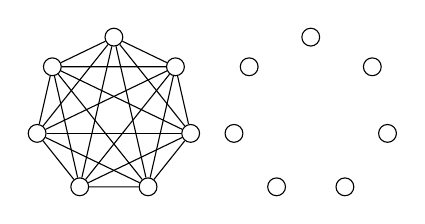
\begin{tikzpicture}
                \foreach \x in {0,...,6} {
                    \node [node] (\x) at (360/7*\x+90:1) {};
                    \node [node,xshift=2.5cm] (\x2) at (360/7*\x+90:1) {};
                }
                \foreach \x in {0,...,6} {
                    \foreach \y in {0,...,6} {
                        \ifnum \x<\y
                            \draw (\x) -- (\y);
                        \fi
                    }
                }
            \end{tikzpicture}
        \end{center}
\end{enumerate}

\subsubsection*{Simple upper bound}
List the vertices in some order, \hyperlink{def:colour}{colour} each in turn using the least colour not already used on its \hyperlink{def:neighbour}{neighbours}.
\hypertarget{def:greedy}This is often called a `\textbf{greedy algorithm}'.

When we colour $v$, there are at most $\hyperlink{def:degree}{d(v)} \leq \hyperlink{def:degree}{\Delta(G)}$ colours unavailable.
Thus
\begin{equation*}
    \chi(G) \leq \Delta(G) + 1 \tag{$*$} \label{eq:greedystar}
\end{equation*}
But e.g.\ if $G = \hyperlink{def:knn}{K_{1,t}}$ then $\hyperlink{def:chromNum}{\chi}(G)$ then $\chi(G) = 2$ but $\Delta(G) = t$.

For which graphs $G$ is \eqref{eq:greedystar} achieved?
\begin{itemize}
    \item $G$ complete: $\chi(\hyperlink{def:Kn}{K_k}) = k$, $\Delta(K_k) = k-1$.
    \item $G$ an odd \hyperlink{def:Cn}{cycle}, e.g.\ a pentagon: $\chi(G) = 3$, $\Delta(G) = 2$.
\end{itemize}

\begin{nthm}[Brooks' theorem]\label{thm:28}
    Let $G$ be a \hyperlink{def:components}{connected} graph that is neither \hyperlink{def:Kn}{complete} nor an odd \hyperlink{def:Cn}{cycle}.
    Then $\chi(G) \leq \Delta(G)$.
\end{nthm}
\begin{proof}
    Induction on \hyperlink{def:order}{$|G|$}. Write $\Delta = \hyperlink{def:degree}{\Delta}(G)$.
    We cannot have $\Delta = 0,1$ as $G \ncong \hyperlink{def:Kn}{K_1}, K_2$.
    If $\Delta = 2$ then $G$ is a \hyperlink{def:Pn}{path} or an even \hyperlink{def:Cn}{cycle}, so $\hyperlink{def:chromNum}{\chi}(G) = 2$.
    So assume $\Delta \geq 3$. Pick $v \in G$ and let $H$ be a \hyperlink{def:components}{component} of $G - v$.

    \textbf{Either} $\Delta(H) < \Delta$, in which case by greedy algorithm bound \eqref{eq:greedystar} we have \begin{equation*}\chi(H) \leq \Delta(H) + 1 \leq \Delta.\end{equation*}
    \textbf{Or} $\Delta(H) = \Delta$. Then $H$ is connected and not an odd cycle (as $\Delta \geq 3$).
    Moreover, $\exists u \in H$ with $u \hyperlink{def:neighbour}{\sim} v$ in $G$.
    In $G$, $d(u) \leq \Delta$ so in $H$, $d(u) \leq \Delta - 1$.
    So $H$ is not \hyperlink{def:regular}{regular}, so not complete.
    Hence by induction hypothesis, $\chi(H) \leq \Delta$.

    Do this for each component of $G - v$ to obtain a $\Delta$-\hyperlink{def:colour}{colouring} $c$ of $G - v$.
    If there is a colour missing from $\hyperlink{def:neighbour}{\Gamma}(v)$, then use that colour at $v$, as required.
    So assume that is not the case.

    So have $\Gamma(v) = \{x_1, \dotsc, x_\Delta\}$ with $\forall i, c(x_i) = i$.
    We can also assume:
    \begin{enumerate}[label=(\roman*)]
        \item if $i \neq j$ then there is an \hyperlink{def:ijpath}{$ij$-path} $P_{ij}$ from $x_i$ to $x_j$,
        \item if $i \neq j$ then $P_{ij}$ is entire \hyperlink{def:ijcomp}{$ij$-component} containing $x_i,x_j$, and
        \item if $i, j, k$ distinct then $P_{ij}, P_{ik}$ meet only at $x_i$.
    \end{enumerate}
    (Why? If any of these fail then it is easy to check that the colouring $c$ can be modified to change the colour of $x_i$ and allowing us to use colour $i$ at $v$).
    \begin{enumerate}[label=(\roman*)]
        \item is as in previous proofs.
        \item if $P_{\red{i}\green{j}}$ is not the entire $\red{i}\green{j}$-component, then
            at some point in the path we get a point (wlog colour \green{$j$}) which `branches off'.
            \begin{center}
                \begin{tikzpicture}
                    \node [node,       thick] (v) at (0,0) {};
                    \node [node,bgreen,thick] (j) at (0.2,1) {};
                    \node [node,bred,  thick] (i) at (1,-0.2) {};
                    \draw[path fading=west] (v) -- ( 170:1);
                    \draw[path fading=west] (v) -- (-160:1);
                    \draw[path fading=west] (v) -- (-140:1);
                    \draw[path fading=west] (v) -- (-130:1);
                    \draw[path fading=south] (v) -- ( -96:1);

                    \draw (j) -- (v) -- (i);
                    \node [node, bred,   thick] (i2) at (1.2,1.1) {};
                    \node [node, bgreen, thick] (j2) at (1.7,0.4) {};
                    \node [node, bgreen, thick] (j3) at (1.8,1.7) {};

                    \draw (j) -- (i2) -- (j3);
                    \draw (i2) -- (j2) -- (i);
                \end{tikzpicture}
            \end{center}
            Then this vertex has 3 \green{green} neighbours, so there are at most $\Delta - 3$ colours used in the rest of its neighbours, so there is a colour not in the colours of its neighbours$\cup \{i,j\}$.
            We can swap it to that, breaking the chain $P_{ij}$.
        \item if $P_{ij}, P_{ik}$ meet at some point which must have colour $i$, then that point has 2 $j$ neighbours and 2 $k$ neighbours, so as before there is a colour other than $i$ that none of its neighbours have, which we can swap it to, breaking $P_{ij}$ and $P_{ik}$.
    \end{enumerate}

    As $G \ncong K_{\Delta+1}$, there are some $i, j$ with $i \neq j$, $x_i \nsim x_j$.
    As $\Delta \geq 3$, pick $k \in [\Delta] \setminus \{i, j\}$.
    Let $u$ be the neighbour of $x_i$ of colour $j$.
    Swap colours $i,k$ on the $ik$-component of $x_i$ (i.e.\ on $P_{ik}$).
    This gives a new colouring $c'$, with $c'(x_i) = k$, $c'(x_k) = i$.

    Also, if $w \in P_{ij}$ with $w \neq x_i$ then $c'(w) = c(w)$ so $c'(x_j)=c'(u) = j$.
    $c'$ must satisfy conditions (i),(ii),(iii) as before.
    Then by (i) there is a $kj$-path from $x_i$ to $x_j$ , $P'_{kj}$ .
    By (ii), $u \in P'_{kj}$.

    By (i), there is a $ji$-path $P'_{ji}$ from $x_j$ to $x_k$.
    By (ii), $u \in P'_{ji}$.
    But now $P'_{kj}$ and $P'_{ji}$ meet at $u$, contradicting (iii).
\end{proof}

\subsection{Graphs on surfaces}
We've seen if $G$ can be \hyperlink{def:drawing}{drawn} in the plane then $\hyperlink{def:chromNum}{\chi(G)} \leq 4$.
What about other surfaces?

On the sphere, it is just the same.
But, we can draw \hyperlink{def:Kn}{$K_5$} on the torus (missing picture), and $\hyperlink{def:chromNum}{\chi}(K_5) = 5$.

There is a classification theorem for surfaces.
The closed surfaces without boundary are:
\begin{itemize}
    \item For $g \geq 0$, the \textbf{orientable surface of genus} $g$, the torus with $g$ holes called $T_g$.
    \item For $g \geq 1$, the \textbf{non-orientable surface of genus} $g$, the sphere with $g$ discs cut out and $g$ M\"obius strips sewn in called $S_g$.
\end{itemize}
\begin{eg}\leavevmode
    \begin{itemize}
        \item $T_0$ is the sphere, $T_1$ is the torus
        \item $T_3$ is shown here
            \begin{center}
                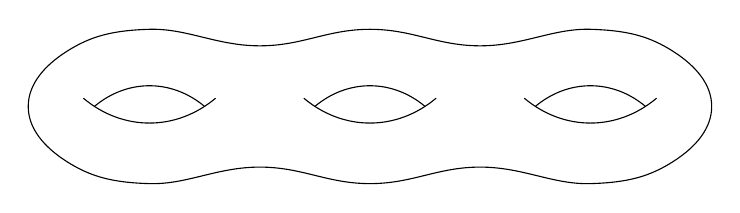
\begin{tikzpicture}[scale=0.7]
                    \draw (-1,0) to[bend left=40] (1,0);
                    \draw (-1.2,0.15) to[bend right=40] (1.2,0.15);
                    \draw ( 3,0) to[bend left=40] (5,0);
                    \draw ( 2.8,0.15) to[bend right=40] (5.2,0.15);
                    \draw ( 7,0) to[bend left=40] (9,0);
                    \draw ( 6.8,0.15) to[bend right=40] (9.2,0.15);
                    \draw plot [smooth cycle, tension=0.7] coordinates {
                            (-2.2, 0  )
                            (-1.5, 1  )
                            ( 0  , 1.4)
                            ( 2  , 1.1)
                            ( 4  , 1.4)
                            ( 6  , 1.1)
                            ( 8  , 1.4)
                            ( 9.5, 1  )
                            ( 10.2 , 0  )
                            ( 9.5,-1  )
                            ( 8  ,-1.4)
                            ( 6  ,-1.1)
                            ( 4  ,-1.4)
                            ( 2  ,-1.1)
                            ( 0  ,-1.4)
                            (-1.5,-1  )
                        };
                \end{tikzpicture}
            \end{center}
        \item $S_1$ is the real projective plane
        \item $S_2$ is the Klein bottle
    \end{itemize}
\end{eg}

\begin{defi}[Chromatic number of surface]\hypertarget{def:chromSur}
    Given a surface $S$, the \textbf{chromatic number of $S$} is
    \begin{equation*}
        \chi(S) = \max\set{\hyperlink{def:chromNum}{\chi}(G) | G \text{ can be \hyperlink{def:drawing}{drawn} on } S}
    \end{equation*}
\end{defi}
The \nameref{thm:27} says that $\hyperlink{def:chromSur}{\chi}(T_0) = 4$. Also $\chi(T_1) = 5$.
We use the \textbf{Euler-Poincar\'e Formula}: If $G$ can be drawn on $S$ with $l$ \hyperlink{def:face}{faces}, $\hyperlink{def:order}{\abs{G}} = n$, $\hyperlink{def:eG}{e(G)} = m$ then $n - m + l \geq E$, where $E$ is the \hypertarget{def:eulerChar}Euler characteristic of the surface given by
\begin{align*}
    S = T_g &\implies E = 2 - 2g \\
    S = S_g &\implies E = 2 - g
\end{align*}
\begin{nthm}[Heawood's Theorem]\label{thm:29}
    Let $S$ be a closed boundaryless surface of \hyperlink{def:eulerChar}{Euler characteristic} $E \leq 1$. Then
    \begin{equation*}
        \hyperlink{def:chromSur}{\chi(S)} \leq \floor*{\frac{7 + \sqrt{49-24E}}{2}}.
    \end{equation*}
\end{nthm}
\begin{proof}
    Let $\chi = \hyperlink{def:chromSur}{\chi(S)}$. Let $G$ be a minimal $\chi$-\hyperlink{def:colour}{colourable} graph that can be \hyperlink{def:drawing}{drawn} on $S$ - i.e.\ $\hyperlink{def:chromNum}{\chi}(G) = \chi$ but
    \begin{equation*}H \subset G, H \neq G \implies \chi(G) \leq \chi - 1.\end{equation*}
    Clearly $G$ is connected and $\hyperlink{def:order}{|G|} \geq \chi$.

    Let $|G| = n \geq \chi$, $\hyperlink{def:eG}{e(G)} = m$ and draw $G$ on $S$ with $l$ faces.
    Then by \hyperlink{def:eulerChar}{Euler-Poincar\'e}, $n - m + l \geq E$.
    As before, $l \leq \frac{2}{3} m$ so $n - \frac 13 m \geq E$ so $m \leq 3n - 3E$.
    Hence
    \begin{equation*}
        \hyperlink{def:degree}{\delta(G)} \leq \frac{2m}{n} \leq \frac{6n-6E}{n} = 6 - \frac{6E}{n}. \tag{$*$} \label{eq:heawoodstar}
    \end{equation*}
    On the other hand, if $v \in G$ then $G - v$ is $(\chi-1)$-colourable and this colouring does not extend to a $(\chi-1)$-colouring of $G$ so $d(v) \geq \chi-1$.
    Hence $\delta(G) \geq \chi-1$.

    Combining this with \eqref{eq:heawoodstar}:
    If $E \leq 0$: $\chi - 1 \leq \delta(G) \leq 6 - \frac{6E}{n} \leq 6 - \frac{6E}{\chi}$ as $n \geq \chi$.
    Hence $\chi^2 - 7\chi + 6E \leq 0$ and so $\chi \leq \frac{7 + \sqrt{49 + 24 E}}{2}$.

    If $E = 1$, $\delta(G) \leq 6 - \frac{6}{n} < 6$ so $\delta(G) \leq 5$. Hence $\chi-1 = 5$ so $\chi \leq 6 = \frac{7 + \sqrt{49 + 24}}{2}$.
\end{proof}
\begin{remark}
    The condition $E \leq 1$ takes out only the sphere.
    The theorem is true for the sphere (\nameref{thm:27}), but this proof doesn't work if $E = 2$.
\end{remark}

\begin{eg}
    Suppose $E = 0$, so $\hyperlink{def:chromSur}{\chi}(S) \leq 7$. There are 2 possible surfaces:
    \begin{enumerate}[label=(\roman*)]
        \item The torus $T_1$. We've seen \hyperlink{def:Kn}{$K_5$} can be \hyperlink{def:drawing}{drawn} on the torus.
            In fact, a $K_7$ can also be drawn on the torus, and so $\hyperlink{def:chromSur}{\chi}(T_1) = 7$.
        \item The Klein bottle $S_2$. It turns out $K_6$ can be drawn on the Klein bottle, but not $K_7$.
            So $6 \leq \chi(S_2) \leq 7$.
    \end{enumerate}
\end{eg}
Can we find $G$ on Klein bottle with $\hyperlink{def:chromNum}{\chi}(G) = 7$?
Suppose we can. Let $G$ be a minimal $7$-\hyperlink{def:chromNum}{chromatic} graph on $S_2$.

Examine the proof of \nameref{thm:29}. First, $G$ is \hyperlink{def:components}{connected}. Also $\hyperlink{def:degree}{\delta(G)} \geq 6$.
Then $6 \leq \delta(G) \leq \frac{2m}{n} \leq 6$.
So equality holds throughout. Thus $\delta(G) = 6$ and \hyperlink{def:degree}{average degree} 6, so $G$ is \hyperlink{def:regular}{6-regular}.
In particular, $G$ is connected, $\Delta(G) = 6$ and $\chi(G) = 7$. By \nameref{thm:28}, $G \cong K_7$, a contradiction.
So, $\chi(S_2) = 6.$

In fact the bound from \nameref{thm:29} is tight for all surfaces except the Klein bottle.
That is if $S \neq S_2$,
\begin{equation*}
    \hyperlink{def:chromSur}{\chi(S)} \leq \floor*{\frac{7 + \sqrt{49-24E}}{2}} = \chi.
\end{equation*}
Why? It turns out that $K_\chi$ can be drawn on $S$ (hard).

\subsection{Edge Colouring}
\begin{defi}[Edge colouring]\hypertarget{def:eColour}
    A $k$-edge colouring of a \hyperlink{def:graph}{graph} $G = (V,E)$ is a function $\varphi: E \to [k]$ such that if $e,e' \in E$ with precisely one common vertex then $\varphi(e) \neq \varphi(e')$.
\end{defi}
\begin{defi}[Edge chromatic number]\hypertarget{def:eChromNum}
    The \textbf{edge-chromatic number} of $G$ is
    \begin{equation*}
        \chi'(G) = \min \set{k | G \text{ has a $k$-\hyperlink{def:eColour}{edge colouring}}}.
    \end{equation*}
\end{defi}
Clearly $\hyperlink{def:degree}{\Delta(G)} \leq \hyperlink{def:eChromNum}{\chi'}(G) \leq 2 \Delta(G) - 1$, where the lower bound comes from a greedy algorithm: the worst case looks like
\begin{center}
    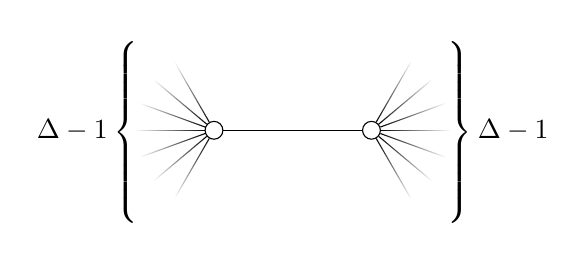
\begin{tikzpicture}
        \node [node] (A) at (0,0) {};
        \node [node] (B) at (2,0) {};
        \draw (A) -- (B);
        \foreach \x in {-3,...,3} {
            \draw [path fading=west] (A) -- +(\x*20 + 180:1);
            \draw [path fading=east] (B) -- +(\x*20:1);
        }
        \node at (-1.8,0) {$\Delta-1$};
        \node at (-1.1,0) {$\left\{\rule{0cm}{1.3cm}\right.$};
        \node at ( 3.1,0) {$\left.\rule{0cm}{1.3cm}\right\}$};
        \node at ( 3.8,0) {$\Delta-1$};
    \end{tikzpicture}
\end{center}
where we need to colour the central edge.
In fact, we can tighten the upper bound:
\begin{nthm}[Vizing's theorem]\label{thm:30}
    Let $G$ be a \hyperlink{def:graph}{graph}. Then
    \begin{equation*}
        \hyperlink{def:eChromNum}{\chi'}(G) \leq \hyperlink{def:degree}{\Delta(G)} + 1
    \end{equation*}
\end{nthm}
\begin{proof}
    Induction on $\hyperlink{def:eG}{e(G)}$. The $e(G) = 0$ case is immediate.

    For $e(G) > 0$, let $\Delta = \hyperlink{def:degree}{\Delta(G)}$. Pick an edge $xy$.
    By the induction hypothesis we can find an $(\Delta+1)$-\hyperlink{def:eColour}{edge colouring} of $G - x y_1$, call it $\varphi$.

    As $\Delta(G) < \Delta + 1$, there some colour `missing' at each vertex.
    Let $c_1$ be missing at $y_1$. If $c_1$ is also missing at $x$, then colour $xy_1$ with colour $c$, so done.

    If not, let $y_2 \in \hyperlink{def:neighbour}{\Gamma(x)}$ with $\varphi(x y_2) = c_1$ and let $c_2$ be missing at $y_2$.
    % possible pic missing
    Continue inductively ($*$):
    Given distinct $y_1, \dotsc, y_n \in \Gamma(x)$, distinct colours $c_1, \dotsc, c_k$ such that $c_i$ is missing at $y_i$ (for $1 \leq i \leq k$) and $\varphi(x y_{i+1}) = c_i$ (for $1 \leq i \leq k-1$).
    If $c_k$ is missing at $x$, re-colour $xy_i$ in colour $c_i$.
    Otherwise, let $y_{k+1} \in \Gamma(x)$ with $\varphi(x y_{k+1}) = c_k$.
    Let $c_{k+1}$ be missing at $y_k$. If $c_{k+1} \notin \{c_1, \dotsc, c_k\}$, continue as at ($*$).

    Otherwise assume WLOG $c_{k+1} = c_1$. (If instead $c_{k+1} = c_j$ for some $j > 1$, then uncolour $xy_j$, recolour $x y_i$ in colour $c_i$ for $1 \leq i < j$ and relabel $y_j, y_{j+1}, \dotsc$ as $y_1, y_2, \dotsc$).
    Let $c$ be a colour missing at $x$.
    Consider the $cc_1$ subgraph of $G$, i.e.\ only edges coloured $c$ or $c_1$.
    This subgraph has maximum degree $\leq 2$ so each component is a path or a cycle.
    Moreover, $x,y_1,y_{k+1}$ have degree $\leq 1$ in this subgraph so $x_1, y_1, y_{k+1}$ are not all in the same component.

    If $x,y_1$ in different $c c_1$ component, then swap $c,c_1$ on the component of $y_1$ and give $x y_1$ colour $c$.
    Otherwise $x, y_{k+1}$ in different components. In this case, uncolour $x y_{k+1}$ and recolour $x y_i$ with colour $c_i$ for $1 \leq i \leq k$.
    Then swap colours $c,c_1$ on the $c c_1$-component of $y_{k+1}$ and give $x y_{k+1}$ colour $c$.
\end{proof}

\clearpage
\section{Connectivity}
\subsection{The Marriage Problem}
\textbf{Legal note}: This problem was first posed in 1935. Note $1935 < 2014$, so marriage has 1 man and 1 woman.

Suppose we have $n$ women and $n$ men. For each woman, we have a list of `suitable' husbands. Can we marry everyone off?
Reformulate this as a \hyperlink{def:bipartite}{bipartite graph}: $X$ is the set of women, $Y$ is the set of men, and an edge denotes suitability.
\begin{defi}[Matching]\hypertarget{def:matching}
    Let $G$ be a \hyperlink{def:bipartite}{bipartite} graph with bipartition $(X,Y)$.
    A \textbf{matching} from $X$ to $Y$ is a set $M \subset E(G)$ such that $\forall x \in X$, $\exists$ unique $e \in M$ with $x \in e$ and for all $y \in Y$ there is at most one $e \in M$ with $y \in e$.
\end{defi}

When can we find a \hyperlink{def:matching}{matching}?
Obviously need $\forall x \in X$, $|\hyperlink{def:neighbour}{\Gamma(x)}| \geq 1$.
Also need if $x,y \in X$ distinct then $|\Gamma(x) \cup \Gamma(y)| \geq 2$.
In general, if $A \subset X$ then we need
\begin{equation*}
    \hypertarget{def:gam}|\Gamma(A)| \coloneqq \left|\bigcup_{x \in A} \Gamma(x)\right| \geq |A|.
\end{equation*}
Surprisingly, this is enough.
\begin{nthm}[Hall's Marriage Theorem]\label{thm:31}
    Let $G$ be a \hyperlink{def:bipartite}{bipartite} graph with bipartition $(X,Y)$.
    Then $G$ has a \hyperlink{def:matching}{matching} from $X$ to $Y$ iff $G$ satisfies \textbf{Hall's condition}:
    \begin{equation*}
        \hypertarget{def:hall}\forall A \subset X, \abs{\Gamma(A)} \geq |A|
    \end{equation*}
\end{nthm}
\begin{proof}
    $(\Rightarrow)$ is obvious. For $(\Leftarrow)$, use induction on $\hyperlink{def:order}{|X|}$.
    $|X|=0,1$ are immediate.

    For $|X|\geq 2$, there are two cases. The easy case has $|\hyperlink{def:gam}{\Gamma(A)}| > |A|$ for all $A \subset X$ with $A \neq \emptyset,X$.
    Pick any $x \in X$. $|\hyperlink{def:neighbour}{\Gamma(x)}| \geq 1$ so pick $y \in \Gamma(x)$.
    Look at $G - \{x,y\}$; this graph satisfies \hyperlink{def:hall}{Hall's condition}, so has a \hyperlink{def:matching}{matching} from $X - \{x\}$ to $Y - \{y\}$. Add edge $xy$, and done.

    The harder case has $|\Gamma(A)| = |A|$ for some $A \neq 0,X$.
    Let
    \begin{align*}
        G_1 &= \hyperlink{def:indSubgraph}{G[A \cup \Gamma(A)]} \\
        G_2 &= G[(X \setminus A) \cup (Y \setminus \Gamma(A))].
    \end{align*}
    \begin{center}
        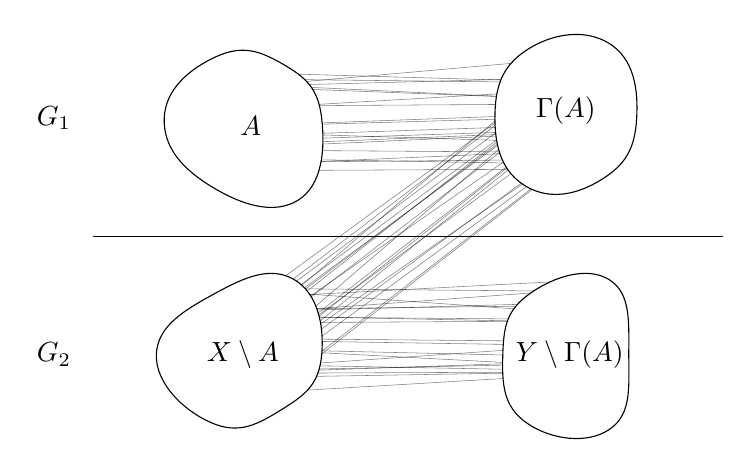
\begin{tikzpicture}
            \foreach \x in {1,...,20} {
                \draw[very thin,opacity=0.5] (0,2.25+\x/15+rand*0.2) -- (4,2.25+\x/15+rand*0.2);
                \draw[very thin,opacity=0.5] (0,-0.7+\x/15+rand*0.2) -- (4,2.4+\x/15+rand*0.2);
                \draw[very thin,opacity=0.5] (0,-0.5+\x/15+rand*0.2) -- (4,-0.5+\x/15+rand*0.2);
            }
            \draw[fill=white] plot [smooth cycle, tension=0.8]                       coordinates {(-180:1.2) (-120:1) (-60:0.8) (0:0.9) (60:1.1) (120:0.9)};
            \draw[fill=white] plot [smooth cycle, xshift=4cm, tension=0.8]           coordinates {(-180:0.8) (-120:1) (-60:1.1) (0:0.8) (60:1.1) (120:0.9)};
            \draw[fill=white] plot [smooth cycle, yshift=3cm, tension=0.8]           coordinates {(-180:1.1) (-120:1) (-60:1.2) (0:0.9) (60:0.8) (120:0.9)};
            \draw[fill=white] plot [smooth cycle, xshift=4cm,yshift=3cm,tension=0.8] coordinates {(-180:0.9) (-120:1) (-60:0.9) (0:0.9) (60:1.1) (120:1.0)};
            \node at (-2.5,3) {$G_1$};
            \node at (-2.5,0) {$G_2$};
            \node at (-0.1,0) {$X\setminus A$};
            \node at (0,2.9) {$A$};
            \node at (4,3.1) {$\Gamma(A)$};
            \node at (4.05,0) {$Y\setminus\Gamma(A)$};
            \draw (-2,1.5) -- (6,1.5);
        \end{tikzpicture}
    \end{center}
    First, $G_1$ obviously satisfies \hyperlink{def:hall}{Hall's condition} so $\exists$ a matching $A$ to $\Gamma(A)$.
    What about $G_2$? Take $B \subset X \setminus A$.
    Then
    \begin{equation*}|\Gamma_{G_2}(B)| = |\Gamma(A\cup B)\setminus \Gamma(A)| = |\Gamma(A \cup B)| - |\Gamma(A)| \geq |A \cup B| - |A|=|B|.\end{equation*}
    Hence $G_2$ also satisfies Hall and has a matching from $X \setminus A$ to $Y \setminus \Gamma(A)$.
    Combine the two matchings to get a matching from $X$ to $Y$ in $G$.
\end{proof}
\begin{defi}[Independent set]\hypertarget{def:indepEdg}
    Let $G = (V,E)$ be a \hyperlink{def:graph}{graph}.
    A set $F \subset E$ is \textbf{independent} if no two edges of $F$ share a vertex.
\end{defi}
Note: A matching from $X$ to $Y$ is just a set of $|X|$ \hyperlink{def:indepEdg}{independent} edges.
\begin{ncor}[Defect Hall]\label{cor:32}
    Let $G$ be a \hyperlink{def:bipartite}{bipartite} graph with bipartition $(X,Y)$ and let $d \geq 1$.
    Then $G$ contains $|X|-d$ independent edges if and only if $\forall A \subset X, \ |\Gamma(A)| \geq |A| - d$.
\end{ncor}
\begin{proof}
    ($\Rightarrow$) is immediate.
    ($\Leftarrow$). In marriage terminology: Introduce $d$ imaginary perfect men, suitable husbands for all the women.
    This satisfies \hyperlink{def:hall}{Hall's condition} so has matching from $X$ to $Y$.
    In real life, at most $d$ women unmarried.
\end{proof}
\begin{ncor}[Polyandrous Hall]\label{cor:33}
    Let $G$ be a \hyperlink{def:bipartite}{bipartite} graph, bipartition $(X,Y)$, $d \geq 2$.
    Then $G$ contains a set of $d |X|$ edges, each vertex in $X$ in precisely $d$ of them, each vertex in $Y$ in at most one $\iff \forall A \subset X, |\Gamma(A)| \geq d |A|$.
\end{ncor}
\begin{proof}
    ($\Rightarrow$) is immediate.
    ($\Leftarrow$). In marriage terminology: clone each woman $d-1$ times so there are $d$ copies of each.
    This satisfies \hyperlink{def:hall}{Hall's condition} so have matching from $X$ to $Y$.
    Destroy the clones.
\end{proof}
Further extensions are possible, e.g.\
\begin{enumerate}[label=(\roman*)]
    \item (Variable polyandrous) Take women $x_1, \dotsc, x_n$ and numbers $d_1, \dotsc, d_n \geq 1$. Give woman $x_i$ $d_i$ husbands.
    \item (Defect polyandrous) Aim to each each woman $d$ husbands but allow $d'$ `missing' husbands.
    \item (Same sex) (Harder) If $G$ is a \hyperlink{def:graph}{graph}, when can we find a 1-factor in $G$: a set of $\frac{\hyperlink{def:order}{|G|}}{2}$ independent edges.
\end{enumerate}

\subsection{Connectivity}
\begin{defi}[$k$-connectivity]\hypertarget{def:kConn}
    Let $k \geq 1$.
    We say a \hyperlink{def:graph}{graph} $G$ is \textbf{$k$-connected} if whenever $W \subset \hyperlink{def:order}{V(G)}$ with $\hyperlink{def:order}{|W|} < k$ then $G-W$ is \hyperlink{def:components}{connected}.
\end{defi}
(Assume for now that $G$ is not a complete graph).
\begin{eg}
    $G$ is \hyperlink{def:kConn}{1-connected} $\iff$ $G$ is \hyperlink{def:components}{connected}.
    $G$ is 2-connected $\iff G$ is connected and $G$ has no `cut vertex'.
        \begin{center}
            \begin{tikzpicture}
                \node [node] (A) at ( 0, 0) {};
                \node [node] (B) at ( 1, 1) {};
                \node [node] (C) at ( 1,-1) {};
                \node [thick,bred,node] (D) at ( 2, 0) {};
                \node [node] (E) at ( 3, 1) {};
                \node [node] (F) at ( 3,-1) {};
                \draw (A) -- (B) -- (D) -- (E) -- (F) -- (D) -- (C) -- (A);
            \end{tikzpicture}
        \end{center}
        The highlighted vertex is a cut vertex, and the graph is not 2-connected.
\end{eg}
\begin{defi}[Independent paths]\hypertarget{def:indepPath}
    Let $G$ be a graph and $a,b \in V$ be distinct.
    A collection of \hyperlink{def:path}{paths} from $a$ to $b$ is \textbf{independent} if the paths meet only at $a$ and $b$.
\end{defi}
Suppose for all distinct $a,b \in G$ there are $k$ \hyperlink{def:indepPath}{independent paths} from $a$ to $b$.
Then if $W \subset \hyperlink{def:order}{V(G)}$, $\hyperlink{def:order}{|W|} < k$ then $G - W$ is still \hyperlink{def:components}{connected}.
So $G$ is \hyperlink{def:kConn}{$k$-connected}.

What about a converse? If $G$ is \hyperlink{def:kConn}{$k$-connected} and we can only find $k-1$ \hyperlink{def:indepPath}{independent $ab$-paths} for some $a,b \in G$ then we would like to say `delete' one vertex from each path to disconnect the graph, reaching a contradiction.
But this is false, e.g.\
\begin{center}
    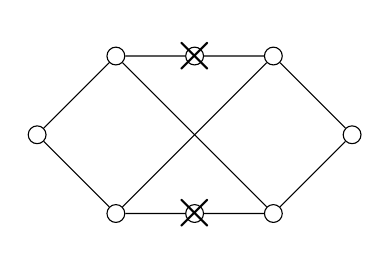
\begin{tikzpicture}
        \node [node] (A) at (-2, 0) {};
        \node [node] (B) at (-1, 1) {};
        \node [node] (C) at ( 0, 1) {};
        \node [node] (D) at ( 1, 1) {};
        \node [node] (E) at ( 2, 0) {};
        \node [node] (F) at ( 1,-1) {};
        \node [node] (G) at ( 0,-1) {};
        \node [node] (H) at (-1,-1) {};
        \draw (A) -- (B) -- (C) -- (D) -- (E) -- (F) -- (G) -- (H) -- (A);
        \draw (B) -- (F);
        \draw (D) -- (H);
        \node at (C) {\huge$\times$};
        \node at (G) {\huge$\times$};
    \end{tikzpicture}
\end{center}

In fact, the converse is true, but not obvious.
\begin{defi}[$AB$-path]\hypertarget{def:abpath}
    Let $G$ be a \hyperlink{def:graph}{graph} and $A,B \subset \hyperlink{def:order}{V(G)}$.
    An \textbf{$AB$-path} is a \hyperlink{def:path}{path} that meets $A$ in its first vertex and nowhere else, and meets $B$ in its last vertex and nowhere else.
    A set $W \subset V(G)$ is an $AB$-separator if $G-W$ contains no $AB$-path.
\end{defi}
\begin{remark}\leavevmode
    \begin{itemize}
        \item $A$ is an \hyperlink{def:abpath}{$AB$-separator}. Also, $B$ is an $AB$-separator.
        \item Suppose $G$ is \hyperlink{def:kConn}{$k$-connected}.
            Then as long as $|A|,|B| \geq k$ we have that any $AB$-separator $W$ satisfies $|W| \geq k$.
        \item Note that we do not suppose $A \cap B = \emptyset$.
            If $v \in A \cap B$ then $v$ is an \hyperlink{def:abpath}{$AB$-path} (of length zero).
            Thus for any $AB$-separator $W$, $A \cap B \subset W$.
    \end{itemize}
\end{remark}

\begin{nthm}\label{thm:34}
    Let $G$ be a \hyperlink{def:graph}{graph} and $A,B \subset \hyperlink{def:order}{V(G)}$.
    Let
    \begin{equation*}
        k = \min \set{\abs{W} | W \text{ is an \hyperlink{def:abpath}{$AB$-separator}}}.
    \end{equation*}
    Then $G$ contains $k$ vertex-disjoint \hyperlink{def:abpath}{$AB$-paths}.
\end{nthm}
\hypertarget{def:vertexDisjoint}Note \textbf{vertex-disjoint} means the paths don't even meet inside $A$ or $B$.
\begin{proof}
    Coming soon.
\end{proof}
\begin{ncor}[Menger's Theorem]\label{cor:35}
    Let $G$ be an \hyperlink{def:Kn}{incomplete} \hyperlink{def:kConn}{$k$-connected} graph and let $a,b \in V(G)$, $a \neq b$.
    Then $G$ contains \hyperlink{def:indepPath}{$k$ independent} $ab$-paths.
\end{ncor}
\begin{proof}
    Suppose first $a \hyperlink{def:neighbour}{\nsim} b$. Let $A = \hyperlink{def:neighbour}{\Gamma(a)}$ and $B = \Gamma(b)$.
    We have $G$ \hyperlink{def:kConn}{$k$-connected} and $G-A,G-B$ disconnected, so $\hyperlink{def:order}{|A|},|B|\geq k$.

    Hence, any \hyperlink{def:abpath}{$AB$-separator} $W$ has $|W| \geq k$, so by \Cref{thm:34}, there are $k$ \hyperlink{def:vertexDisjoint}{vertex-disjoint} $AB$ paths.
    Extend these to $a$,$b$.

    If instead $a \sim b$: $G-ab$ is $(k-1)$-connected, so has $k-1$ \hyperlink{def:indepPath}{independent} $ab$ paths by first part.
    $ab$ is another, as required.
\end{proof}
\begin{defi}[Connectivity]\hypertarget{def:connectivity}
    If $G$ is an incomplete graph, the \textbf{connectivity} of $G$ is
    \begin{equation*}
        \kappa(G) \coloneqq \max \left(\set{k \geq 1 | G \text{ is \hyperlink{def:kConn}{$k$-connected}}} \cup \{0\}\right).
    \end{equation*}
\end{defi}
In light of \Cref{cor:35}, define $\kappa(K_n) = n-1$ for $n \geq 2$.

We now return to prove \Cref{thm:34}: that if every \hyperlink{def:abpath}{$AB$-separator} has \hyperlink{def:order}{order} $\geq k$ then there are $k$ \hyperlink{def:vertexDisjoint}{vertex-disjoint} \hyperlink{def:abpath}{$AB$-paths}.
\begin{proof}[Proof of \Cref{thm:34}]
    Induction on \hyperlink{def:eG}{$e(G)$}.
    If $e(G) = 0$, the smallest \hyperlink{def:abpath}{$AB$-separator} is $A \cap B$, and each vertex of $A \cap B$ gives an \hyperlink{def:abpath}{$AB$-path} (of length zero), so done.

    If $e(G) > 0$, pick $xy \in \hyperlink{def:order}{E(G)}$.
    Let $W$ be an $AB$-separator of minimum \hyperlink{def:order}{order} in $G - xy$.
    If $|W| \geq k$ then by the induction hypothesis there are $k$ \hyperlink{def:vertexDisjoint}{vertex-disjoint} $AB$-paths in $G-xy$ and so also in $G$.

    So assume $|W| < k$. Then $W \cup \{x\}$ is an $AB$-separator in $G$.
    Hence $|W \cup \{x\}| \geq k$ so $|W| \geq k-1$ so $|W| = k-1$.
    Write $W = \{w_1, w_2, \dotsc, w_{k-1}\}$. As $|W| < k$, $G-W$ contains an $AB$-path.
    This path must include the edge $xy$.
    Assume WLOG $x$ comes before $y$ in this path (if not, swap $x$ and $y$).

    Let $X = W \cup \{x\}$ and $Y = W \cup \{y\}$.
    Let $U$ be an \hyperlink{def:abpath}{$AX$-separator} in $G-xy$. Then $U$ is an $AB$-separator in $G$, so $|U| \geq k$.
    So by the induction hypothesis, we have $k$ \hyperlink{def:vertexDisjoint}{vertex-disjoint} $AX$-paths in $G-xy$, say $P_0, P_1, \dotsc, P_{k-1}$ ending at $x, w_1, \dotsc, w_{k-1}$ respectively.

    Similarly, there are $k$ vertex-disjoint $YB$ paths in $G-xy$, say $Q_0, Q_1, \dotsc, Q_{k-1}$ starting at $y, w_1, w_2, \dotsc, w_{k-1}$ respectively.

    Given \hyperlink{def:path}{path} $P=u_0 u_1 \dotsm u_l$ and $Q = v_0 v_1 \dotsm v_m$ meeting only at $u_l = v_0$, write $P \vee Q$ for the path $u_0 \dotsm u_l v_1 \dotsm v_m$.
    Then $P_0 \vee xy \vee Q_)$ and $P_i \vee Q_i$ (for $1 \leq i \leq k-1$) are $k$ vertex-disjoint $AB$-paths in $G$.
\end{proof}
In fact, \nameref{thm:31} is also a consequence of \Cref{thm:34}.
Let $G$ be a \hyperlink{def:bipartite}{bipartite} graph with bipartition $(X,Y)$ such that
\begin{equation*}
    \forall A \subset X, |\Gamma(A)| \geq |A|.
\end{equation*}
Let $W$ be an \hyperlink{def:abpath}{$XY$-separator}.
Then $\Gamma(X \setminus W) \subset Y \cap W$ so
\begin{align*}
    |W| &= |X \cap W| + |Y \cap W| \\
        &\geq |X \cap W| + |\Gamma(X \setminus W)| \\
        &\geq |X \cap W| + |X \setminus W| = |X|.
\end{align*}
Hence by \Cref{thm:34} we have $|X|$ \hyperlink{def:vertexDisjoint}{vertex-disjoint} \hyperlink{def:abpath}{$XY$-paths}, i.e.\ a \hyperlink{def:matching}{matching} from $X$ to $Y$.
\subsection{Edge connectivity}
\begin{defi}[$l$-edge connected]\hypertarget{def:lConn}
    Let $G$ be a \hyperlink{def:graph}{graph} with $|G| \geq 2$ and let $l \geq 1$.
    We say $G$ is \textbf{$l$-edge connected} if whenever $D \subset E(G)$ with $|D| < l$ we have $G-D$ connected.
    The \textbf{edge-connectivity} of $G$ is
    \begin{equation*}
        \lambda(G) \coloneqq \max \left(\set{l \geq 1 | G \text{ is \hyperlink{def:lConn}{$l$-edge connected}}} \cup \{0\}\right).
    \end{equation*}
\end{defi}
\begin{ncor}[Edge Menger]\label{cor:36}
    Let $G$ be \hyperlink{def:lConn}{$l$-edge connected} and $a,b \in V(G)$ be distinct.
    Then $G$ has $l$ edge-disjoint \hyperlink{def:abpath}{$ab$-paths}.
\end{ncor}
\begin{proof}
    The \hypertarget{def:linegraph}{\textbf{line graph}} of $G=(V,E)$ is the graph $L(G) = (E,F)$ where
    \begin{equation*}
        F = \set{ee' | e,e' \in E,\ e,e' \text{ share precisely one vertex}}.
    \end{equation*}
    Then $L(G)$ is \hyperlink{def:kConn}{$l$-connected}.
    Add extra vertices $a',b'$ to $L(G)$ with
    \begin{itemize}
        \item $a'$ joined to each $e \in E$ with $a \in e$ and
        \item $b'$ joined to each $e \in E$ with $b \in e$.
    \end{itemize}

    By \Cref{cor:35}, $L(G)$ has $l$ \hyperlink{def:indepPath}{independent} \hyperlink{def:abpath}{$a'b'$-paths}.
    This yields $l$ edge-disjoint $ab$-paths in $G$.
\end{proof}

\clearpage
\section{Probabilistic Techniques}
\subsection{The Probabilistic Method}
Recall the \hyperlink{def:ramseyNum}{Ramsey number} $R(s)$.
From \Cref{cor:3}, we have $R(s) = \hyperlink{def:asymp}{\mathcal{O}}(4^s)$.
What about lower bounds?
On example sheet 1, we get
\begin{itemize}
    \item $R(s) = \hyperlink{def:asymp}{\Omega}(s^2)$ (simple colouring)
    \item $R(s) = \Omega(s^3)$ (much harder).
\end{itemize}
A similar but much harder still method gives $R(s) = \Omega(s^4)$.
But this doesn't even give, say, $R(s) = \Omega(1.000001^s)$.
Remarkably,
\begin{nthm}[Erd\H{o}s]\label{thm:37}
    \begin{equation*}
        \hyperlink{def:ramseyNum}{R(s)} = \hyperlink{def:asymp}{\Omega}(\sqrt{2}^s)
    \end{equation*}
\end{nthm}
\begin{proof}
    Fix $n,s$. Colour each edge of $\hyperlink{def:Kn}{K_n}$ \red{red}/\green{green} at random, independently, each colour equally likely.
    Given $H \subset K_n$ with $H \cong K_s$,
    \begin{align*}
        \mathbb{P}(H\text{ monochromatic}) &= 2 \mathbb{P}(H\text{ \red{red}}) = 2 \times \left(\frac{1}{2}\right)^{\binom{s}{2}}. \\
        \shortintertext{So}
        \mathbb{P}(K_n \text{ has a monochromatic } K_5) &\leq \binom{n}{s} \cdot 2 \cdot \left(\frac{1}{2}\right)^{\binom{s}{2}}  \\
                                        &\leq \frac{n^s}{s!} \cdot 2 \left(\frac{1}{2}\right)^{\binom{s}{2}} \\
                                        &\leq n^s \cdot 2^{-\frac{s(s-1)}{2}} \\
                                        &= \left(\frac{n}{\sqrt{2}^{s-1}}\right)^s < 1 \quad \text{if $n < \sqrt{2}^{s-1}$.}
    \end{align*}
    So if $n < \sqrt{2}^{s-1}$ then there is \emph{some} colouring with no monochromatic $K_5$.
    So $R(s) \geq \sqrt{2}^{s-1}$.
\end{proof}

\subsection{Modifying a Random Graph}
In the proof of \Cref{thm:37}, we randomly coloured \hyperlink{def:Kn}{$K_n$} \red{red}/\green{green}, showed that
\begin{equation*}
    \mathbb{P}(\text{no mono }K_s) > 0
\end{equation*}
and deduced there must be a colouring with no monochromatic $K_s$.
In general, we do something random, show
\begin{equation*}
    \mathbb{P}(\text{thing we want happens}) > 0 \tag{$*$} \label{eq:5.2star}
\end{equation*}
and deduce that sometimes the thing we want happens.

Sometimes it is too hard to prove \eqref{eq:5.2star} directly and we have to work a bit harder.
Instead, show $\mathbb{P}(\text{thing we want `almost happens'}) > 0$.
Take an example where the thing `almost happens', and modify it somehow to get what we want.

Recall the \hyperlink{def:zara}{Problem of Zarankiewicz}.
\Cref{thm:12} gave an upper bound: if $t \geq 2$ then $\hyperlink{def:zara}{z(n,t)} = \hyperlink{def:asymp}{\mathcal{O}}(n^{2 - \frac{1}{t}})$. What about lower bounds?
\begin{nthm}\label{thm:38}
    If $t \geq 2$ then $\hyperlink{def:zara}{z(n,t)} = \hyperlink{def:asymp}{\Omega}(n^{2 - \frac{2}{t+1}})$.
\end{nthm}
\begin{proof}
    Strategy: Given $n,p$, let $G$ be a random \hyperlink{def:bipartite}{bipartite} graph with vertex classes $X,Y$ with $\hyperlink{def:order}{|X|}=|Y|=n$, where for each $x \in X$, $y \in Y$ we have $xy \in E(G)$ with probability $p$, independently.
    Let $A = \hyperlink{def:eG}{e(G)}$ and $B$ be the number of copies of $\hyperlink{def:knn}{K_{t,t}}$ in $G$ (so $A$,$B$ are random variables).

    Aim: Given $n$, try to choose $p$ such that $\mathbb{E}(A-B)$ is large, specifically $\mathbb{E}(A-B) = \Omega(n^{2 - \frac{2}{t+1}})$.
    Then we can find a specific graph $G$ with $A-B = \Omega(n^{2-\frac{2}{t+1}})$.
    Remove an edge from each $K_{t,t}$ in $G$ to form a graph $H$ with no $K_{t,t}$ and $e(H) = \Omega(n^{2 - \frac{2}{t+1}})$, as required.

    Now, $\mathbb{E}(A) = n^2 p$ and $\mathbb{E}(B) = \binom{n}{t}^2 p^{t^2} \leq \frac{1}{(t!)^2} n^{2t}p^{t^2}$.
    So $\mathbb{E}(A-B) \geq n^2 p - \frac{1}{t!^2} n^{2t} p^{t^2}$.

    We want $n^2 p = n^{2t} p^{t^2}$ i.e.\ $p = n^{\frac{2-2t}{t^2-1}} = n^{-\frac{2}{t+1}}$.
    So, take $p = n^{-\frac{2}{t+1}}$.
    Then
    \begin{equation*}
        \mathbb{E}(A-B) \geq \left(1 - \frac{1}{(t!)^2}\right) n^{2 - \frac{2}{t+1}}. \qedhere
    \end{equation*}
\end{proof}
Recall from Example sheet 2 that there is a \hyperlink{def:Kn}{$\triangle$}-free graph of large \hyperlink{def:chromNum}{chromatic number} (a hard result).
What if we also ban \hyperlink{def:cycle}{cycles} of length 4? This is much harder still. In fact:
\begin{nthm}\label{thm:39}
    Let $g \geq 3$, $k \geq 2$. Then there is a graph $G$ with no \hyperlink{def:cycle}{cycles} of length $\leq g$ and $\hyperlink{def:chromNum}{\chi(G)} \geq k$.
\end{nthm}
\begin{proof}
    Strategy: Fix $n$ and $p$. Let $G$ be a random graph with $n$ vertices, each possible edge present independently with probability $p$.
    Let $X$ be the number of short \hyperlink{def:cycle}{cycles} in $G$.
    Recall that $\hyperlink{def:chromNum}{\chi(G)} \geq \frac{|G|}{\alpha(G)}$ where \hyperlink{def:indepNum}{$\alpha(G)$ is the independence number} of $G$.
    For cycles, by `short', we mean of length $\leq g$.

    Aim: Pick $n$ and $p$ such that
    \begin{enumerate}
        \item $\mathbb{P}(X > \frac{n}{2}) < \frac{1}{2}$ and
        \item $\mathbb{P}(\alpha(G) \geq \frac{n}{2k}) > \frac{1}{2}$.
    \end{enumerate}
    Then $\mathbb{P}(X > \frac{n}{2} \text{ or } \alpha(G) \geq \frac{n}{2k}) < 1$ so can pick a specific $G$ such that $X \leq \frac{n}{2}$ and $\alpha(G) < \frac{n}{2k}$.
    Remove a vertex from each short cycle to get $H$ with $|H| \geq \frac{n}{2}$ and $\alpha(H) < \frac{n}{2k}$ so $\chi(H) > \frac{n/2}{n/(2k)} = k$, as required.

    \begin{enumerate}
        \item For $3 \leq i \leq g$, let $X_i$ be the number of cycles of length $i$ appearing as subgraphs of $G$.
            Then
            \begin{equation*}
                \mathbb{E}(X_i) = \binom{n}{i} \frac{i!}{2i} p^i \leq (np)^i.
            \end{equation*}
            Now $X = \sum_{i=3}^g X_i$ so
            \begin{equation*}
                \mathbb{E}(X) \leq \sum_{i=3}^g (np)^i < g (np)^g \text{ as long as } np \geq 1. \label{eq:5.2star2}\tag{$*$}
            \end{equation*}
            By Markov,
            \begin{equation*}
                \mathbb{P}\left(X > \frac{n}{2}\right) \leq \frac{\mathbb{E}(X)}{n/2} < 2g n^{g-1} p^g \leq \frac{1}{2}
            \end{equation*}
            if $p \leq (\frac{1}{4g})^{\frac{1}{g}} n^{\frac{1}{g}-1}$.
            Take $p = (\frac{1}{4g})^{\frac{1}{g}} n^{\frac{1}{g}-1}$.
            Then $np = \left(\frac{1}{4g}\right)^\frac{1}{g} n^{\frac{1}{g}} \geq 1$ if $n$ sufficiently large, satisfying the condition of \eqref{eq:5.2star2}.
        \item \begin{align*}
                \mathbb{P}\left(\alpha(G) \geq \frac{n}{2k}\right) &\leq \binom{n}{\frac{n}{2k}} (1-p)^{\binom{n/2k}{2}} \\
                                                        &\leq n^{\frac{n}{2k}} e^{-p\frac{n^2}{16k^2}} \\
                                                        &= \exp\left\{\frac{2}{2k} \log n - \frac{n^2}{16k^2} \left(\frac{1}{4g}\right)^{\frac{1}{g}} n^{\frac{1}{g}-1}\right\} \to 0 \text{ as } n \to \infty.
            \end{align*}
            So if $n$ is sufficiently large, $\mathbb{P}(\alpha(G) \geq \frac{n}{2k}) < \frac{1}{2}$. \qedhere
    \end{enumerate}
\end{proof}

\subsubsection*{Properties of Expectation}
We used:
\begin{enumerate}
    \item \hypertarget{def:linear}{\textbf{Linearity of expectation}}.
        \begin{equation*}
            \mathbb{E}\left(\sum_{i=1}^n X_i\right) = \sum_{i=1}^n \mathbb{E}(X_i).
        \end{equation*}
        For example, we had $G$ \hyperlink{def:bipartite}{bipartite}, $n$ vertices in each class and each possible edge present independently with probability $p$; $B$ the number of $\hyperlink{def:knn}{K_{t,t}}$s in $G$.
        We said
        \begin{equation*}
            \mathbb{E}B = \binom{n}{t}^2 p^{t^2}.
        \end{equation*}
        Why? Let $H_1, \dotsc, H_N$ be the possible $K_{t,t}$s, where $N = \binom{n}{t}^2$.
        Let
        \begin{equation*}
            X_i =
            \begin{cases*}
                1 & if $H_i$ appears in $G$ \\
                0 & if not
            \end{cases*}
        \end{equation*}
        so $\mathbb{E}X_i = \mathbb{P}(H_i \text{ appears}) = p^{t^2}.$
        Then $B = \sum_{i=1}^N X_i$ so
        \begin{equation*}
            \mathbb{E}B = \sum_{i=1}^N \mathbb{E}X_i = N \mathbb{E}X_1 = \binom{n}{t}^2 p^{t^2}
        \end{equation*}
        as desired.
    \item \hypertarget{def:markov}{\textbf{Markov's inequality}}.
        If $X$ is a nonnegative random variable with finite mean and $\lambda > 0$ then
        \begin{equation*}
            \mathbb{P}(X \geq \lambda) \leq \frac{\mathbb{E}X}{\lambda}.
        \end{equation*}
        Proof: $\lambda \mathbbm{1}_{X \geq \lambda} \leq X$. Take expectations, giving $\lambda \mathbb{P}(X \geq \lambda) \leq \mathbb{E} X$.
    \item \hypertarget{def:cheby}{\textbf{Chebyshev's inequality}}.
        Let $X$ be a random variable with finite mean $\mu$ and finite variance $\sigma^2$. Then
        \begin{equation*}
            \forall \epsilon > 0 \quad \mathbb{P}(|X - \mu| \geq \epsilon) \leq \frac{\sigma^2}{\epsilon^2}.
        \end{equation*}
        Proof: Apply \hyperlink{def:markov}{Markov's inequality} to the random variable $(X - \mu)^2$ with mean $\sigma^2$.
\end{enumerate}

\subsection{The Structure of Random Graphs}
\hypertarget{def:gnp}Given $n \geq 1$ and $p \in [0,1]$ the probability space $\mathcal{G}(n,p)$ consists of all \hyperlink{def:graph}{graphs} $G$ with vertex set $[n]=\{1,2,\dotsc,n\}$ where for $i,j \in [n]$ distinct, $\mathbb{P}(ij \in E(G)) = p$, independently for different edges.
What does a typical $G \in \hyperlink{def:gnp}{\mathcal{G}(n,p)}$ look like?

For example, does $G$ contain a \hyperlink{def:Kn}{$\triangle$}?
Yes usually if $p$ large, no usually if $p$ small.
We might expect a curve as on the left, but in fact it more closely resembles the right.
\begin{center}
    \begin{tikzpicture}
        \begin{scope}[scale=2]
            \draw [->] (-0.2,0) -- (1.2,0);
            \draw [->] (0,-0.2) -- (0,1.2);
            \draw [fill] (0,1) circle [radius=0.2mm];
            \draw [fill] (1,1) circle [radius=0.2mm];
            \draw [fill] (1,0) circle [radius=0.2mm];
            \draw (0,0) to[bend right] (1,1);
            \node at (1.3,0) {$p$};
            \node at (0,1.35) {$\mathbb{P}(\triangle)$};
            \node at (-0.1,1) {$1$};
            \node at (1,-0.15) {$1$};
        \end{scope}
        \begin{scope}[scale=2,xshift=3cm]
            \draw [->] (-0.2,0) -- (1.2,0);
            \draw [->] (0,-0.2) -- (0,1.2);
            \draw [fill] (0,1) circle [radius=0.2mm];
            \draw [fill] (1,1) circle [radius=0.2mm];
            \draw [fill] (1,0) circle [radius=0.2mm];
            \draw plot [smooth,tension=0.4] coordinates {(0,0) (0.4,0.1)  (0.6,0.9) (1,1)};
            \node at (1.3,0) {$p$};
            \node at (0,1.35) {$\mathbb{P}(\triangle)$};
            \node at (-0.1,1) {$1$};
            \node at (1,-0.15) {$1$};
        \end{scope}
    \end{tikzpicture}
\end{center}
That is, we get a `sharp threshold', so to say.

First, consider an easier example: Does $G$ contain an edge?
Let $G \in \hyperlink{def:gnp}{\mathcal{G}(n,p)}$ and let $X = \hyperlink{def:eG}{e(G)}$.
Let $\mu = \mathbb{E}X = \binom{n}{2}p = Np$, writing $N = \binom{n}{2}$.
By \hyperlink{def:markov}{Markov},
\begin{equation*}
    \mathbb{P}(G\text{ has an edge}) = \mathbb{P}(X \geq 1) \leq \mathbb{E}X = Np.
\end{equation*}
So if $\mu = Np \to 0$ as $n \to \infty$, then $\mathbb{P}(G\text{ has an edge}) \to 0$.
That is, if $p = \hyperlink{def:asymp}{o}(\frac{1}{N}) = o(n^{-2})$ then $\mathbb{P}(G\text{ has an edge}) \to 0$.

What if $p$ is bigger, say $p = \hyperlink{def:asymp}{\omega}(n^{-2})$?
Then $\mu = Np \to \infty$, and we need to think about variance.
What is $\Var(X)$?
Let $e_1, e_2, \dotsc, e_N$ be the possible edges of $G$ and let
\begin{equation*}
    X_i =
    \begin{cases*}
        1 & if $e_i$ appears in $G$ \\
        0 & if not
    \end{cases*}
\end{equation*}
then $X = \sum_{i=1}^N X_i$.
Now $\mathbb{E}X_i = p$ and $\mathbb{E}X_i^2 = p$ so $\Var(X_i) = p - p^2$.
The $X_i$s are independent so
\begin{equation*}\Var(X) = \sum_{i=1}^N \Var(X_i) = N(p-p^2) \eqqcolon \sigma^2.\end{equation*}
By \hyperlink{def:cheby}{Chebyshev},
\begin{align*}
    \mathbb{P}(X=0) &\leq \mathbb{P}(|X-\mu|\geq \mu) \leq \frac{\sigma^2}{\mu^2} \\
                    &=\frac{N(p-p^2)}{(Np)^2} = \frac{1}{Np} - \frac{1}{N} \\&= \frac{1}{\mu} - \frac{1}{N} \leq \frac{1}{\mu} \to 0 \text{ as } n \to \infty.
\end{align*}
since $\mu \to \infty$ as $n \to \infty$.
So if $p = \omega(n^{-2})$ then $\mathbb{P}(X = 0) \to 0$ so $\mathbb{P}(X\geq 1) \to 1$ i.e.\ $\mathbb{P}(G\text{ has an edge}) \to 1$.

\textbf{We have proved}: $p = n^{-2}$ is a `sharp threshold' for $G \in \hyperlink{def:gnp}{\mathcal{G}(n,p)}$ in the sense that
\begin{itemize}
    \item if $p = \hyperlink{def:asymp}{o}(n^{-2})$ then almost every $G \in \mathcal{G}(n,p)$ has no edge, whereas
    \item if $p = \hyperlink{def:asymp}{\omega}(n^{-2})$ then almost every $G \in \mathcal{G}(n,p)$ has an edge.
\end{itemize}
\hypertarget{def:ae}Here, we say `almost every $G \in \mathcal{G}(n,p)$ has property $Q$' to mean
\begin{equation*}
    \mathbb{P}(G \in \hyperlink{def:gnp}{\mathcal{G}(n,p)} \text{ has } Q) \to 1 \text{ as } n \to \infty.
\end{equation*}
(Note this is different from terminology usually used by probabilists.)

More generally, let $A_1, A_2, \dotsc, A_n$ be events, $X$ is the number of $A_i$ that occur.
Then $X = \sum_{i=1}^n X_i$ where
\begin{equation*}
    X_i =
    \begin{cases*}
        1 & if $A_i$ occurs \\
        0 & if not
    \end{cases*}
\end{equation*}
so $\mathbb{E}X_i = \mathbb{P}(A_i)$. Hence by \hyperlink{def:linear}{linearity of expectation},
\begin{equation*}
    \boxed{\mathbb{E}X = \sum_{i=1}^n \mathbb{P}(A_i)}
\end{equation*}
We know $\Var(X) = \mathbb{E}X^2 - (\mathbb{E}X)^2$. Now,
\begin{align*}
    \mathbb{E}X^2 &= \mathbb{E}\left[\left(\sum_{i=1}^n X_i\right)^2\right] =\mathbb{E}\left[\left(\sum_{i=1}^n X_i\right)\left(\sum_{j=1}^n X_j\right)\right] \\
                  &= \mathbb{E}\sum_{i=1}^n \sum_{j=1}^n X_i X_j = \sum_{i=1}^n \sum_{j=1}^n \mathbb{E}(X_iX_j) \\
                  &= \sum_{i=1}^n \sum_{j=1}^n \mathbb{P}(A_i \cap A_j).
    \shortintertext{and}
    (\mathbb{E}X)^2 &= \left(\sum_{i=1}^n \mathbb{P}(A_i)\right)^2 = \sum_{i=1}^n \sum_{j=1}^n \mathbb{P}(A_i) \mathbb{P}(A_j).
\end{align*}
Hence
\begin{equation*}
    \Var(X) = \sum_{i=1}^n \sum_{j=1}^n \left(\mathbb{P}(A_i \cap A_j) - \mathbb{P}(A_i)\mathbb{P}(A_j)\right)
\end{equation*}
Note: Supposing $A_i$ and $A_j$ are independent, $\mathbb{P}(A_i \cap A_j) - \mathbb{P}(A_i) \mathbb{P}(A_j) = 0$.
So independent pairs do not contribute to this sum.

\begin{nprop}\label{prop:40}
    $p = \frac{1}{n}$ is a sharp threshold for $G \in \hyperlink{def:gnp}{\mathcal{G}(n,p)}$ to contain a $\triangle$, in the sense that:
    \begin{itemize}
        \item if $p = \hyperlink{def:asymp}{o}(\frac{1}{n})$ then \hyperlink{def:ae}{almost every} $G \in \mathcal{G}(n,p)$ has no $\triangle$, whereas
        \item if $p = \hyperlink{def:asymp}{\omega}(\frac{1}{n})$ then almost every $G \in \mathcal{G}(n,p)$ has a $\triangle$.
    \end{itemize}
\end{nprop}
\begin{proof}
    Let $G \in \hyperlink{def:gnp}{\mathcal{G}(n,p)}$ and let $X$ be the number of $\triangle$s in $G$.
    Let $\mu = \mathbb{E}X$ and $\sigma^2 = \Var(X)$.
    Then $\mu = \binom{n}{3} p^3 \sim \frac{1}{6} (np)^3$.
    Also,
    \begin{equation*}
        \sigma^2 = \underset{
            \begin{tikzpicture}[scale=0.5,every node/.style={node,inner sep=0.5mm},yshift=-2cm]
                \node (1) at (90:1) {};
                \node (2) at (-30:1) {};
                \node (3) at (-150:1) {};
                \draw (1) -- (2) -- (3) -- (1);
            \end{tikzpicture}
        }{\binom{n}{3} (p^3 - p^6)}
        + \underset{
            \begin{tikzpicture}[scale=0.5,every node/.style={node,inner sep=0.5mm},yshift=-1.7cm]
                \node (1) at (90:1) {};
                \node (2) at (-90:1) {};
                \node (3) at (-180:1) {};
                \node (4) at (0:1) {};
                \draw (1) -- (2) -- (3) -- (1) -- (4) -- (2);
            \end{tikzpicture}
        }
        {\binom{n}{3} \cdot 3 \cdot (n-3) (p^5 - p^6)}
        \leq n^3 p^3 + n^4 p^5.
    \end{equation*}

    Suppose first $p = \hyperlink{def:asymp}{\mathcal{o}}(\frac{1}{n})$, i.e.\ $np \to 0$. Then by \hyperlink{def:markov}{Markov},
    \begin{equation*}
        \mathbb{P}(X = 0) = 1 - \mathbb{P}(X \geq 1) \geq 1 - \mu \to 1 \text{ as } n \to \infty.
    \end{equation*}

    Suppose instead $p = \hyperlink{def:asymp}{\omega}(\frac{1}{n})$ so $n p \to \infty$. Then with \hyperlink{def:cheby}{Chebyshev},
    \begin{equation*}
        \frac{\sigma^2}{\mu^2} \leq \frac{1}{\mu^2} (n^3 p^3 + n^4 p^5) \sim \frac{36}{n^6 p^6} (n^3 p^3 + n^4 p^5) = \frac{36}{(np)^3} + \frac{36}{n\cdot np} \to 0 \text{ as } n \to \infty. \qedhere
    \end{equation*}
\end{proof}

We next wonder: What is the \hyperlink{def:cliqueNum}{clique number} $\omega(G)$ for a typical $G \in \hyperlink{def:gnp}{\mathcal{G}(n,p)}$?
\begin{center}
    \begin{tikzpicture}
        \begin{scope}[scale=1.5]
            \draw [->] (-0.2,0) -- (2.2,0);
            \draw [->] (0,-0.2) -- (0,1.2);
            \draw plot [smooth,tension=1] coordinates {(0,0) (1,0.8) (2,0)};
            \node at (2.3,0) {$k$};
            \node at (0,1.35) {$\mathbb{P}(\hyperlink{def:cliqueNum}{\omega}(G) = k)$};
            \node at (2,-0.15) {$n$};
        \end{scope}
        \begin{scope}[scale=1.5,xshift=4cm]
            \draw [->] (-0.2,0) -- (2.2,0);
            \draw [->] (0,-0.2) -- (0,1.2);
            \draw plot [smooth,tension=0.4] coordinates {(0,0) (0.85,0.1) (1,0.9) (1.15,0.1) (2,0)};
            \node at (2.3,0) {$k$};
            \node at (0,1.35) {$\mathbb{P}(\omega(G) = k)$};
            \node at (2,-0.15) {$n$};
        \end{scope}
    \end{tikzpicture}
\end{center}
We might guess a picture on the left, but in fact it is closer to the right: we have a `sharp concentration', so to say.
\begin{nthm}\label{thm:41}
    There exists a function $d: \mathbb{N} \to \mathbb{N}$ such that \hyperlink{def:ae}{a.e.\ }$G \in \hyperlink{def:gnp}{\mathcal{G}(n,p)}$ has $\hyperlink{def:cliqueNum}{\omega}(G) \in \{d-1,d,d+1\}$ (where $d = d(n)$).
\end{nthm}
\begin{proof}[Proof sketch]
    \textbf{(Currently missing).}
\end{proof}
\begin{remark} \leavevmode
    \begin{enumerate}
        \item This also shows that \hyperlink{def:ae}{a.e.\ }$G$ in $\hyperlink{def:gnp}{\mathcal{G}(n,p)}$ has $\hyperlink{def:cliqueNum}{\omega}(G) \sim 2 \log_2 n = \frac{2 \log n}{\log 2}$.
        \item The same proof works to give a similar result for general $p$. Then $\omega(G) \sim \frac{2 \log n}{\log \frac{1}{p}}$.
    \end{enumerate}
\end{remark}
\begin{ncor}\label{cor:42}
    \hyperlink{def:ae}{Almost every} $G \in \hyperlink{def:gnp}{\mathcal{G}(n,p)}$ has
    \begin{equation*}
        \hyperlink{def:chromNum}{\chi}(G) \geq (1 + o(1))\frac{n \log \frac{1}{q}}{2 \log n}
    \end{equation*}
    where $q = 1-p.$
\end{ncor}
\begin{proof}
    Let $G \in \hyperlink{def:gnp}{\mathcal{G}(n,p)}$. Then $\hyperlink{def:complement}{\overline{G}} \in \mathcal{G}(n,q)$.
    So by \Cref{thm:41}, with probability tending to 1 as $n \to \infty$ we have
    \begin{align*}
        \hyperlink{def:cliqueNum}{\omega}(\overline{G}) &\sim \frac{2 \log n}{\log \frac{1}{q}} \\
        \implies \hyperlink{def:indepNum}{\alpha(G)} &\sim \frac{2 \log n}{\log \frac{1}{q}}\\
        \implies \hyperlink{def:chromNum}{\chi}(G) &\geq \frac{|G|}{\alpha(G)} \sim \frac{n \log \frac{1}{q}}{2 \log n}. \qedhere
    \end{align*}
\end{proof}

In fact, Bollob\'as (1988) proved \hyperlink{def:ae}{a.e.\ }$G \in \hyperlink{def:gnp}{\mathcal{G}(n,p)}$ has $\chi(G) \sim \frac{n \log \frac{1}{q}}{2 \log n}$, the upper bound is much harder.

\clearpage
\section{Algebraic Methods}
\begin{defi}[Distance]\hypertarget{def:distance}
    Let $G$ be a \hyperlink{def:components}{connected} graph, $u,v \in G$.
    The \textbf{distance} from $u$ to $v$ is $d(u,v)$, the length of the shortest \hyperlink{def:path}{path} from $u$ to $v$.
\end{defi}
\begin{defi}[Diameter]\hypertarget{def:diameter}
    The \textbf{diameter} of a \hyperlink{def:components}{connected} graph $G$ is \begin{equation*}\max_{u,v \in G} \hyperlink{def:distance}{d(u,v)}.\end{equation*}
\end{defi}

\begin{eg}
    What are the \hyperlink{def:diameter}{diameter} 1 graphs?
    \begin{center}
        \begin{tikzpicture}[every node/.style=node]
            \node (A) at (0,0) {};
            \node (B) at (1,0) {};
            \draw (A) -- (B);

            \begin{scope}[xshift=2.5cm]
                \node (C) at (  90:0.5) {};
                \node (D) at (-150:0.5) {};
                \node (E) at ( -30:0.5) {};
                \draw (C) -- (D) -- (E) -- (C);
            \end{scope}
        \end{tikzpicture}
    \end{center}
    In fact, it is just the \hyperlink{def:Kn}{complete graphs $K_n$} (for $n \geq 2$).

    What about diameter 2? There are many more possibilities.
\end{eg}

How many vertices can a graph of \hyperlink{def:diameter}{diameter} 2 have if say $\hyperlink{def:degree}{\Delta(G)} = k$?
As diameter 2, if we have $x \in G$: $V(G) = \{x\} \cup \hyperlink{def:neighbour}{\Gamma}(x) \cup \Gamma(\Gamma(x))$.
So $\hyperlink{def:order}{|G|} \leq 1 + k + k(k-1) = k^2 + 1$.
\begin{center}
    \begin{tikzpicture}[every node/.style=node]
        \node (1) at ( 0, 0) {};
        \node (2) at ( 1, 0) {};
        \node (3) at (-1, 0) {};
        \node (4) at ( 0, 1) {};
        \node (5) at ( 0,-1) {};
        \draw (2) -- (1) -- (3);
        \draw (4) -- (1) -- (5);
        \draw [path fading=east ] (2) -- +(  45:0.7);
        \draw [path fading=east ] (2) -- +(   0:0.7);
        \draw [path fading=east ] (2) -- +( -45:0.7);
        \draw [path fading=west ] (3) -- +(-135:0.7);
        \draw [path fading=west ] (3) -- +( 180:0.7);
        \draw [path fading=west ] (3) -- +( 135:0.7);
        \draw [path fading=north] (4) -- +(  45:0.7);
        \draw [path fading=north] (4) -- +(  90:0.7);
        \draw [path fading=north] (4) -- +( 135:0.7);
        \draw [path fading=south] (5) -- +( -45:0.7);
        \draw [path fading=south] (5) -- +( -90:0.7);
        \draw [path fading=south] (5) -- +(-135:0.7);
    \end{tikzpicture}
\end{center}
Can we actually achieve this?
\begin{defi}[Moore graph]\hypertarget{def:moore}
    A \textbf{Moore graph} is a \hyperlink{def:graph}{graph} $G$ such that for some $k$, $\hyperlink{def:order}{|G|} = k^2+1$, $\hyperlink{def:degree}{\Delta}(G) = k$, \hyperlink{def:diameter}{diameter} of $G$ is 2.
\end{defi}
For which $k$ can we find a \hyperlink{def:moore}{Moore graph}?
For $k=1$ we try
\begin{center}
    \begin{tikzpicture}[every node/.style={node,inner sep=0.6mm}]
        \node (A) at (0,0) {};
        \node (B) at (1,0) {};
        \draw (A) -- (B);
    \end{tikzpicture}
\end{center}
but this has the wrong diameter.
For $k=2$:
\begin{center}
    \begin{tikzpicture}[every node/.style={node,inner sep=0.6mm}]
        \node (A) at (  90:1)  {};
        \node (B) at ( 162:1)  {};
        \node (C) at (-126:1)  {};
        \node (D) at ( -54:1)  {};
        \node (E) at (  18:1)  {};
        \draw (A) -- (B) -- (C) -- (D) -- (E) -- (A);
    \end{tikzpicture}
\end{center}
and we see $C_5$ works.

In general, if $u,v$ are distinct for $G$ \hyperlink{def:moore}{Moore},
\begin{itemize}
    \item If $u \hyperlink{def:neighbour}{\sim} v$ then $u,v$ have no common neighbours, i.e.\ there is no $\hyperlink{def:Kn}{\triangle}$.
    \item If $u \nsim v$ then $u,v$ have exactly 1 common neighbour, i.e.\ there are no 4-cycles.
\end{itemize}

For $k=3$:
\begin{center}
    \begin{tikzpicture}[every node/.style=node, scale=2]
        \node (v) at (0,0) {};
        \node (x1) at (  90:1) {};
        \node (x2) at ( -30:1) {};
        \node (x3) at (-150:1) {};
        \node (x11) at ($(x1)+(150:0.6)$) {};
        \node (x21) at ($(x1)+( 30:0.6)$) {};
        \node (x12) at ($(x2)+(-90:0.6)$) {};
        \node (x22) at ($(x2)+( 30:0.6)$) {};
        \node (x13) at ($(x3)+(-90:0.6)$) {};
        \node (x23) at ($(x3)+(150:0.6)$) {};
        \foreach \y in {1,2,3} {
            \draw (v) -- (x\y);
            \draw (x\y) -- (x1\y);
            \draw (x\y) -- (x2\y);
        }
        \draw (x11) -- (x23);
        \draw (x13) -- (x12);
        \draw (x22) -- (x21);
        \draw (x11) to[bend right] (x12);
        \draw (x21) to[bend left] (x13);
        \draw (x23) to[bend left] (x22);
    \end{tikzpicture}
\end{center}
We see the Petersen graph works.

For $k=4$ we try and fail to construct one, there is no \hyperlink{def:moore}{Moore} graph with $k=4$.
We might guess that Moore graphs only exist for $k=2,3$.

\subsection{The Chromatic Polynomial}
Suppose $G$ is a \hyperlink{def:colour}{$k$-colourable} graph.
How many $k$-colourings does $G$ have?

\begin{eg}\leavevmode
    \begin{itemize}
        \item For $G = \hyperlink{def:Kn}{K_n}$ and $k < n$, there are none. For $k \geq n$, we have $k(k-1)\dotsm(k-n+1)$.
        \item If $G$ is a \hyperlink{def:tree}{tree}, we can repeatedly remove leaves until we get down to a single vertex.
            Reverse this order and do a greedy algorithm, giving $k(k-1)^{\hyperlink{def:order}{|G|}-1}$ colours.
    \end{itemize}
\end{eg}
\hypertarget{def:fG}Write $f_G(k)$ for the number of $k$-colourings of $G$.

\begin{defi}[Contraction]\hypertarget{def:contraction}
    Let $G$ be a \hyperlink{def:graph}{graph} and $e = uv \in \hyperlink{def:eG}{E(G).}$
    The \textbf{contraction of $G$ over $e$} is the graph $G/e$ formed from $G$ by deleting vertices $u,v$, adding a new vertex $e^*$ with $\hyperlink{def:neighbour}{\Gamma(e^*)} = \Gamma(x) \cup \Gamma(y)$.
\end{defi}
\begin{nthm}[Cut-fuse relation]\label{thm:43}
    Let $G$ be a \hyperlink{def:graph}{graph}, $e \in \hyperlink{def:eG}{E(G)}$, $k \geq 1$. Then $\hyperlink{def:fG}{f_G(k)} = f_{G-e}(k) - f_{\hyperlink{def:contraction}{G/e}} (k)$.
\end{nthm}
\begin{proof}
    Let $e = uv$. Let $c$ be a \hyperlink{def:colour}{$k$-colouring} of $G-e$.
    If $c(u) \neq c(v)$ then $c$ is a $k$-colouring of $G$ and every $k$-colouring of $G$ arises uniquely like this.
    If $c(u) = c(v)$ then $c$ yields a $k$-colouring of $\hyperlink{def:contraction}{G/e}$ and every $k$-colouring of $G/e$ arises uniquely like this.
    \begin{equation*}
        \hyperlink{def:fG}{f_{G-e}(k)} = f_G(k) + f_{\hyperlink{def:contraction}{G/e}} (k). \qedhere
    \end{equation*}
\end{proof}
\begin{ncor}\label{cor:44}
    Let $G$ be a \hyperlink{def:graph}{graph}. Then $\hyperlink{def:fG}{f_G}$ is a polynomial.
\end{ncor}
\begin{proof}
    Induction on $\hyperlink{def:eG}{e(G)}$. For $e(G) = 0$, $\hyperlink{def:fG}{f_G(k)} = k^{\hyperlink{def:order}{|G|}}$.
    For $e(G) > 0$, pick $e \in E(G)$. Then $f_{G-e}$, $f_{\hyperlink{def:contraction}{G/e}}$ are polynomials by the induction hypothesis and hence $f_G = f_{G-e} - f_{G/e}$ is a polynomial.
\end{proof}

In light of this, we call $\hyperlink{def:fG}{f_G}$ the \textbf{chromatic polynomial} of $G$.
The original motivation to study $\hyperlink{def:fG}{f_G}$ was for the \nameref{thm:27}, which is equivalent to saying that if $G$ is planar then $f_G(4) \neq 0$.
The idea was to do something algebraic to prove this. The aim was to prove that if $G$ is planar and $\alpha$ a real root of $f_G$ then $\alpha < 4$.
Unfortunately, no one managed to do this.

But, $\hyperlink{def:fG}{f_G}$ carries information about $G$, e.g.:
\begin{ncor}\label{cor:45}
    If $\hyperlink{def:order}{|G|} = n$, $\hyperlink{def:eG}{e(G)} = m$ then
    \begin{equation*}
        \hyperlink{def:fG}{f_G(X) }= X^n - m X^{n-1} + \dotsc
    \end{equation*}
\end{ncor}
\begin{proof}
    Induction on \hyperlink{def:eG}{$e(G)$}. If $e(G)=0$, then $\hyperlink{def:fG}{f(X)} = X^n$, as required.
    For $e(G) > 0$, pick $e \in E(G)$.
    Then
    \begin{align*}
        f_G(X) &= f_{G-e}(X) - f_{G/e}(X) = (X^r (m-1) X^{n-1} + \dotsc) - (X^{n-1} + \dotsc) \\
               &= X^n - m X^{n-1} + \dotsc \qedhere
    \end{align*}
\end{proof}

\subsection{Eigenvalues}
\begin{defi}[Adjacency matrix]\hypertarget{def:adj}
    Let $G$ be a \hyperlink{def:graph}{graph} with $V(G) = \{1,2,\dotsc,n\}$.
    The \textbf{adjacency matrix} of $G$ is the $n \times n$ matrix $A$ where
    \begin{equation*}
        A_{ij} =
        \begin{cases}
            1 & \text{if } i \hyperlink{def:neighbour}{\sim} j  \\
            0 & \text{if } i \nsim j.
        \end{cases}
    \end{equation*}
\end{defi}
\begin{center}
    \begin{tikzpicture}
        \node [node,label=above:$1$] (1) at (  90:1)  {};
        \node [node,label=left: $2$] (2) at ( 162:1)  {};
        \node [node,label=below:$3$] (3) at (-126:1)  {};
        \node [node,label=below:$4$] (4) at ( -54:1)  {};
        \node [node,label=right:$5$] (5) at (  18:1)  {};
        \draw (1) -- (2) -- (3) -- (4) -- (5) -- (1);
        \draw (2) -- (5);
        \node at (-1.8,0) {$G=$};
        \node at (4,0) {$\hyperlink{def:adj}{A}=\begin{pmatrix}0&1&0&0&1\\1&0&1&0&1\\0&1&0&1&0\\0&0&1&0&1\\1&1&0&1&0\end{pmatrix}$};
    \end{tikzpicture}
\end{center}
Note $i \hyperlink{def:neighbour}{\sim} j \iff j \sim i$ so $A$ is real, symmetric. $i \nsim i$ so diagonal is zero.

What is $\hyperlink{def:adj}{A}^2$?
We have
\begin{equation*}(A^2)_{ij} = \sum_{k=1}^n A_{ik} A_{kj} = |\hyperlink{def:neighbour}{\Gamma(i)} \cup \Gamma(j)|,\end{equation*}
the number of common neighbours of $i,j$.
In particular, $(A^2)_{ii} = \hyperlink{def:degree}{d(i)}$ so $\Tr(A^2) = 2 \hyperlink{def:eG}{e(G)}$.

More generally,
\begin{equation*}
    (A^l)_{ij} = \sum_{k_i=1}^n \dots \sum_{k_{l-1}=1}^n A_{i k_1} A_{k_1 k_2} \dotsm A_{k_{l-2} k_{l-1}} A_{k_{l-1} j}.
\end{equation*}

\begin{defi}[Walk]\hypertarget{def:walk}
    Define a \textbf{walk} of length $l$ from $u$ to $v$ to be a sequence
    \begin{equation*}u=u_0,u_1,\dotsc,u_l=v\end{equation*}
    of (not necessarily distinct) vertices with $u_{i-1} \hyperlink{def:neighbour}{\sim} u_i$ for $1 \leq i \leq l$.
\end{defi}
Then $(\hyperlink{def:adj}{A}^l)_{ij}$ is the number of \hyperlink{def:walk}{walks} of length $l$ from $i$ to $j$.

\begin{defi}[Eigenvalues]\hypertarget{def:eigen}
    If $G$ is a \hyperlink{def:graph}{graph}, the \textbf{eigenvalues} of $G$ are the eigenvalues of its \hyperlink{def:adj}{adjacency matrix}.
\end{defi}
\begin{remark}
    Change of labelling of vertices corresponds to a reordering of basis, so the \hyperlink{def:eigen}{eigenvalues} do not depend on what labelling we choose.
\end{remark}

Also, \hyperlink{def:adj}{$A$} is real symmetric, so it has real eigenvalues, is diagonalizable and we have an orthonormal basis of eigenvectors.
Sometimes it's easy to spot \hyperlink{def:eigen}{eigenvalues}/eigenvectors.
\begin{eg}\leavevmode
    \begin{enumerate}[label=\arabic*)]
        \item $G=\hyperlink{def:Kn}{K_n}$. Then
            \begin{equation*}
                \hyperlink{def:adj}{A}
                \begin{pmatrix}
                    1 \\ 1 \\ \vdots \\ 1
                \end{pmatrix} =
                \begin{pmatrix}
                    n-1 \\n-1 \\ \vdots \\ n-1
                \end{pmatrix}
            \end{equation*}
            so $n-1$ is an \hyperlink{def:eigen}{eigenvalue}. Also,
            \begin{equation*}
                A + I =
                \begin{pmatrix}
                    1 & \cdots & 1 \\
                    \vdots & \ddots & \vdots \\
                    1 & \cdots & 1
                \end{pmatrix}
            \end{equation*}
            has rank 1, so nullity $n-1$. So $-1$ is an eigenvalue with multiplicity $n-1$.
        \item $G=\hyperlink{def:Cn}{C_4}$.
            \begin{center}
                \begin{tikzpicture}[scale=2]
                    \node [node,label=above left: $1$] (1) at (0,1) {};
                    \node [node,label=above right:$2$] (2) at (1,1) {};
                    \node [node,label=below right:$3$] (3) at (1,0) {};
                    \node [node,label=below left: $4$] (4) at (0,0) {};
                    \draw (1) -- (2) -- (3) -- (4) -- (1);
                \end{tikzpicture}
            \end{center}
            \begin{equation*}
                \hyperlink{def:adj}{A} =
                \begin{pmatrix}
                    0 & 1 & 0 & 1 \\
                    1 & 0 & 1 & 0 \\
                    0 & 1 & 0 & 1 \\
                    1 & 0 & 1 & 0
                \end{pmatrix}
            \end{equation*}
            $A$ has rank 2 so nullity 2, so 0 is an eigenvalue with multiplicity 2.
            Also observe
            \begin{equation*}
                A
                \begin{pmatrix}
                    1 \\ 1 \\ 1 \\ 1
                \end{pmatrix} =
                \begin{pmatrix}
                    2 \\2 \\ 2 \\ 2
                \end{pmatrix}, \quad
                A
                \begin{pmatrix}
                    1 \\ -1 \\ 1 \\ -1
                \end{pmatrix} =
                \begin{pmatrix}
                    -2 \\2 \\-2 \\ 2
                \end{pmatrix}
            \end{equation*}
            so $2$ and $-2$ are eigenvalues, multiplicity 1 each.
    \end{enumerate}
\end{eg}

Let $A$ have an orthonormal basis $e_1, \dotsc, e_n$ of eigenvectors with eigenvalues \begin{equation*}\lambda_1 \geq \lambda_2 \geq \dotsb \geq \lambda_n.\end{equation*}
Given $x \in \mathbb{R}^n$, we can write $x = \sum_{i=1}^n x_i e_i$ where $\sum x_i^2 = \|x\|^2$.
Then $Ax = \sum_i \lambda_i x_i e_i$ so $Ax \cdot x = \sum_i \lambda_i x_i^2$ hence
\begin{equation*}
    \lambda_1 = \max_{\|x\|=1} Ax \cdot x \quad \text{and} \quad \lambda_n = \min_{\|x\|=1} Ax \cdot x.
\end{equation*}

\begin{nthm}\label{thm:46}
    Let $G$ be a \hyperlink{def:graph}{graph}, $\hyperlink{def:degree}{\Delta(G)} = \Delta$, $\lambda$ an \hyperlink{def:eigen}{eigenvalue} of $G$.
    Then $|\lambda| \leq \Delta$.
    Moreover if $G$ is \hyperlink{def:components}{connected} then $\Delta$ is an eigenvalue $\iff G$ is \hyperlink{def:regular}{$\Delta$-regular}; in this case $\Delta$ has multiplicity 1 and eigenvector $\left(\begin{smallmatrix}1\\1\\  \vphantom{\int\limits^x}\smash{\vdots}\\1\end{smallmatrix}\right)$.
\end{nthm}
\begin{proof}
    Let $A$ be the \hyperlink{def:adj}{adjacency matrix} and $x$ an eigenvector with eigenvalue $\lambda$.
    Let $i$ be such that $|x_i|$ is maximal. Without loss of generality, $x_i = 1$ and $\forall j, |x_j| \leq 1$.
    Then
    \begin{align*}
        |\lambda| &= |\lambda x_i| = |(A x)_i| = \left|\sum_{j=1}^n A_{ij} x_j\right| = \left|\sum_{j \in \hyperlink{def:neighbour}{\Gamma(i)}} x_j\right| \\
                  &\leq \sum_{j \in \Gamma(i)} |x_j| \leq \hyperlink{def:degree}{d(i)} \leq \Delta.
    \end{align*}

    Assume now $G$ is \hyperlink{def:components}{connected}.
    ($\Leftarrow$). If $G$ is \hyperlink{def:regular}{$\Delta$-regular} then clearly $(1,\dotsc,1)^T$ is an eigenvector with eigenvalue $\Delta$.

    ($\Rightarrow$). Suppose $\Delta$ is an eigenvalue. Then taking $\lambda = \Delta$ in previous:
    \begin{equation*}
        \Delta = (Ax)_i = \sum_{j \in \Gamma(i)} x_j.
    \end{equation*}
    Hence $d(i) = \Delta$ and $\forall j \in \Gamma(i), x_j=1$.
    Repeat: $\forall j \in \Gamma(i)$ we have $d(j) = \Delta$ and $\forall k \in \Gamma(j)$, $x_k = 1$.
    Continuing, as $G$ connected, $\forall k, d(k) = \Delta$ and $x_k = 1$.
\end{proof}
\subsection{Strongly Regular Graphs}
\begin{defi}[Strongly regular graph]\hypertarget{def:sr}
    Let $k,b \geq 1$ and $a \geq 0$.
    A graph $G$ is \textbf{$(k,a,b)$-strongly regular} if $G$ is \hyperlink{def:regular}{$k$-regular} and, for all $x,y \in G$ with $x \neq y$
    \begin{itemize}
        \item $x \hyperlink{def:neighbour}{\sim} y \implies |\hyperlink{def:neighbour}{\Gamma(x)} \cap \Gamma(y)| = a$,
        \item $x \nsim y \implies |\hyperlink{def:neighbour}{\Gamma(x)} \cap \Gamma(y)| = b$,
    \end{itemize}
\end{defi}
\begin{remark}
    A \hyperlink{def:sr}{strongly regular graph} is \hyperlink{def:components}{connected}. Indeed, it has \hyperlink{def:diameter}{diameter} $\leq 2$.
\end{remark}
A \hyperlink{def:moore}{Moore} graph is \hyperlink{def:sr}{$(k,0,1)$-strongly regular}.
Conversely, suppose $G$ is $(k,0,1)$-strongly regular with $k \geq 2$. Then $\Delta(G) = k$ and $G$ has diameter 2.
Pick $x \in G$, then
\begin{equation*}
    |G| = |\{x\}| + |\Gamma(x)| + |\Gamma(\Gamma(x)) \setminus \{x\}| = 1 + k + k(k-1) = k^2 + 1
\end{equation*}
so $G$ is a Moore graph.

\begin{nthm}[Rationality condition]\label{thm:47}
    Let $G$ be \hyperlink{def:sr}{$(k,a,b)$-strongly regular}.
    Then
    \begin{equation*}
        \frac{1}{2} \left\{ (n-1) \pm \frac{(a-b)(n-1) + 2k}{\sqrt{(b-a)^2 - 4(b-k)}}\right\} \in \mathbb{Z}.
    \end{equation*}
\end{nthm}
\begin{proof}
    Let $A$ be the \hyperlink{def:adj}{adjacency matrix} of $G$.
    Let $\hyperlink{def:order}{|G|}=n$.
    By \Cref{thm:46}, $k$ is an \hyperlink{def:eigen}{eigenvalue} of multiplicity 1 with eigenvector $(1,1,\dotsc,1)^T = v$.

    What about other eigenvalues?
    Let $\lambda \neq k$ be an eigenvalue with eigenvector $x$. Now
    \begin{equation*}
        (A^2)_{ij} =
        \begin{cases}
            k & \text{if } i = j \\
            a & \text{if } i \hyperlink{def:neighbour}{\sim} j \\
            b & \text{if } i \nsim j
        \end{cases}
    \end{equation*}
    Thus $A^2 = k I + aA + b(J-I-A)$ where $J$ is the matrix with a $1$ in every place.
    Applying this to $x$, and noting that $x \perp v$, giving $J x = 0$, we get $\lambda^2 x = k x + a \lambda x - b x - b \lambda x$.
    Also $x \neq 0$, so $\lambda^2 + (b-a) \lambda + (b-k) = 0$.

    So the remaining eigenvalues are
    \begin{equation*}
        \lambda = \frac{(a-b) + \sqrt{(b-a)^2 - 4(b-k)}}{2} \text{ and } \mu = \frac{(a-b) - \sqrt{(b-a)^2 - 4(b-k)}}{2}
    \end{equation*}
    with multiplicities $r,s$ say, respectively.

    Now $A$ is diagonalizable so
    \begin{align}
        r + s + 1 &= n \label{eq:24.1} \\
        \shortintertext{and $\Tr A = 0$ so}
        \lambda r + \mu s + k &= 0 \label{eq:24.2}
    \end{align}
    Now take $\lambda \times \eqref{eq:24.1} - \eqref{eq:24.2}$: $(\lambda - \mu) s = \lambda(n-1) + k$.

    We have $\lambda-\mu = \sqrt{(b-a)^2 - 4(b-k)}$ so
    \begin{align*}
        s &= \frac{1}{2} \left\{ (n-1) + \frac{(a-b)(n-1) + 2k}{\sqrt{(b-a)^2 - 4(b-k)}}\right\} \\
        \shortintertext{and so}
        r &= \frac{1}{2} \left\{ (n-1) - \frac{(a-b)(n-1) + 2k}{\sqrt{(b-a)^2 - 4(b-k)}}\right\}. \qedhere
    \end{align*}
\end{proof}
\begin{eg}
    \hyperlink{def:moore}{Moore} graphs have $a=0$, $b=1$, $n = k^2+1$.
    So
    \begin{equation*}
        \frac{1}{2} \left\{ k^2 \pm \frac{2k-k^2}{\sqrt{4k-3}}\right\} \in \mathbb{Z}.
    \end{equation*}
    There are two possibilities:
    \begin{enumerate}[label=(\roman*)]
        \item $2k-k^2=0$, so $k=2$.
        \item $4k-3 = u^2$ for some $u \in \mathbb{N}$, with $u | 2k-k^2$.
            Then $k = \frac{u^2+3}{4}$ so $k^2 - 2k = ut$ for some $t \in \mathbb{Z}$.
            Hence
            \begin{align*}
                \left(\frac{u^2+3}{4}\right)^2 - 2 \left(\frac{u^2+3}{4}\right) &= ut \\
                \implies u^4 + 6u^2 + 9 - 8u^2 - 24 &= 16 ut
                \implies u^4 - 2u^2 - 16ut - 15 = 0.
            \end{align*}
            Hence $u \mid 15$, so $u = 1,3,5,15$.
            Hence $k = 1,3,7,57$.
    \end{enumerate}
    Can we actually find these?
    For $k=1$ we try

    \begin{center}
        \begin{tikzpicture}[every node/.style=node]
            \node (A) at (0,0) {};
            \node (B) at (1,0) {};
            \draw (A) -- (B);
        \end{tikzpicture}
    \end{center}
    but this has the wrong diameter.

    For $k=2$: We saw $C_5$ works.
    Similarly for $k=3$ we saw the Petersen graph works.
    For $k=7$, we have $n=50$, and such a graph does exist (see \Cpageref{fig:hsgraph}).
    For $k=57$? $n \approx 3000$, and this is in unsolved problem.
\end{eg}
\end{document}
